%%
%% GMU LaTeX PhD Dissertation Format Template
%%
%% Developed by:
%%      Daniel O. Awduche and Christopher A. St. Jean
%%      Communications and Networking Lab
%%      Dept. of Electrical and Computer Engineering
%%
%% Notes on usage can be found in the accompanying USAGE_NOTES.txt file.
%%
%%**********************************************************************
%% Legal Notice:
%% This code is offered as-is without any warranty either
%% expressed or implied; without even the implied warranty of
%% MERCHANTABILITY or FITNESS FOR A PARTICULAR PURPOSE!
%% User assumes all risk.
%% In no event shall any contributor to this code be liable for any damages
%% or losses, including, but not limited to, incidental, consequential, or
%% any other damages, resulting from the use or misuse of any information
%% contained here.
%%**********************************************************************
%%
%% $Id: GMU_dissertation_template.tex,v 1.7 2007/05/02 02:20:38 Owner Exp $
%%

\documentclass[11 pt]{report}

%%  The file ``gmudissertation.sty''  is the GMU latex style file and
%%   should be placed in the same directory as your LaTeX files
\usepackage{gmudissertation}

%%
%% other packages that need to be loaded
%%
\usepackage{graphicx}                    %   for imported graphics
\usepackage{amsmath}                     %%
\usepackage{amsfonts}                    %%  for AMS mathematics
\usepackage{amssymb}                     %%
\usepackage{amsthm}                      %%
\usepackage[normalem]{ulem}              %   a nice standard underline package
\usepackage[noadjust,verbose,sort]{cite} %   arranges reference citations neatly
\usepackage{setspace}                    %   for line spacing commands
\usepackage{subfigure}						 %   FIGURE PLACEMENT
\usepackage{natbib}
\usepackage{microtype}

%% The file ``mydissertationabbrev.sty'' is an (optional) personalized file that
%% may contain any and all LaTeX command (re)definitions that will be used
%% throughout the document
%\usepackage{mydissertationabbrev}

\beforedoc

\begin{document}

%% In this section, all of the user-specific fields to be used in the
%% title pages are set
\title{Validation of \\ Magnetospheric Magnetohydrodynamic Models}
\onelinetitle{Validation of Magnetospheric Magnetohydrodynamic Models}
\author{Brian Curtis}
\degree{Doctor of Philosophy}
\doctype{Dissertation}
\dept{School of Physics, Astronomy, and Computational Sciences}
\discipline{Computational Science and Informatics}

\seconddeg{Master of Science}
\seconddegschool{George Mason University}
\seconddegyear{2010}

\firstdeg{Bachelor of Science}
\firstdegschool{State University of New York at Oswego}
\firstdegyear{2007}

\degreeyear{2014}

% Note: semester name should be written in its full-form. For example, Fall Semester, not just Fall.
\degreesemester{Spring Semester}

\advisor{Dr. Robert Weigel}

\firstmember{Dr. Jie Zhang}

\secondmember{Dr. Arthur Poland}

\thirdmember{Dr. Ruixin Yang}

\depthead{Dr. Chi Yang}

\assocdean{Dr. Donna M. Fox}

\deanITE{Dr. Peggy Agouris}

%%
%% Introductory pages
%%

% Note: The signature sheet is set according to the requirements of the Volgenau School of
% Information Technology and Engineering. If your college/school requirement is different,
% please make appropriate changes in the "signaturepage" section of gmudissertation.sty file.
\signaturepage

\titlepage

% copyright technically optional but should be included in to avoid potential pagination problems
\copyrightpage

%%
%% Dedication page
%%

\dedicationpage

\noindent I dedicate this dissertation to my friends and family who have helped
push me along this journey and made it worthwhile. Specifically my wife,
Tamarah, who has dealt with my hectic work life and loved and supported me so
much, making sure that home was truly a comforting and restoring place for my
mind and body. Also, my parents Robert and Deborah Curtis and brother Jeff
Curtis, who have supported me throughout all my years in education and shown me
the importance every little detail makes in the big picture. Finally, my
expected daughter, Aurora, who gives me inspiration to become as great of a
human being as I can, to guarantee she has the best role model anyone could ask
for.

%%
%% Acknowledgements
%%

\acknowledgementspage

\noindent I would like to thank my dissertation committee: Dr. Robert Weigel,
Dr. Art Poland, Dr. Jie Zhang, and Dr. Ruixin Yang for agreeing to give me their
time and effort. Special thanks to Dr. Robert Weigel who has made this whole
graduate experience possible, whose guidance and insight has prepared
me well for scientific pursuit and what to expect after graduation.

%%
%% Table of contents, list of tables, and lists of figures
%%

\tableofcontents

\listoftables

\listoffigures

% % % Abstract %
\abstractpage

Magnetospheric magnetohydrodynamic (MHD) models are commonly used for both
prediction and modeling of Earth's magnetosphere.  To date, very little
validation has been performed to determine their limits, uncertainties, and
differences.  In this work,
we performed a comprehensive analysis using several commonly used validation
techniques in the atmospheric sciences to MHD-based models of Earth's
magnetosphere for the first time. The validation techniques of \texit{parameter
variability/sensitivity} analysis and \texit{comparison to other models} were used on the OpenGGCM, BATS-R-US, and SWMF
magnetospheric MHD models to answer several questions about how these
models compare.  The questions include: (1) the difference between the model's
predictions prior to and following to a reversal of $B_z$ in the upstream
interplanetary field (IMF) from positive to negative, (2) the influence of the
preconditioning duration, and (3) the differences between models under extreme
solar wind conditions. A differencing visualization tool was developed and used to
address these three questions.

\abstractmultiplepage We find: (1) For a reversal in $B_z^{IMF}$ from positive
to negative, the OpenGGCM magnetopause is closest to Earth as it has the weakest
magnetic pressure near-Earth. The differences in magnetopause positions between
BATS-R-US and SWMF are explained by the influence of the ring current, which is
included in SWMF. Densities are highest for SWMF and lowest for OpenGGCM. The
OpenGGCM tail currents differ significantly from BATS-R-US and SWMF; (2) A
longer preconditioning time allowed the magnetosphere to relax more, giving
different positions for the magnetopause with all three models before the
$B_z^{IMF}$ reversal. There were differences greater than 100\% for all three
models before the $B_z^{IMF}$ reversal. The differences in the current sheet
region for the OpenGGCM were small after the $B_z^{IMF}$ reversal. The BATS-R-US
and SWMF differences decreased after the $B_z^{IMF}$ reversal to near zero; (3)
For extreme conditions in the solar wind, the OpenGGCM has a large region of
Earthward flow velocity ($U_x$) in the current sheet region that grows as time
progresses in a compressed environment. BATS-R-US $B_z$, $\rho$ and $U_x$ stabilize to a near constant value approximately one hour into the run under high compression conditions. Under
high compression, the SWMF parameters begin to oscillate approximately 100 minutes into
the run. All three models have similar magnetopause positions under low pressure
conditions. The OpenGGCM current sheet velocities along the Sun-Earth line are
largest under low pressure conditions.

The results of this analysis indicate the need for accounting for model
uncertainties and differences when comparing model predictions with data, provide error bars on
model prediction in various magnetospheric regions, and show that the
magnetotail is sensitive to the preconditioning time.

%% Be sure to leave a line of whitespace immediately before this line!!!!!
%% (If this comment segment runs together with the preceeding text, you might
%%  see the second page of the abstract numbered "0".)
%%
%% If the abstract is more than one page, then place this line PRECISELY
%% at the page break; otherwise, comment it out.  (See note about this line
%% in the usage notes.)
%%


%%
%%  the main body of the dissertation
%%
\startofchapters

%% include the chapters one by one (or paste the chapter text in directly if desired)
\chapter[Introduction]{Introduction}

\section{Space Weather}
\subsection{Definition and Impacts}
Space weather is a term used to describe the state of the space environment and
involves the influence of plasma traveling outward from the Sun and its
interaction with the heliosphere, magnetosphere, ionosphere and thermosphere
\citep{Thomson2000}. The five regions that are of primary interest of current
research include the Sun, heliosphere, magnetosphere, ionosphere and
thermosphere. In recent years, there has been interest in space weather impacts
on the outer planets as more spacecraft missions explore these regions.
At the same time, space technology is improving, and near-Earth space travel is
becoming a greater possibility. Terrestrial objects are impacted by space
weather radiation. Energetic particles can be absorbed in the metal shell of a
satellite and disrupt the function of electrical components.
Terrestrial objects affected include satellites and the space station.
Earth's surface can also be impacted by space weather; during strong
geomagnetic storms, induced ground currents can cause electrical grids to
overload and large pipeline systems may degrade faster.
\subsection{Space Weather Regions}
\begin{figure}
	\centering
	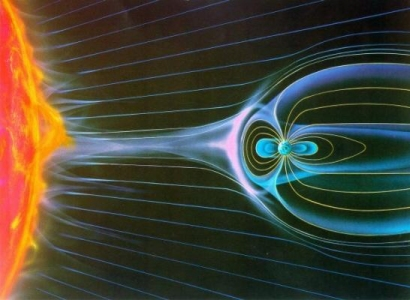
\includegraphics[scale=0.5]{images/NASA_BigPicture.jpg}
	\caption{The Sun, heliosphere, and magnetosphere (from NASA,
	\citeyear{SunHelMag}).}
    \label{fig:NASABP}
	\figSpace
\end{figure}
Figure \ref{fig:NASABP} shows a sketch of four space weather regions. The
starting point of all space weather is the Sun. The region that extends from the
solar surface to approximately 80-100 AU is called the heliosphere (the middle
region in Figure \ref{fig:NASABP} shows out to 1 AU)
\citep{Mewaldt1995}.
Inside the heliosphere are the planets, most of which have internally generated
magnetic fields that create a magnetic region known as a magnetosphere. Earth's
magnetosphere is shown on the right in Figure \ref{fig:NASABP}, its outer
boundary is defined at the location where the magnetic pressure of Earth's magnetic field
balances with the kinetic pressure of the plasma in the solar wind, and the
inner boundary is defined as the region where the exterior of Earth's
atmosphere interacts with the particles inside the magnetosphere, which is
called the ionosphere.

\subsection{Solar}
The 11-year variation in the measured solar magnetic flux and number of sunspots
defines the solar cycle \citep{Kallenrode}. All space weather originates at the
Sun, which consists mostly of fully ionized hydrogen and has a very strong magnetic field. The plasma near the
surface and the equator rotates faster than near the poles. The moving
plasma in the Sun causes its strong magnetic field \citep{Kulsrud}.

% SOLAR DYNAMO %
The solar dynamo, responsible for creating the Sun's magnetic field, is
due to the differential velocities of plasma near its surface
\citep{Kulsrud}. Differential rotation causes the magnetic field to twist and
stretch, which is defined as dynamo action. This
twisting and stretching causes increasing tensions in the solar magnetic field.
These associated poloidal and toroidal tensions cause
regions of increased surface magnetic field that appear on the solar surface as
sunspots.

% PARKER SPIRAL %
\begin{figure}
	\centering
	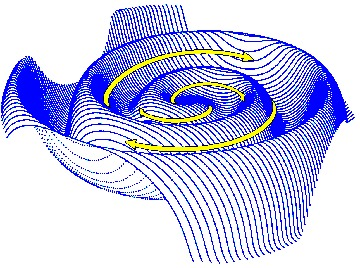
\includegraphics[scale=0.3]{images/parker.jpg}
	\caption{The Parker spiral (from NASA, \citeyear{ParkerSpiral}).}
	\label{fig:NASAParkerSpiral}
	\figSpace
\end{figure}
The twisting and stretching of the magnetic field causes the Sun to have a very
unique magnetic structure at times. Without a magnetic field, there would be a
constant flow of plasma radially outward. The presence of a magnetic field
causes changes in the location at which plasma escapes. There are different speeds of escaping plasma, and when
viewed in a cut plane of radial flow velocities in the heliosphere, a spiral
structure is expected as depicted in Figure \ref{fig:NASAParkerSpiral}.
\citet{Parker1958} first proposed the existence of this structure, now referred to 
as the Parker spiral.
% CIR %
\begin{figure}
	\centering
	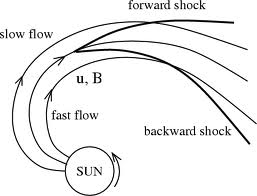
\includegraphics[scale=0.6]{images/CIR.jpeg}
	\caption{A co-rotating interaction region, (from \citeauthor{Volk2004},
	\citeyear{Volk2004}).}
	\label{fig:VolkCIR}
	\figSpace
\end{figure}
When different speeds of plasma flow outward from the Sun at different
latitudes, there are regions where fast moving plasma impacts slower moving
plasma (Figure \ref{fig:VolkCIR}) and results in a region of high density. These
regions of high density plasma are called co-rotating Interaction Regions (CIRs).

% sunspotS %
\begin{figure}
    \centering
    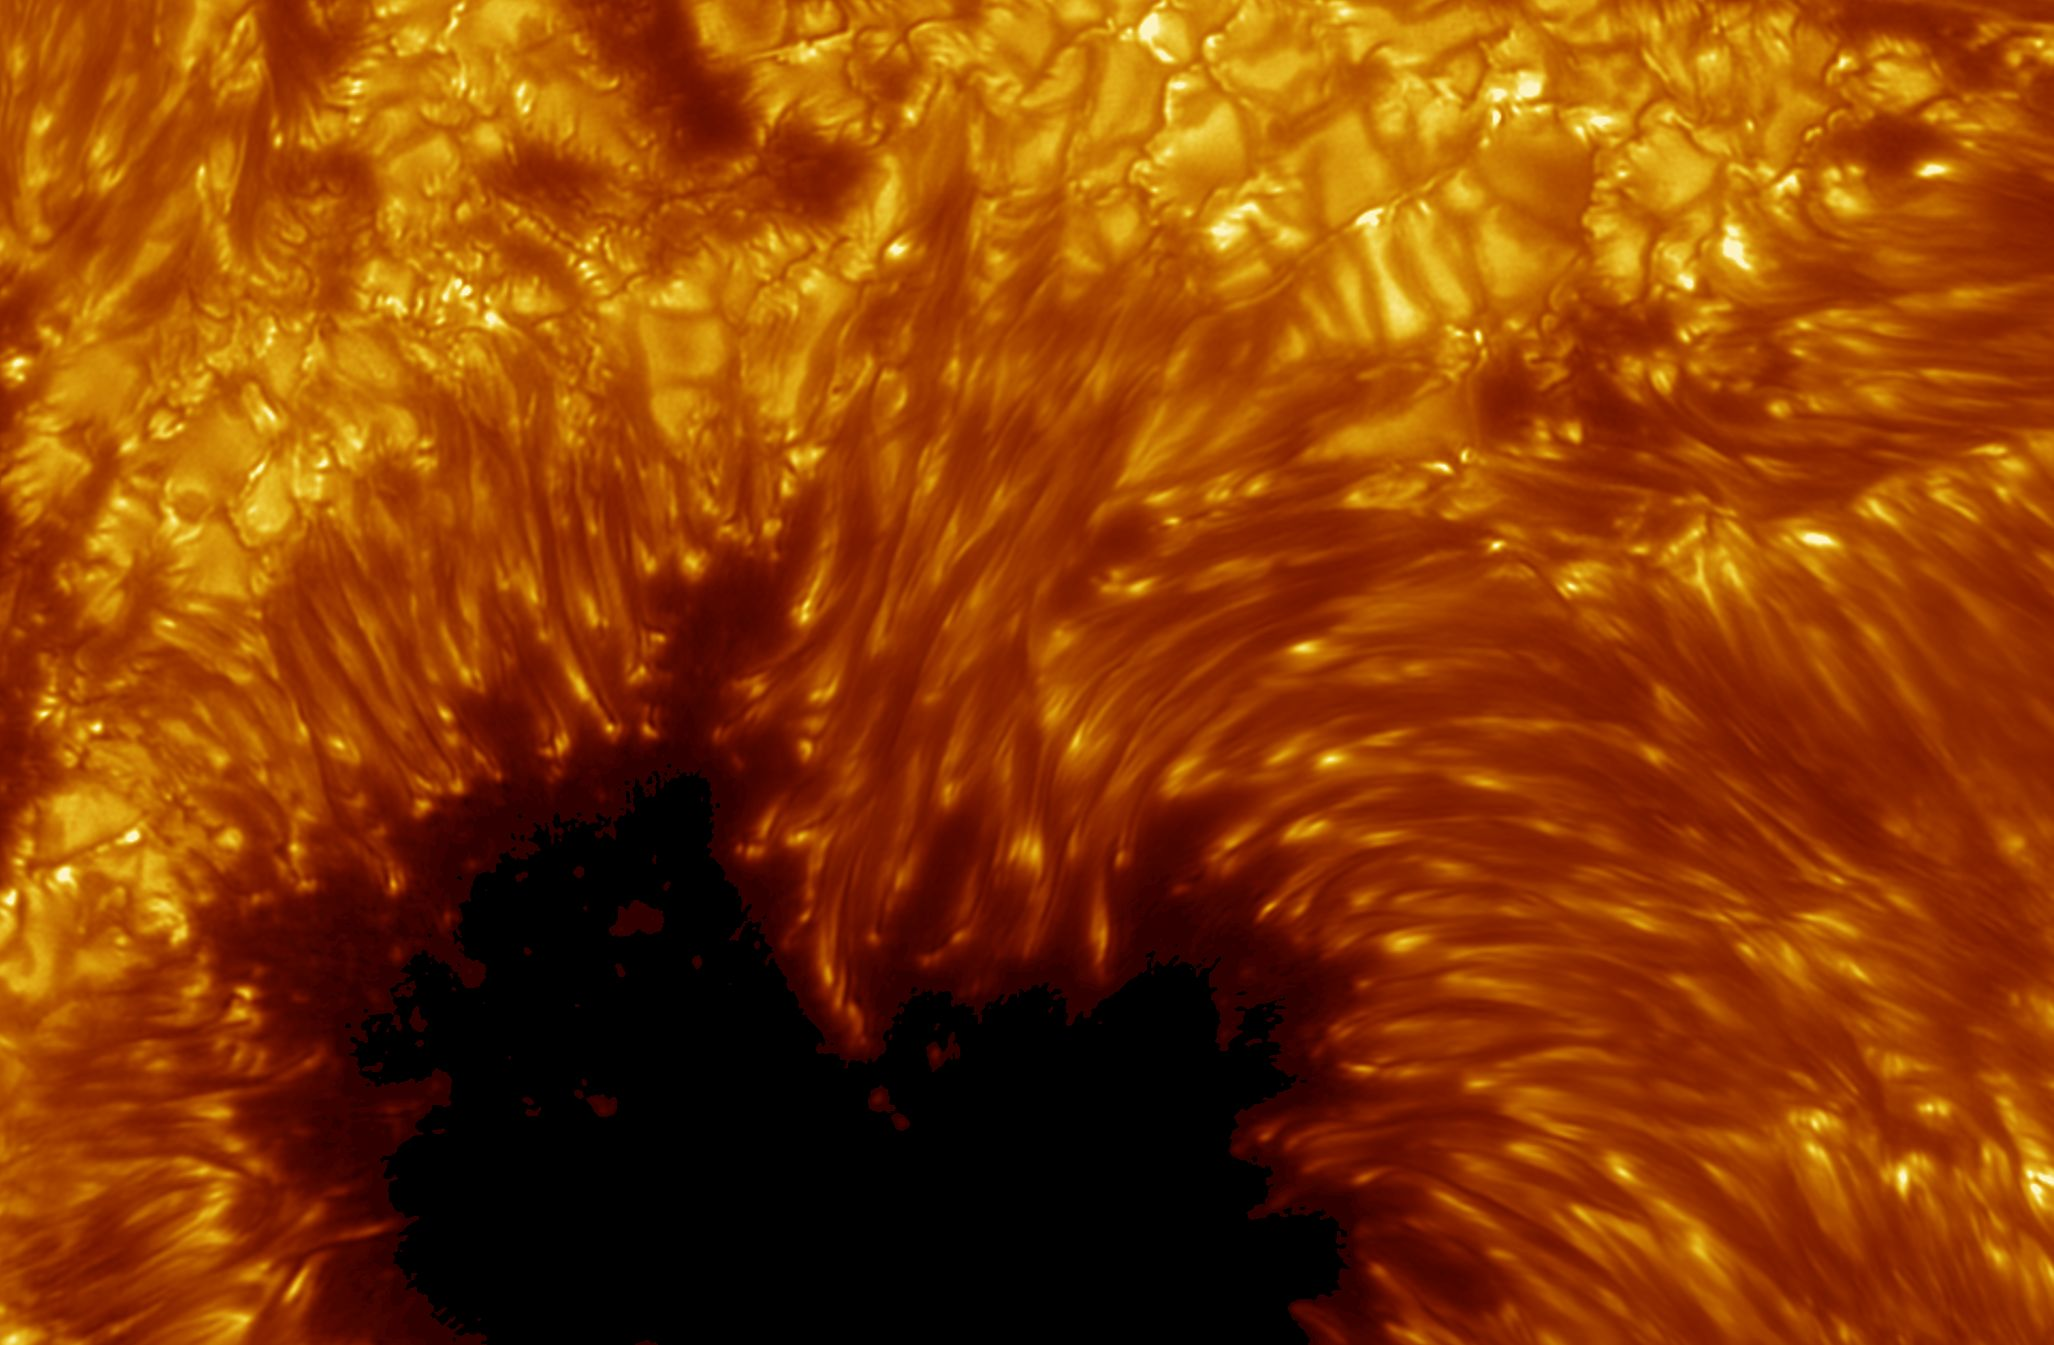
\includegraphics[scale=0.1]{images/NASA_Sunspot.jpg}\\
    \caption{A Sunspot (from NASA, \citeyear{Sunspot}).}
    \label{fig:NASAsunspot}
    \figSpace
\end{figure}
The most concern in space weather forecasting comes from events that are
associated with sunspots. Sunspots are regions of stronger magnetic field
strength on the solar surface. These regions have unique magnetic field
configurations that are believed to be related to the
cause of solar flares and Coronal Mass Ejections (CME) \citep{Kallenrode}.
Sunspots have a darker appearance as shown in Figure \ref{fig:NASAsunspot}. These regions have a
stronger magnetic field strength, giving them the darker appearance.

% SOLAR FLARES %
Solar flares are rapid bursts of energy released from the Sun. They are
typically observed as bright flashes in the visible $H_\alpha$ wavelengths.
Solar flares emit high-velocity ionized particles that can be very close to the speed of light and are used as warning signs that a CME may have occurred and could eventually be
measured by satellites near Earth (depending on their direction of
propagation).

% CME %
\begin{figure}
	\centering
	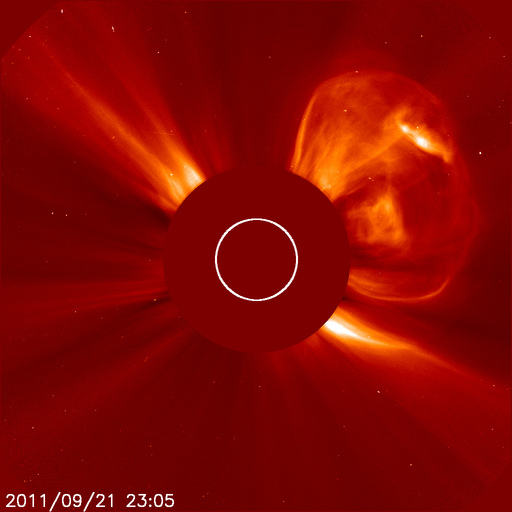
\includegraphics[scale=0.3]{images/NASA_CME.jpg}\\
	\caption{A coronal mass ejection (in the upper right corner of the image)
	taken from satellite imagery. The other two bright regions are called
	streamers (from NASA, \citeyear{CME}).}
	\label{fig:NASACME}
	\figSpace
\end{figure}
The name CME comes from satellite images showing large masses of plasma being
ejected away from the solar corona into the heliosphere, as shown in Figure
\ref{fig:NASACME}. The process that creates and drives CME	s is complex; this
process is the least understood space weather related phenomena. The plasma
associated with a CME has a shape similar to that of a light bulb and the
magnetic fields they carry are typically unorganized, complex, and difficult
to predict. Their cause is a subject of active research, but the generally
accepted explanation is that they are initiated as a result of reconnection
occurring near the sunspots \citep{Priest}.

\subsection{Heliosphere}
\begin{figure}
	\centering
	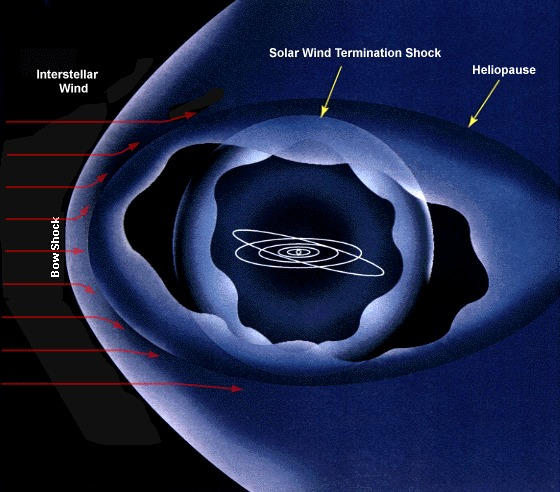
\includegraphics[scale=0.3]{images/NASA_Heliosphere.jpg}
	\caption{The heliosphere (from NASA, \citeyear{Heliosphere}).}
	\label{fig:NASAHelio}
	\figSpace
\end{figure}
The region exterior to the Sun and extending well beyond the orbit of Pluto is
called the heliosphere. Its exact shape is unknown, but an approximate tear
drop shape is depicted in Figure \ref{fig:NASAHelio}. The magnetic field it
contains decreases in strength with distance. Although the exact location of
the heliosphere boundary is unknown, it extends out well beyond the solar
system, and spacecraft have measured what is believed to be a heliopause at
approximately 120~AU \citep{Krimigis2009}. The spacecraft measurements included
a pause, sheath and shock region. These boundaries and region are explained in
detail in section \ref{MagnetosphereIntro}.

\subsection{Ionosphere/Thermosphere}
\begin{figure}
    \centering
    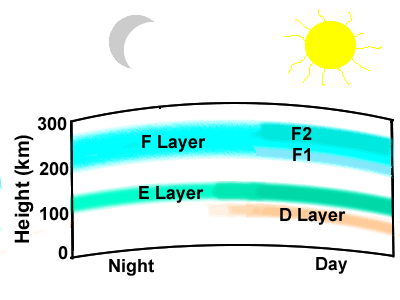
\includegraphics[scale=0.75]{images/ionosphere.png}
    \caption{The layers of Earth's ionosphere during the night time and the day
    time (from Naval Postgraduate School, \citeyear{Ionosphere}).}
    \label{fig:IonoThermo}
    \figSpace
\end{figure}
The ionosphere and thermosphere are contained within Earth's magnetosphere.
The ionosphere and thermosphere are overlapping layers that are considered
to be part of Earth's upper atmosphere, as shown in Figure \ref{fig:IonoThermo}.
The lower thermosphere boundary, which is located within the D and E regions of
the ionosphere, is defined by a rapid change in temperature, which is caused by
the absorption of ultraviolet (UV) and extreme UV (EUV) light. EUV radiation is
responsible for the creation of plasma on the sunlit side of the layer. The ionosphere has two different
profiles that are dependent on the time of day. The layers in each are labeled
as D, E, and F. The layers are defined by the density of the plasma. The F
region has the highest plasma density and is between 150-500 $km$. It is observed
more frequently in the summer time, and can separate when radiation from the
sun is highest. The E region is between 90-150 km
and the D region is below 90 km \citep{Kelley}. One importance of the ionosphere
is that high plasma densities can cause satellite drag.  Satellite drag
requires use of costly internal power resources, if available, to maintain altitude.

\subsection{Importance of Space Weather Research}
The Sun, heliosphere, magnetosphere, ionosphere, thermosphere, and all of their
phenomena are interconnected.
Understanding the thermosphere/ionosphere requires an understanding of the
magnetosphere. Understanding the magnetosphere requires an understanding of the
heliosphere. Understanding the heliosphere requires an understanding of the Sun.
As we learn more about one region, better analysis can be made in all
interconnected regions. The motivation for the pursuit of a better understanding
of space weather is due to the potential implications that adverse conditions
pose on terrestrial and space-based technology and operations.
These implications include increases in ground currents which can damage
electric power grids. HF and UHF communications can be disrupted, both of which
are vital to the air travel industry and the military. Earth-orbiting satellites
can be damaged from high energy particles. The global positioning system (GPS)
is linked to these satellites, and satellite damage could cause a loss of GPS
signals. Airplanes rely heavily on GPS. There are radiation exposure limits on astronauts
as well as humans on polar flights \citep{Pirjola2005}. The ability to
predict these adverse effects can help maintain the safety of humans in space
and ensure continual operation of space based technologies.

\subsubsection{Terrestrial Weather}
Meteorological observations in the United States have been recorded back as far
as the 17th century and were most often made along the east coast
\citep{Fiebrich2009}. Since then, significant improvements have been made. RADAR
technology used in World War 2 \citep{Page} was eventually used by the National
Weather Service (NWS). Automated Surface Observing Systems (ASOS) have been
placed throughout the country that record many meteorological conditions
\citep{Ahrens}. Today, meteorological forecasts are made and disseminated by
many sources including, but not limited to, radio stations, local television stations, the
private sector, and the government. These forecasts are made using the guidance
of forecast models. Meteorologists use the guidance of models to help make their
forecasts as accurate and precise as possible. The ability to understand all
meteorological models today would require a specific understanding of each
model. The abundance of forecasting models in the meteorology community would
make understanding each model a difficult task. With the increasing number of space weather
models, this gives motivation for improved methods for understanding forecasting
models.
\subsubsection{Space Weather}
The ability to measure space weather became possible with satellite technology.
The first satellites were launched in the late 1950s
and early 1960s \citep{Kallenrode}. In contrast to terrestrial weather, space
weather forecasts must use data that are sparse. For example, meteorology has data from ASOS to use as input data into models, which allow for the use
hundreds of input data points (ASOS, \citeyear{ASOSNum}). The sparsity of space
weather data forces forecasters to rely on numerical approximations of space
weather conditions that are not often corrected or modified by observations.
\subsubsection{Influence}
In meteorology, companies that fly airplanes or rescue teams, for example,
make decisions based on daily forecasts, and each decision has varying costs and
benefits \citep{Ahrens}. The same applies to space weather
forecasts. The companies that own and operate GPS satellites have
great interest in space weather forecasts.  For example, the airline
industry is interested in knowing whether to protect airplane
passengers by re-routing polar flights, which has varying costs and benefits
\citep{Lanzerotti2001}; \citep{Jones2005}. Finally, ground induced currents from
geomagnetic storms can effect electrical systems (GMDTF, \citeyear{GMDTF}).

\chapter{The Earth's Magnetosphere, Magnetohydrodynamics, and Magnetospheric
Models}
\section{Earth's Magnetosphere}
\label{MagnetosphereIntro}
\subsection{Discovery}
Research into the understanding of what would eventually be called the
magnetosphere started in the early 1600's when experiments were performed to
determine if garlic caused magnets to demagnetize. A similarity was found
between compass readings from a spherically shaped magnet and the direction of
mariners' compass readings. An inference was made that Earth was also a
magnet. Between the 1600's and mid-1900's there were many scientific advances in
the understanding of space weather. An important result from S.
Chapman and V. C. A. Ferraro in the early 1930's showed that solar streams were
not traveling along a direct path into Earth's upper atmosphere; they were being
deflected. Chapman and Ferraro estimated the deflection occurred at an upstream
boundary, which is known today as the Chapman-Ferraro boundary
\citep{Chapman1930}. In the 1950's, D. F. Martyn estimated the size of a
``geomagnetic hollow'' that Chapman and Ferraro predicted. This ``geomagnetic
hollow'' would eventually be named the magnetosphere by Thomas Gold in 1959.
Martyn estimated the distance to the boundary to be where the magnetic pressure
from magnetic field originating in Earth's core balanced the kinetic pressure
from a solar stream. In 1953, L. R. O. Storey researched whistlers caused from
lightning. Storey estimated that there must be plasma in the ``geomagnetic
hollow'' due to the way that Very Low Frequency (VLF) waves traveled between
Earth's hemispheres along field lines that passed through the magnetosphere.
When the U.S. and U.S.S.R. launched spacecraft to measure space weather parameters, they
found that plasma was trapped between Earth and the Chapman-Ferraro boundary,
which was not a part of the Chapman and Ferraro model of the magnetosphere
\citep{Kennel}.

\subsection{Shape}
\begin{figure}
    \centering
    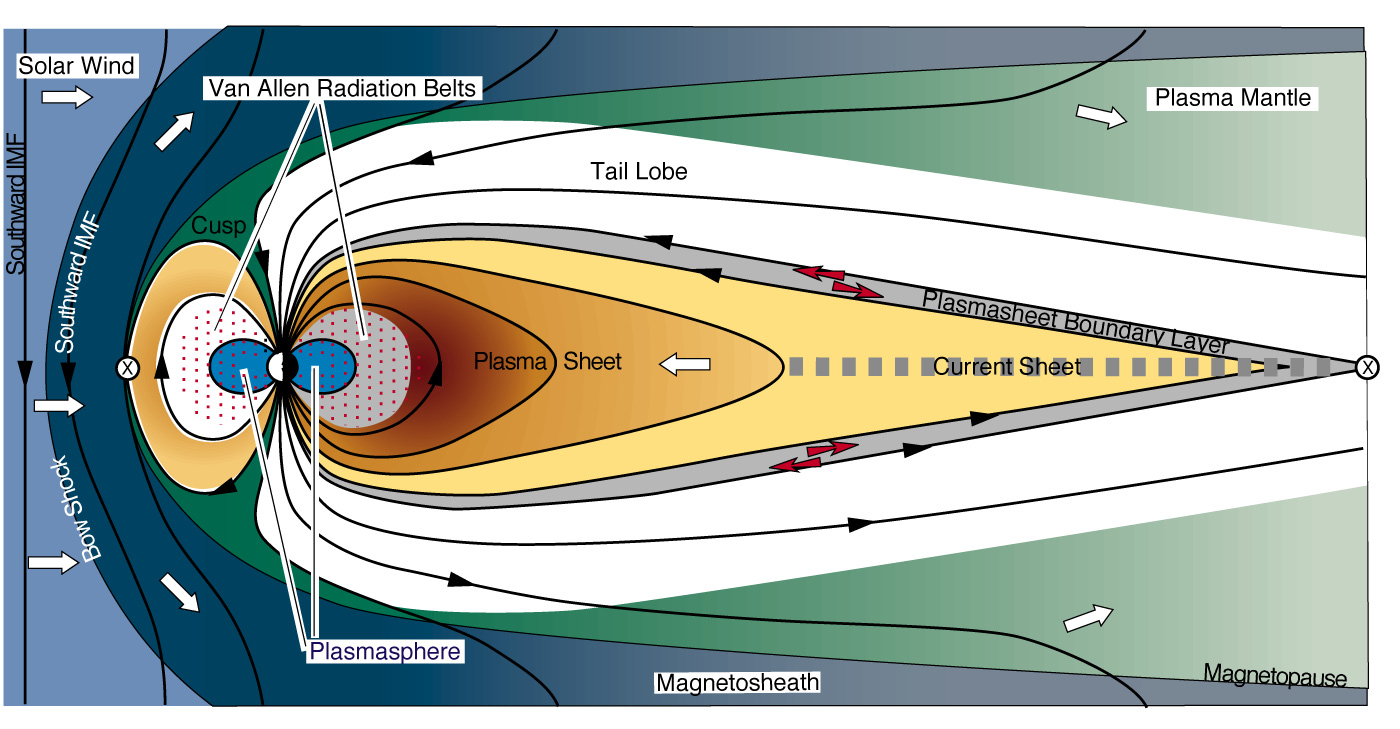
\includegraphics[scale=0.3]{images/Rice_Magnetosphere.jpg}
    \caption{The regions of Earth's magnetosphere (from Rice University,
    \citeyear{Magnetosphere}).}
    \label{fig:Rice_Magneto}
    \figSpace
\end{figure}
Based on the Chapman-Ferraro model, a calculation of the magnetopause
location could be made based on the balance between the kinetic pressure of the
solar wind and the magnetic pressure due to Earth's magnetic field. The
prediction of this model is a magnetopause at approximately 10 Earth radii
($R_E$), an overall teardrop shape, and a tail position between 50 and
100$R_E$. The processes that cause the bell shape in the magnetosphere are (1) viscosity
and reconnection and (2) change in solar wind density at the magnetopause.

\subsection{Reconnection}
Reconnection is a change in the topology of a magnetic field such that the
connectivity of field lines are changed in such a way that allows rapid conversion of
magnetic energy into kinetic energy. Reconnection is accepted to be the
source of the massive energy release associated with solar flares. Modern issues with reconnection involve questions about how such
a large amount of energy can be released in a very short amount of time.
Solar flares can release energy in the solar corona in approximately 100 seconds. Ideal
magnetohydrodynamics (MHD) can account for the time scale of energy release
but not for the amount of energy released. Non-ideal MHD accounts
for the release of a larger amount of energy but cannot match the short time
scales (Scholarpedia, \citeyear{Reconnection}). Two approaches were made to
describe how non-ideal MHD could have faster reconnection. One used a high
plasma resistivity, and the other used small dissipation scales. Sweet and Parker were the first to develop a MHD model
which had fast reconnection (by adding anomalous resistivity.) Another model was
devised by Petschek in 1964 in which the current sheet was thinner than that of
Sweet and Parker. This accounted for the small time scales and is accepted today
as the explanation for observations of fast reconnection \citep{Priest}.

\subsection{Reconnection in the Magnetosphere}
After the discovery that the solar wind was magnetized, \cite{Dungey1961}
proposed a new model of the magnetosphere that was significantly different from
the Chapman-Ferraro model.
In the Dungey model, field lines from the magnetosphere connect back into the
solar wind, as shown in Figure \ref{fig:Rice_Magneto}. The
Chapman-Ferraro model maps the fields lines between two hemispheres. Dungey's
model is considered open while the Chapman-Ferraro model is closed. Dungey's
model has two null points (shown as a white circles with an x in Figure
\ref{fig:Rice_Magneto}), which are regions where there is zero magnetic
field (and reconnection) due to the cancellation of opposing magnetic fields.
Dayside reconnection is primarily influenced by the orientation of the
interplanetary magnetic field (IMF). The magnetic field of Earth has a
northward orientation at the magnetopause. If the IMF is in the southward
direction, reconnection can occur. If the IMF direction is northward, minimal
or no reconnection occurs \citep{Priest}.

\subsubsection[The Reconnecting Magnetosphere]{The Reconnecting Magnetosphere}
\label{ReconnectingMagnetosphere}
The following section describes a long-supported view of the magnetosphere \citep{Kennel}.

\begin{figure}
	\centering
	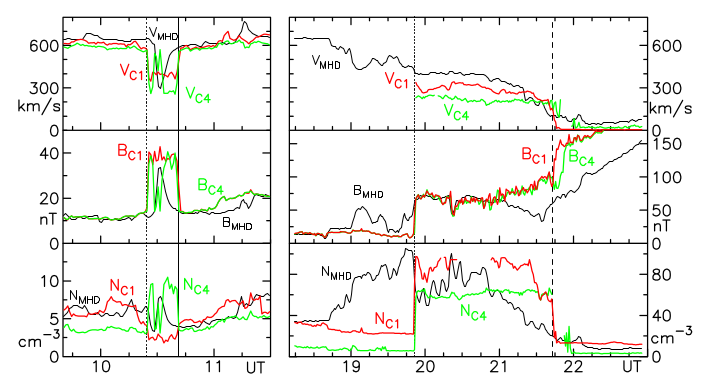
\includegraphics[scale=0.5]{images/MPandShock_VBN.png}
	\caption{Satellite measurements of velocity, magnetic field strength, and
	number density taken from Cluster 1 and Cluster 4 instruments as they
	cross through Earth's bow shock and magnetopause (from
	\citeauthor{Tatrallyay2012}, \citeyear{Tatrallyay2012}).}
    \label{fig:MPandShock_VBN}
	\figSpace
\end{figure}

\begin{figure}
	\centering
	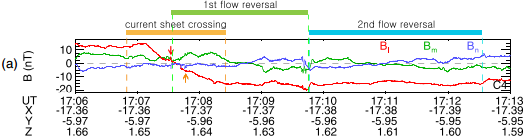
\includegraphics[scale=0.75]{images/Cur_sheet_B.png}
	\caption{Cluster 4 measurements of magnetic field strength as it crosses the
	current sheet in the magnetotail with time on the x axis; $l,m,n$
	represent current-sheet coordinates (from \citeauthor{Hwang2013},
	\citeyear{Hwang2013}).}
    \label{fig:Cur_sheet_B}
	\figSpace
\end{figure}

\begin{figure}
	\centering
	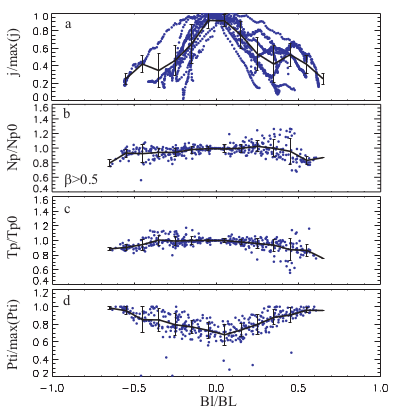
\includegraphics[scale=0.75]{images/Cur_sheet_N.png}
	\caption{Profiles of the (a) normalized current density, (b) normalized proton
	number density, (c) normalized proton temperature, (d) the sum of magnetic
	and ion pressures, versus normalized main magnetic field (from
\citeauthor{Runov2006}, \citeyear{Runov2006}).}
    \label{fig:Cur_sheet_N}
	\figSpace
\end{figure}
As shown in Figure \ref{fig:MPandShock_VBN} when passing through the bow shock
(in the Earthward direction), there is a velocity decrease, a $B$ increase at both the bow shock and magnetopause, density increase at the bow shock, and density decrease at the magnetopause.

During a magnetotail crossing, as shown in \citet{Runov2006} and
 \citet{Hwang2013}, there is a velocity increase as the distance from the
current sheet decreases. The magnetic field decreases and reverses direction as the current
sheet is crossed, as shown in Figure \ref{fig:Cur_sheet_B}. The number density
increases as the distance to the current sheet decreases, as shown in Figure
\ref{fig:Cur_sheet_N} \citep{Kennel}.

Based on many measurements similar to that described above for magnetopause and
magnetotail crossings, our general understanding of the reconnecting
magnetosphere is as follows and will be used for comparison to MHD model output
in the experiments performed:
\begin{itemize}
	\item $B_z$
	\begin{itemize}
	  \item When the $B_z^{IMF}$ is in the same direction of Earth's dipole, there
	  is a larger magnetic field strength and thus an increase in magnetic
	  pressure.
	  \item A negative $B_z^{IMF}$ and Earth's dipole oppose each
		other and decrease the magnetic pressure at the magnetopause. During these
		conditions field lines reconnect with the IMF and travel tailward.
	  \item When the magnetic pressure at the magnetopause decreases, the
	balance between the magnetic and kinetic pressures will change causing the
	magnetopause location to move Earthward.
	  \item Due to the stretching of the magnetic field tailward of Earth,
	oppositely directed magnetic field lines are moved closer causing the magnetic
	field in the current sheet region to approach zero.
	\end{itemize}
	
\item $\rho$
	\begin{itemize}
		\item As plasma travels Earthward from the Sun and encounters the magnetic
		field of Earth, it slows down. The plasma will eventually cross from
		supersonic to subsonic, creating a shock ahead of the magnetopause that is
		called the bow shock. Between the bow shock and magnetopause, plasma is
		compressed leading to higher densities.
		\item The stretching of magnetic field in the magnetotail causes oppositely
		directed magnetic field lines to become close enough to one another for
		reconnection to occur. This occurs in a plane called the current sheet and it
		separates the two opposing magnetic field directions. When reconnection occurs
		in the current sheet, a flow of new plasma replaces the plasma loss leading to
		an increase of densities. 
	\end{itemize}
	
	\item $U_x$
	\begin{itemize}
		\item The velocity of the plasma in the solar wind is supersonic. Inside the
		magnetosphere there is minimal solar wind velocity. As the
		solar wind is slows, there is a point at which it switches from supersonic to subsonic. This region is known
		as the bow shock.
		\item With the reconnection in the magnetotail occurring in the plasma sheet,
		there is a flow of plasma both towards and away from Earth on each side of
		the reconnection line. This movement is the reason that increases in
		velocities are observed as distance from the plasma sheet neutral line
		decreases.
	\end{itemize}
\end{itemize}

\subsection{Substorms}
The magnetosphere is constantly influenced by changes in the solar wind. The
direction of the IMF has the most influence. Energy from reconnection on the dayside magnetopause from a
southward IMF transfers to the magnetotail and causes a stretching of field
lines as they are dragged tailward by the solar wind. The stretching of the
field lines brings magnetic field lines of opposing direction close to one
another. Two opposing magnetic fields very close in proximity cause a sheet of
current to form. Reconnection causes a large amount of the stored
energy in the magnetotail to travel at high velocities towards Earth. The amount
of stored energy in each reconnection event is different, and so are the effects
measured at Earth. These events, as measured at Earth, are associated with substorms. On
the dayside, during times of southward IMF, the magnetopause position varies.
Many satellites have crossed the magnetopause boundary. In 1968, the OGO 5
satellite traveled towards Earth from the solar wind. The satellite recorded
approximately 10 magnetopause crossings. The first crossing was made when the
solar wind magnetic field was northward; shortly after this crossing, the
magnetic field turned southward and the satellite crossed the magnetopause once again, giving
the first measurement of the effects of southward IMF on the dayside
magnetopause. On the nightside, as the magnetopause shifts Earthward, the polar
cusps move towards the equator,	 and the thickness of the magnetotail increases
\citep{Kennel}.

\section{Magnetohydrodynamics}
\label{sec:mhd}
Magnetohydrodynamics describe the physics of magnetized fluid flow. Computational
models solve the MHD equations for a large number of points
in a specified domain.

\subsection{Single Species}
In 1872, Boltzmann derived equations that are used
today to describe the dynamics of a system that is not in thermodynamic
equilibrium. This is the starting point
for the derivation of the ideal MHD equations.
\subsubsection{Boltzman Equation}
The derivation of the single species MHD equations begins with the Boltzmann
equation for the probability distribution function
$f_s(\mathbf{x},\mathbf{v},t)$ of species s :
\begin{equation}
\frac{\partial f_s}{\partial t} + \mathbf{v} \cdot \nabla f_s + \mathbf{a}
\cdot \nabla_v f_s = \frac{\partial f_s}{\partial t}\bigg|_{coll}
\label{Boltzmann}
\end{equation}
Where $(\mathbf{x},\mathbf{v},t)$ represents position, velocity, and time,
respectively and $\mathbf{a}$ represents acceleration.
Multiplying equation \ref{Boltzmann} by a function of velocity
$\chi(\mathbf{v})$ and integrating over velocity gives:
\begin{equation}
\int \chi \frac{\partial f_s}{\partial t} d^3 \mathbf{v} + \int \chi \mathbf{v}
\cdot \nabla f_s d^3 \mathbf{v} + \int \chi \mathbf{a} \cdot \nabla_v f_s d^3
\mathbf{v} = \int \chi \frac{\partial f_s}{\partial t}\bigg|_{coll}  d^3
\mathbf{v}
\label{Boltzmann+1}
\end{equation}
This can be re-written as:
\begin{equation}
\frac{\partial}{\partial t}\int \chi f_s d^3 \mathbf{v} + \nabla \cdot \int
\mathbf{v} \chi f_s d^3 \mathbf{v} - \int f_s (\mathbf{a} \cdot
\nabla_v) \chi d^3 \mathbf{v} = \frac{\partial}{\partial t} \int \chi
f_s \bigg|_{coll} d^3 \mathbf{v}
\label{gentrans-1}
\end{equation}
where $\bigg|_{coll}$ refers to collisions between different species.

Using the definition of the average value $ < \chi >$ of a property $\chi$
of $n_s < \chi >_s = \int \chi f_s d^3 \mathbf{v}$, where $n_s$ is the number
density of species a, equation \ref{gentrans-1} becomes:
\begin{equation}
\frac{\partial}{\partial t}( n_s < \chi >_s) + \nabla \cdot (n_s < \chi
\mathbf{v} >_s) - n_s < ( \mathbf{a} \cdot \nabla_v) \chi >_s =
\frac{\partial}{\partial t} (n_s < \chi >_s)\bigg|_{coll}
\label{gentrans}
\end{equation}
which is the generalized transport equation \citep{Kominsky}.
\subsubsection{Conservation of Mass}
The law of the conservation of mass states that in a closed system the mass does
not change with time \citep{ConOfMass}. The equation for the conservation of
mass in MHD starts with equation \ref{gentrans}. For species with a mass $m_s$,
we can define:
\[ \chi = m_s \]
\[< \chi > = m_s\]
\[\mathbf{u_s} = < \mathbf{v_s} >\]
\[ \mathbf{v} = \mathbf{u_s} + \mathbf{c_s} \]
\[ < \mathbf{v_s} > = < \mathbf{u_s} + \mathbf{c_s} > \]
\[ < \mathbf{c_s} > = 0 \]
\[ < \chi\mathbf{v} >_s = m_s < \mathbf{v_s} > =  m_s \mathbf{u_s} \]
\[ \nabla_v \chi = 0 \]
Inserting these into equation \ref{gentrans} gives:
\begin{equation}
\frac{\partial}{\partial t} n_s m_s + \nabla \cdot (n_s m_s \mathbf{u_s}) = m_s
\int \frac{\partial f_s}{\partial t} \bigg|_{coll}
\label{ConOfMass-1}
\end{equation}
Defining the collision term $ S_s = \big( \frac{\partial \rho_s}{\partial t}
\big)_{coll}$, and with $\rho_s = n_s m_s$ gives:
\begin{equation}
\frac{\partial \rho_s}{\partial t} + \nabla \cdot (\rho_s \mathbf{u_s})
=  \bigg( \frac{\partial \rho_s}{\partial t} \bigg)_{coll} = S_s,
\label{ConOfMass}
\end{equation}
which is the equation for the conservation of mass \citep{Kominsky}.
\subsubsection{Conservation of Momentum}
The derivation of conservation of momentum is similar to that of mass.
Momentum cannot be created or destroyed and the amount of momentum in a specified
domain will remain constant in a closed system \citep{ConOfMomen}. Using
the property $m_s \mathbf{v}$ and defining $\chi = m_s \mathbf{v}$, equation
\ref{Boltzmann} can be written as:
\begin{equation}
\frac{\partial}{\partial t}(\rho_s < \mathbf{v} >_s) + \nabla \cdot (\rho_s <
\mathbf{v}\mathbf{v} >_s ) - n_s < (\mathbf{F_s} \cdot \nabla_v) \chi >_s = m_s
\int \mathbf{v} \bigg( \frac{\partial f_s}{\partial t} \bigg)_{coll}
\label{}
\end{equation}
Defining $\mathbf{v} = \mathbf{u}_s$ and $< \mathbf{c}_s >=0$ and solving for
$\nabla \cdot (\rho_s < \mathbf{vv} >_s)$ and $-n_s < (\mathbf{F_s} \cdot
\nabla_v) \chi >_s$ with the pressure tensor defined $P_s = \rho_s <
\mathbf{c_s c_s} >$, we arrive at the equation for the conservation of momentum \citep{Kominsky}:
\begin{equation}
\frac{\partial \rho_s \mathbf{u_s}}{\partial t} + \nabla \cdot
(\rho_s\mathbf{u_s u_s}) + \nabla \cdot (P_s) - n_s < \mathbf{F} > =
\mathbf{A_s}
\label{ConOfMomen}
\end{equation}
\subsubsection{Conservation of Energy}
The derivation of conservation of energy is similar to that of mass and
momentum. Energy cannot be created or destroyed and the amount of energy in a
specified domain will remain constant in a closed system \citep{ConOfEner}.
Starting with equation \ref{Boltzmann} and using the property $\frac{1}{2} m_s v^2$ and defining $\chi =
\frac{1}{2}m_sv^2=\frac{1}{2}m_s(\mathbf{v} \cdot \mathbf{v})$, then $\nabla_v
\chi = \frac{1}{2} m_s\nabla_v( \mathbf{v} \cdot \mathbf{v}) =
m_s(\mathbf{v}\cdot \nabla_v)\mathbf{v} = m_s\mathbf{v}$ gives:
\begin{equation}
\sum_s \frac{\partial}{\partial t} (\frac{1}{2}\rho_s < v^2 >_s) + \sum_s \nabla
\cdot (\frac{1}{2}\rho_s <v^2 \mathbf{v} >_s) - \sum_s n_s < \mathbf{F} \cdot
\mathbf{v} >_s = \frac{\partial}{\partial t}(\frac{1}{2} \rho_s < v^2
>_s)\bigg|_{coll}
\end{equation}
Solving for $\nabla \cdot (n_s < \chi \mathbf{v} >_s)$ , $- n_s < \mathbf{a}
\cdot \nabla_v \chi >_s$, and $< \mathbf{F} \cdot \mathbf{c_s} >$, this gives
an equation for conservation of energy:
\begin{equation}
\frac{\partial \epsilon_s}{\partial t} + \nabla \cdot (\epsilon_s \mathbf{u}_s)
+ \nabla \cdot (P_s \cdot \mathbf{u}_s) + \nabla \cdot \mathbf{q}_s -
n_sq_s\mathbf{u}_s \cdot \mathbf{E} - \rho_s\mathbf{u}_s \cdot \mathbf{g} = M_s
\label{ConOfEner}
\end{equation}
where $$\epsilon_s = \frac{p_s}{\gamma - 1} + \frac{1}{2} \rho_s u^2_s $$
$$P_s = \frac{1}{d} \sum_{ij} P_{aij}\delta_{ij} = \frac{1}{d}\sum_i P_{aii}$$
 $$\mathbf{q}_s = \frac{1}{2}\rho_s <c^2_s \mathbf{c}_s >$$
\subsection{Single Fluid}
The previous equations are applicable to each species in a plasma. To
allow for the treatment of the fluid as a whole, the individual species can be
summed. The following properties are defined by a sum over all species.
$$ \rho = \sum_s n_s m_s $$
$$ \rho \mathbf{u} = \sum_s n_s m_s \mathbf{u}_s $$
$$ \rho_q = \sum_s n_s q_s $$
$$ \mathbf{J} = \sum_s n_s q_s \mathbf{u}_s $$
\subsubsection{Conservation of Mass}
Using the above summations, equation \ref{ConOfMass} becomes:
\begin{equation}
\frac{\partial\rho}{\partial t} + \nabla \cdot (\rho \mathbf{u}) = 0
\label{FluidConOfMass}
\end{equation} 
\subsubsection{Conservation of Momentum}
Using the above summations, equation \ref{ConOfMomen} becomes:
$$ \sum_s \frac{\partial \rho_s \mathbf{u}_s}{\partial t} + \sum_s \nabla \cdot
(\rho_s \mathbf{u}_s \mathbf{u}_s) + \sum_s \nabla \cdot (P_s) - \sum_s
n_s(q_s(\mathbf{E} + \mathbf{u}_s \times \mathbf{B}) + m_s\mathbf{g}) = \sum_s
\mathbf{A}_s $$
Because the sum of the collision terms is zero, and total momentum is
conserved, the previous equation can be written as:
$$\frac{\partial \rho \mathbf{u}}{\partial t} + \nabla \cdot \sum_s \rho_s
\mathbf{u}_s \mathbf{u}_s + \nabla \cdot \sum_s P_s - \rho_q\mathbf{E} -
\mathbf{J} \times \mathbf{B} - \rho \mathbf{g} = 0 $$
Solving for the summations results in an equation for the conservation of
momentum for a single fluid:
\begin{equation}
\frac{\partial \rho \mathbf{u}}{\partial t} + \nabla \cdot (\rho
\mathbf{u u}) + \nabla \cdot P - \rho_q\mathbf{E} - \mathbf{J}
\times \mathbf{B} - \rho \mathbf{g} = 0
\label{FluidConOfMomen}
\end{equation}
\subsubsection{Conservation of Energy}
Using the above summations, equation \ref{ConOfEner} becomes:
$$ \sum_s \frac{\partial \epsilon_s}{\partial t} + \sum_s \nabla \cdot
(\epsilon_s \mathbf{u}_s + P_s \cdot \mathbf{u}_s + \mathbf{q}_s) - \sum_s n_s
q_s \mathbf{u}_s \cdot \mathbf{E} - \sum_s \rho_s \mathbf{u}_s \cdot \mathbf{g}
= 0 $$
Upon solving for $ \sum \rho_s u_s^2 $, $\sum_s \epsilon_s $, and $\sum_s p_s
\mathbf{u_s} $, where the total scalar pressure is
$$p = \frac{1}{d} \sum_i P_{ii} = \frac{\gamma - 1}{2} \sum_s \rho_s < ( c_s
+ w_s)^2 > = \sum_s p_s + \frac{\gamma -1}{2} \sum_s \rho_s w_s^2,$$
and the total heat flux is
$$ \mathbf{q} = \frac{1}{2} \sum_s \rho_s < (c_s + w_s)^2(\mathbf{c}_s +
\mathbf{w}_s) > ,$$
this gives conservation of energy:
\begin{equation}
\frac{\partial \epsilon}{\partial t} + \nabla \cdot (\epsilon \mathbf{u} + P
\cdot \mathbf{u} + \mathbf{q}) - \mathbf{J} \cdot \mathbf{E} - \rho\mathbf{u}
\cdot \mathbf{g} = 0.
\label{FluidConOfEner}
\end{equation}
\subsubsection{Maxwell's Equations}
Maxwell's equations relate $\mathbf{E}$, $\mathbf{J}$, and $\mathbf{B}$ from the
previous plasma equations:
\\Gauss's law:$$ \nabla \cdot \mathbf{E} = \frac{\rho_q}{\epsilon_0}$$
Gauss's law for magnetism: $$ \nabla \cdot \mathbf{B} = 0 $$
Faraday's law:$$ \nabla \times \mathbf{E} = - \frac{\partial
\mathbf{B}}{\partial t} $$ 
Ampere's law:$$ \nabla \times \mathbf{B} = \mu_0(\mathbf{J} + \epsilon_0
\frac{\partial \mathbf{E}}{\partial t}) ,$$
where $\mu_0$ is the permeability, $\epsilon_0$ is the permittivity,
$\mathbf{E}$ is the electric field, $\mathbf{B}$ is the magnetic field,
$\mathbf{J}$ is the current, and $\rho_q$ is the charge density.
\subsubsection{Conservation of Current Density}
Using Maxwell's equations, the single species momentum
equation multiplied by $\frac{q_s}{m_s}$ and summed over species
gives:
$$ \frac{\partial}{\partial t} \sum_s n_s q_s \mathbf{u}_s + \nabla \cdot
(\sum_s n_s q_s \mathbf{u}_s \mathbf{u}_s) + \nabla \cdot (\sum_s
\frac{q_s}{m_s} P_s) - \sum_s n_s \frac{q_s}{m_s} < \mathbf{F} > = \sum_s
\frac{q_s}{m_s} \mathbf{A}_s$$ Noting that:
$$ \mathbf{J} = \sum_s n_s q_s \mathbf{u}_s $$
gives conservation of current density:
\begin{equation}
\frac{\partial \mathbf{J}}{\partial t} + \nabla \cdot (\mathbf{J u} + \mathbf{u J} 
- \rho_q \mathbf{uu} + \mathbf{P}_q) - \sum_s n_s \frac{q_s}{m_s} < \mathbf{F}
> = \sum_s \frac{q_s}{m_s} \mathbf{A}_s
\end{equation}

\subsection{Ideal}
To simplify the single fluid MHD equations, the following
assumptions are made:
\begin{itemize}
\item The time derivative of E is small.
\item Isotropic Pressure: \\
If the pressure tensor $P$ is replaced with $p\mathbf{I}$, then $\nabla \cdot P
= \nabla p$.
\item Charge neutrality: $\rho_q = 0$.
\item Neglect small terms: \\
Terms involving $P_q$ can be neglected if $p_e$ is small.
\item Single ion flow with collision term approximation: \\
Used to simplify the magnetic field differential equation.
\item Perfect conductivity: \\
$\sigma$ is infinite so that $\mathbf{E} + \mathbf{u} \times \mathbf{B} =
\frac{\mathbf{J}}{\sigma} \simeq 0$, giving $\mathbf{E} = - \mathbf{u} \times
\mathbf{B}$
\end{itemize}

Using these assumptions along with Maxwell's equations, the conservation equations become \citep{Kominsky}:
\begin{itemize}
  \item Conservation of Mass
  $$ \frac{\partial \rho}{\partial t} + \nabla \cdot (\rho \mathbf{u}) = 0$$
  \item Conservation of Momentum
  $$ \frac{\partial \rho \mathbf{u}}{\partial t} + \nabla \cdot \left[\rho
  \mathbf{uu} + (p + \frac{B^2}{2\mu_0})\mathbf{I} - \frac{1}{\mu_0}
  \mathbf{BB}\right]- \rho \mathbf{g} = 0$$
  \item Conservation of Energy
  $$ \frac{\partial \epsilon}{\partial t} + \nabla \cdot \left[( \epsilon + p +
  \frac{B^2}{2\mu_0})\mathbf{u} + \mathbf{q} - \frac{1}{\mu_0}(\mathbf{u} \cdot
  \mathbf{B}) \mathbf{B}\right] - \rho \mathbf{u} \cdot \mathbf{g} = 0 $$
  \item Conservation of Magnetic Flux
  $$ \frac{\partial \mathbf{B}}{\partial t} + \nabla \cdot (\mathbf{uB} - \mathbf{Bu}) = 0 $$
\end{itemize}

\section{Magnetospheric Models}
To most accurately model the magnetosphere, the collisionless Boltzmann equations for individual species
along with Maxwell's equations should be used. The use of these equations in a
computational model is costly because the computational complexity of the
algorithms for their solutions are high \citep{Raeder2003}. A more efficient solution is
to use the ideal MHD equations. In the magnetospheric community, there are three
often-used models that implement ideal MHD. The way that each magnetospheric
model approaches these equations gives them their uniqueness.

\subsection{Grid and Geometry}
Each model uses a choice of a numerical grid and numerical method to solve the MHD equations. For the
magnetosphere, Earth's magnetopause can expand to tens of Earth radii
towards the Sun, so the simulation domain for the grid must be at least this large.
The tailward boundary can be $\ge$ 200 $R_E$, and the transverse regions are
typically $\ge$ 50 $R_E$. The choice for the numerical grid resolution and size
depends on the computational resources; the grid choice is also influenced by
the numerical method. Grids used in MHD models include:
\begin{itemize}
  \item Uniform Cartesian \\
  \begin{figure}
  	\begin{centering}
  	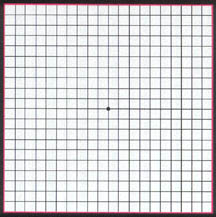
\includegraphics[]{images/UniformCartesian.jpg}
  	\caption{Uniform Cartesian Grid (from StackOverflow, \citeyear{UnifCart}).}
  	\label{fig:UniformCartesian}
  	\end{centering}
  	\figSpace
  \end{figure}
  Uniform grids as shown in Figure \ref{fig:UniformCartesian} have equal spacing
  in all dimensions.
  The amount of programming required and the computational resources used are low, and parallelization is the most straightforward to implement. The most significant limitation of the uniform cartesian
  grids is that the same resolution must be used everywhere in the domain. The optimal
  resolution is not necessarily the same for all regions of the domain.
  
  \item Stretched Cartesian \\
  \begin{figure}
  	\begin{centering}
  	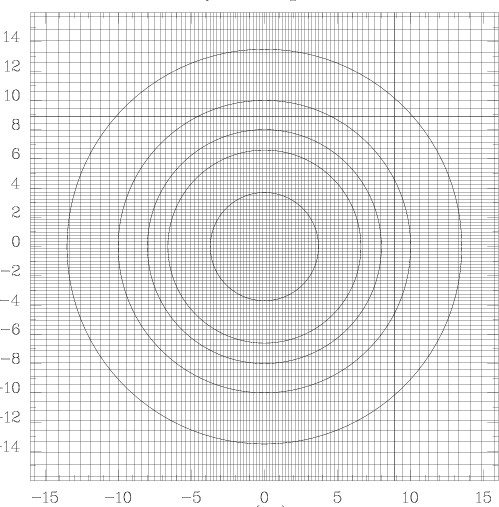
\includegraphics[scale=0.45]{images/StretchedCartesian.jpg}
  	\caption{Stretched Cartesian Grid (from Univeristy of New Hampshire,
  	\citeyear{StretchCart}).}
  	\label{fig:StretchedCartesian}
  	\end{centering}
  	\figSpace
  \end{figure}
  Stretch Cartesian grids, as shown in Figure \ref{fig:StretchedCartesian}, can
  be ``stretched'' in each dimension while still maintaining the ease of
  programming comparable to a uniform cartesian grid. The stretching can allow
  for higher resolution in regions around Earth, magnetopause, and bow
  shock regions, and other regions where needed, and lower resolution in areas
  that do not need it such as the distant magnetotail. Specifically for the
  magnetosphere, this grid type is very well adapted.
  
  \item Structured Adaptive Mesh Refinement (SAMR) \\
  \begin{figure}
  	\begin{centering}
  	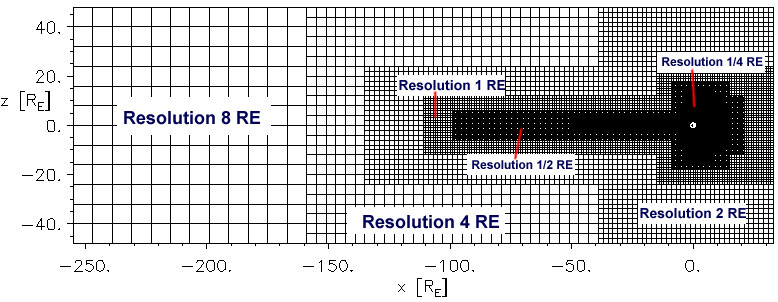
\includegraphics[scale=0.45]{images/SAMR.JPG}
  	\caption{Structured Adaptive Mesh Refinement Grid (from NASA,
  	\citeyear{SAMR}).}
  	\label{fig:SAMR}
  	\end{centering}
  	\figSpace
  \end{figure}
  SAMR grids, similar to that shown in Figure \ref{fig:SAMR}, have higher
  grid resolutions in regions that need it. These higher resolutions are
  added and removed as time progresses as needed. Different
  refinements are possible, which requires a larger coding and computational
  resource cost, yet SAMR can provide the
  most accurate solutions \citep{Raeder2003}.
  
  \item Unstructured Grid \\
  \begin{figure}
  	\begin{centering}
  	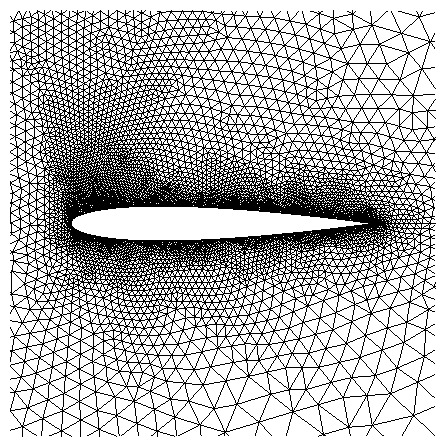
\includegraphics[scale=0.45]{images/Unstructured.jpg}
  	\caption{Unstructured Grid (from Delft University of Technology,
  	\citeyear{Unstruc}).}
  	\label{fig:Unstructured}
  	\end{centering}
  	\figSpace
  \end{figure}
  In an unstructured grid, as shown in Figure \ref{fig:Unstructured}, the shape
  of each cell is typically different than its neighbors. These grids are
  typically used in finite element and finite volume methods. They are very
  difficult to program, computationally expensive, and are difficult to
  parallelize. Their major benefit is the ability to form well to the object
  they model.
\end{itemize}

\subsection{Boundary Conditions}
On the sunward side of the grid boundary, the boundary conditions can be fixed
or time dependent. As solar wind data is measured at only a few points
near the boundary, it is difficult to determine the extended structure of the
solar wind boundary conditions. On all other boundaries, free flow conditions apply
with the exception that the $\nabla \cdot \mathbf{B} = 0$ condition is used to derive the
normal of the magnetic field (and should be consistent with the numerical
scheme) \citep{Raeder2003}.

\subsection{Initial Conditions}
\label{InitialConditions}
On the sunward side of Earth, there is a region where its magnetic field
reaches near zero. The initial conditions for $B$ are created by placing a
mirror dipole sunward of Earth such that a plane with zero magnetic field exists
close to Earth on the sunward side.
The initial solar wind and magnetic field then replaces the mirror dipole
sunward of the near zero B region.
The plasma initial conditions are typically set at a temperature of
$5000$ [$^\circ$K] and a density of $0.1$ [$cm^{-3}$]. With these initial
conditions, it can take up to ond hour for the magnetosphere to start forming. Because
the magnetosphere has a memory of previous conditions that can last
many hours, it is important to allow at least a few hours of preconditioning
time before using input data for a specific event \citep{Raeder2003}. To date,
no evaluation of the influence of preconditioning on model results has been
published.

\subsection{Spatial Discretization}
There are four different approaches used for spatial discretization in MHD
models of the magnetosphere: finite differences, finite volumes, finite
elements, and spectral.

Finite difference methods are most used in magnetospheric models, and some of
the concepts from finite differencing schemes are found in the other methods.
Conservative finite difference schemes have the best fit for global MHD
simulations \citep{Raeder2003}.

\subsection{Numerical Implementation}
There are simple differencing schemes that can have 2nd order accuracy.
Schemes such as predictor-corrector and leap-frog can be accurate,
but they lack stability, which is required in a majority of the computational
domain. The Courant-Friedricks-Levy (CFL) criteria limits the timestep for
stability. The Alfv\'en speed can be extremely large. A ``Boris Correction" or
some variant is used to limit the Alfv\'en speed allowing for larger time steps
without increasing errors in the solution \citep{Raeder2003}.

\subsection{The Open Global Geospace Circulation Model}
The Open Global Geospace Circulation Model (OpenGGCM) solves the ideal MHD
equations for the magnetosphere using a conservative finite
difference method for the gas dynamic part of the normalized ideal MHD equations.
The equations solved are: $$ \frac{\partial \rho}{\partial t} = -\nabla \cdot
(\rho \mathbf{v}) $$ $$ \frac{\partial \rho \mathbf{v}}{\partial t} = -\nabla \cdot (\rho \mathbf{vv} +
pl)+ \mathbf{j} \times \mathbf{B}$$ $$ \frac{\partial e}{\partial t} = -\nabla
\cdot (\{e+p\}\mathbf{v}) + \mathbf{j} \cdot \mathbf{E} $$ $$ \frac{\partial
\mathbf{B}}{\partial t} = - \nabla \times \mathbf{E} $$ $$ \nabla \cdot
\mathbf{B} = 0 $$ $$ \mathbf{E} = -\mathbf{v}\times\mathbf{B} = \eta \mathbf{j}
$$ $$ \mathbf{j} = \nabla \times \mathbf{B} $$ $$ e = \frac{1}{2} \rho v^2 +
\frac{p}{\gamma -1} $$ The OpenGGCM treats the $\mathbf{j} \times \mathbf{B}$
and $\mathbf{E} \cdot \mathbf{j}$ terms as source terms due to low plasma beta (the ratio of plasma pressure to the magnetic pressure)
and large gradients in the magnetic field that do not allow for a full
conservative formalism. The magnetic field is initialized with the superposition of 
Earth's dipole such that at approximately 16$R_E$, $B_z$ is zero. After
this, the magnetic field from 16$R_E$ sunward is replaced by the initial solar wind
magnetic field. This ensures the $\nabla \cdot \mathbf{B} = 0$ condition for
ideal MHD is met (CCMC, \citeyear{CCMCOpenGGCM}).

\subsection{The Block Adaptive-Tree Source Roe-type Upwind Scheme Model}
The Block Adaptive-Tree Source Roe-type Upwind Scheme (BATS-R-US) model uses a
finite volume discretization and solves the conservative MHD equations:
$$ \frac{\partial \rho}{\partial t} + \mathbf{u} \cdot \nabla p + \rho\nabla
\cdot \mathbf{u} = 0 $$ $$ \rho \frac{\partial \mathbf{u}}{\partial t} + \rho
\mathbf{u} \cdot \nabla \mathbf{u} +  \nabla p - \mathbf{j} \times \mathbf{B} =
0 $$ $$ \frac{\partial \mathbf{B}}{\partial t} + \nabla \times \mathbf{E} = 0 $$
$$ \frac{\partial p}{\partial t} + \mathbf{u} \cdot \nabla p + \gamma p \nabla
\cdot \mathbf{u} = 0 $$ $$ \mathbf{j} = \frac{1}{\mu_0} \nabla \times \mathbf{B}
$$ $$ \mathbf{E} = -\mathbf{u} \times \mathbf{B} $$ The $\nabla \cdot
\mathbf{B}$ constraint can be implemented using four different divergence
control schemes. The eight wave, diffusive/parabolic, projection, and a conservative
form of the constrained transport scheme extended to adaptive grids.
The grid is set using an adaptive mesh refinement technique. This
technique adapts specific sections of the computational domain so that areas
where higher resolution or lower resolution are most appropriate can be used.
If a higher resolution is needed, then a cell is divided into eight children.
When lower resolution is needed, a block of eight is
grouped into one cell. Initial conditions at boundaries of the computational
domain are set to solar wind conditions and the mirror dipole method described previously is used.


\chapter{Validation}
\section{Overview}
Validation and Verification analyses help model users and developers gain a
greater confidence and understanding of the accuracy of model output and its numerical
implementation, respectively. Validation analyses are most often used to show
the user community how the model output compares with measured data.
Verification analyses are used to ensure that the numerical implementation of
the mathematics are correct.

Model validation encompasses many ways of looking at model output
\citep{Sargent2004}. There are many different methods of validation, and the
appropriate method for a specific model depends on its intended use. Sargent
\citet{Sargent2004} describes fifteen different methods of validation:
\begin{itemize}
  \item \textbf{Animation}: The output of the model is plotted graphically
  over a time range.
  \item \textbf{Comparison to other models}: The results from previously
  validated models are compared to that of a new model.
  \item \textbf{Degenerative tests}: The degeneracy in the behavior of the model
  is tested with a specific selection of input and internal parameters that are
  expected to result in degenerate model output.
  \item \textbf{Event validity}: Important events predicted by a model are
  compared to the important events of the real system.
  \item \textbf{Extreme condition test}: The output of the model should be
  plausible even when unlikely or rare conditions are input into the system
  initially.
  \item \textbf{Face validity}: Discussing the models output with scientists who
  are experienced and knowledgeable about the modeled system.
  \item \textbf{Historical Data Validation}: If historical data exists, it
  is used as input into a model and the output is compared to the real
  system.
  \item \textbf{Historical methods}
  \item \textbf{Internal validity}: Several runs with the same input are made to
  determine the amount of variability in the model. The larger the variability,
  the larger the questionability of the model. 
  \item \textbf{Multistage validation}: Using multiple validations at once.
  \item \textbf{Operational graphics}: Various model forecast performance
  measures are graphically displayed as the model progresses through time.
  \item \textbf{Parameter variability - sensitivity analysis}: Changing the
  input and internal values of a model to determine the effect of the model's
  output/behavior.
  \item \textbf{Predictive validation}: Models are used to predict the system's
  behavior, and comparisons are made to the system's actual behavior to
  determine if they are similar.
  \item \textbf{Traces}: The internal behavior of the model is followed to
  determine if the logic in the model is correct and the needed accuracy is
  obtained.
  \item \textbf{Turing tests}: Scientists knowledgeable about the system are
  asked to determine if they can distinguish a model from the measurements from the
  modeled system.
\end{itemize}

\citet{Sargent2004} defines two basic approaches to verification of
computational models as static and dynamic testing.
\begin{itemize}
 \item \textbf{Static Testing}:  In static testing, the model is
 analyzed for correctness by using techniques such as structured walk-throughs,
 correctness proofs, and examining the structure properties of the program.
 \item \textbf{Dynamic Testing}: In dynamic testing, the model is
 tested with differing conditions where the data received is used to determine
 if the program has correct implementations. Four dynamic tests described by
 Sargent are traces, investigations of input-output relations using different
 validation techniques, internal consistency checks, and reprogramming critical
 components to determine if the same results are obtained.
\end{itemize}

The following two subsections contain examples of the types of validation currently
used in both terrestrial weather and space weather. Research on terrestrial
weather prediction models have involved primarily \textit{parameter variability} studies
that test the physics of the model using artificial input parameters. Research
on space weather prediction models have involved primarily \textit{predictive
validation} using measured solar wind input data.
\section{Terrestrial Weather Validation}
Terrestrial weather models have been in operation by the NWS longer than space
weather models have with the Space Weather Prediction Center (SWPC). Terrestrial
weather methods of validation have been improved over that time and their validation methods
should be considered for space weather modeling.

A majority of terrestrial weather models used for prediction use the comparison
to other models validation technique described in \citep{Sargent2004}. This is
similar to what is currently done with space weather models used in prediction. The
following terrestrial weather models, both for weather and climate prediction,
show \textit{predictive} and \textit{parameter variability - sensitivity
analysis} validation techniques, respectively. The following three examples are representative of
modern terrestrial weather validation.

\citet{Boznar2012} validates a short-term fine-resolution Weather Research
and Forecasting (WRF) model by comparing its output to observations made in
Slovenia. The complex terrain in Slovenia can cause problems with wind profiles
in the models, and the motivation for this analysis was to determine how
extremes in height were handled by the model. They found that the model
performed better with stations that were on top of hills and worse with
stations that were in basins and valleys. This is an example of
\textit{predictive validation}.

\citet{Molteni1996} performed a sensitivity analysis on the European
Center for Medium-range Weather Forecasts (ECMWF) model in which a perturbation was input
into the model to determine how it affected the output as a part of
a larger validation effort. This is an example of a \textit{parameter
variability - sensitivity analysis}.

\citet{Andrejczuk2006} performed simulations of cloud-clear air
interfacial mixing. In this study they use initial velocity fields made from high, moderate,
and low intensity levels of turbulent kinetic energy input into the models. This
is also an example of \textit{parameter variability} as they use a variety of input
conditions and then evaluate the model output.

\citet{Katzav2011} argued that severe testing of climate model
predictions (CMPs) should have a larger role in the assessment of CMPs. Severe testing is a
\textit{parameter variability} validation in which input variables are set to
extreme values.
\citet{Katzav2011} suggested that the current view on model assessment, that CMP
quality should depend on simulation accuracy, is insufficient reasoning and explains
that severe testing addresses concerns about relying on successes that are
based on results obtained from data accommodation. Secondly, severe testing
helps test the maturity of the science underlying CMPs. Lastly, Katzav suggests
that even though some severe testing may already occur, it is not nearly enough,
and increased severity testing will help science progress. Severe testing is
the term used by Katzav and is similar to \textit{parameter variability}.
\textit{parameter variability} and severe (extreme condition) testing will be used in this
dissertation.

\section{Space Weather Validation}
\label{SpaceWeatherVV}
With a lack of measurements in the Sun-to-Earth domain, MHD modeling has been a
key to predictive analysis in space weather, especially in regions where dense
or long-term measurement do not exist. In recent years, there has been an
increasing amount of attention to validation in the space weather modeling community
as interest in transitioning models into operations increases. The number
of space weather researchers that use \textit{parameter variability} validation is limited. The
following examples do not use \textit{parameter variability} validation, but
rather show the large use of the \textit{comparison to other models} validation technique.

\citet{Taktakishvili2009} used a combination of the halo CME analytical “cone
model” \citep{Xie2004} and the Enlil solar wind model \citep{Odstrcil2003}  to predict the CME arrival time at Earth using historical solar wind
data. This is \textit{historical data} validation. Because they also
compared their results with two other models, they also employed the
\textit{comparison to other model} validation technique.

\citet{Pulkkinen2011} compared ground magnetometer
predictions made by fourteen different models to the measurements made from
twelve different geomagnetic observatories and used four different metrics to quantify the model
performance for four different storm events. The three validation tests they
used can be classified as \textit{comparison to other models},
\textit{predictive validation}, and \textit{historical data} validation.

\citet{MacNeice2009a} documented a set of procedures to test the prediction
capability of the Wang-Sheeley-Arge (WSA) model \citep{Arge2003}.
\citet{MacNeice2009b} discussed model results using data taken from the
solar wind at Earth up to four days in advance of geomagnetic storms. Both
papers used a \textit{predictive validation} technique.

\citet{Garcia2007} performed a statistical comparison between the
Lyon-Fedder-Mobarry magnetosphere MHD-based model \citep{Lyon2004} and
empirical models of the magnetopause location to determine which better
predicted the actual position of the magnetopause. This is an example of the
\textit{comparison to other models} validation technique.

\citet{Mozer2003} used the forecasts of 96 solar wind shocks at the
L1 point made by the Hakamada-Akasofu-Fry (HAF) model \citep{Hakamada1982} and
compared it to real time data from the solar wind electron proton alpha monitor
(SWEPAM) and MAG (magnetometer) instruments on the Advanced Composition
Explorer (ACE) spacecraft \citep{Stone1998}. This is an example of the
\textit{historical data validation} as well as \textit{predictive
validation}.

\citet{Owens2005} used the WSA model and 8 years of plasma measurements at the
L1 point. A mean square error (MSE) metric was used to compare the model with
the observations. Owens also performed the \textit{predictive validation} via an
event-based analysis in which the WSA was validated using hits, misses, and
false alarms for the prediction of high speed enhancements (HSE).

Although \textit{predictive validation} is the most commonly used method in
space weather model analysis, the focus in this dissertation is on
\textit{parameter variability} as it allows a different perspective on
space weather models. \textit{Parameter variability} is different from
\textit{predictive validation} in the way that input conditions are used.
\textit{Predictive validation} uses measured data as input, while
\textit{parameter variability} uses input conditions that were not measured, but
are representative of space weather conditions. The
use of \textit{predictive validation} in space weather can give model users
confidence in and a better understanding of the best performing model under
prototypical space weather conditions.

The most common validation approach used in space weather is
one that compares model output to in-situ data. This type of validation is done
frequently and offers a limited perspective on model behavior.
There is still a need for a comprehensive understanding of space weather models. A
comprehensive understanding can be accomplished through performing a wider
variety of validation analyses. This dissertation aims to provide
a foundation for a more comprehensive understanding of space weather models
through inter- and intra-model comparisons using a new visualization tool and the validation method of \textit{parameter variability - sensitivity
analysis}.

\chapter[Experiments]{Experiments} Validation encompasses the
entire methodology in how analysis on models are performed. \citet{Sargent2004}
categorized a large number of methods into a concise list. The list is not
limited to a specific science domain or type of model, and when describing
validation used in a research paper, a link can usually be made back to
Sargent's list. Because the goal of understanding all information available
about validation is large, it is typically researched in smaller and more
specific pieces such that over time the information gained from the research
will make it easier to understand validation as a whole.

The next three sections describe validation experiments that were performed to
gain a better understanding of space weather models. Three magnetosphere models
were studied using a less utilized, but important, validation method than that
more commonly found in the space weather literature. In the first section, the
responses of magnetospheric MHD models to a common space weather phenomenon that
is linked to causing harmful effects on space-based technology is considered.
This phenomena is a change in the z direction of the magnetic field in the
upstream solar wind from positive to negative. In the second section, the
effect of differences in preconditioning times for MHD magnetospheric models is
analyzed. In the last section, the effects of two extreme space weather
conditions on the MHD magnetospheric models is considered. First, conditions in
space weather that cause high magnetospheric compression are analyzed and then
conditions that cause low magnetospheric compression are considered. In all
analyses, a tool specifically developed for this research, called model output
difference imaging, is used to visualize the differences between model outputs.

\section[IMF $B_z$ Reversal]{Response to a reversal in $B_z^{IMF}$
from positive to negative}

\subsection{Background}
The first research done on the impact in the magnetosphere of a southward
directed interplanetary magnetic field ($B_s$) was in the late 1960's and early
1970's when the Dungey theory of magnetospheric convection was tested. The
support for Dungey's claim came from positive correlations between the AE geomagnetic index and the
magnitude of $B_s$ \citep{Maezawa1976}. \citet{Gonzalez2005} analyzed 64 intense
geomagnetic storms and showed that the time delay between the
peak $B_s$ and the minimum $D_{st}$ value was approximately two hours. \citet{Gonzalez2005}
noted that because the typical storm duration was approximately ten hours for
the storms studied, the two hour delay can represent up to 20\% of the main
phase of a typical storm. This is important to forecasters as they can use this
information to predict that the minimum $D_{st}$ will occur, on average, two
hours after peak $B_s$.

Analysis was done on the interplanetary conditions that caused
geomagnetic storms during solar cycle 23 \citep{Echer2008}. One
of the conclusions was that out of the 90 storm events considered, none
of them occurred during northward IMF. They also found that the structures that
led to the intense southward IMF, ordered from highest to lowest occurrence
frequency, were magnetic clouds, sheath fields, combined magnetic cloud and
sheath fields, and co-rotating interaction regions.

\subsection{Motivation}
There are many factors involved in the response of the magnetosphere to the
solar wind. Numerous studies have been performed to offer
explanations on why certain space weather events occur, and they have been
tested with strong statistical support. To better understand how a change in a single variable effects the
magnetospheric system, as approximated by MHD models, it was decided to perform
a \textit{parameter variability - sensitivity analysis} validation in which the
only changing parameter was $B_z^{IMF}$, which changed from positive to negative.
In this analysis, the other input variables ($B_x^{IMF}$, $B_y^{IMF}$,
$\mathbf{V}$, $\rho$, and $T$) were kept constant to limit the number of
factors that may influence model output and to simplify
interpretation.

\subsection{Methodology}
\label{SimilarMethodology}
When comparing two models through visual inspection of each output separately,
there is difficulty involved in determining what the major differences between
the two are. The motivation for developing a model output differencing
visualization tool was to make this type of comparison easier. First, data from
each of the MHD magnetospheric models  was placed and interpolated onto one
common grid. An open source tool, Kameleon (\textit{Kameleon}, 2013), developed by the CCMC, was used for
the interpolation. Kameleon is a C++ based code that
supports a few of the available CCMC MHD magnetospheric models. The Kameleon software supports the OpenGGCM, BATS-R-US, and
SWMF models, which are the three MHD magnetospheric models used in these
experiments. Finally, a tool was needed that could load a large data set, plot
all of it, and view planar cuts. The tool used for this was
Paraview (\textit{Paraview}, 2013) which is maintained by Kitware
(\textit{Kitware}, 2013), Paraview was specifically designed to enable 3-D
visualization of scientific data and to handle very large data sets with
parallelized operations. Paraview also has a Python interface, which
allows plots to be made and manipulated via a script instead of manually using
a graphical user interface.

The second tool was used for the \textit{parameter variability - sensitivity
validation} analysis \citep{Sargent2004}. This technique was implemented by
inputting artificial data into magnetospheric MHD models, that are not in-situ
based, in order to make controlled comparisons between model outputs. All of the
data used as input into the models are of this form.

There are many magnetospheric models, and because the time required to make a
comparison between them is prohibitive, and given the limitation of the
Kameleon library, which at present only supports three magnetospheric MHD
models, three MHD magnetospheric models were chosen for the experiments.
To work around the limits of compiling and executing the models, the
models were executed on computers at the CCMC.

\subsubsection{Acquiring Data}
\begin{figure}
	\centering
	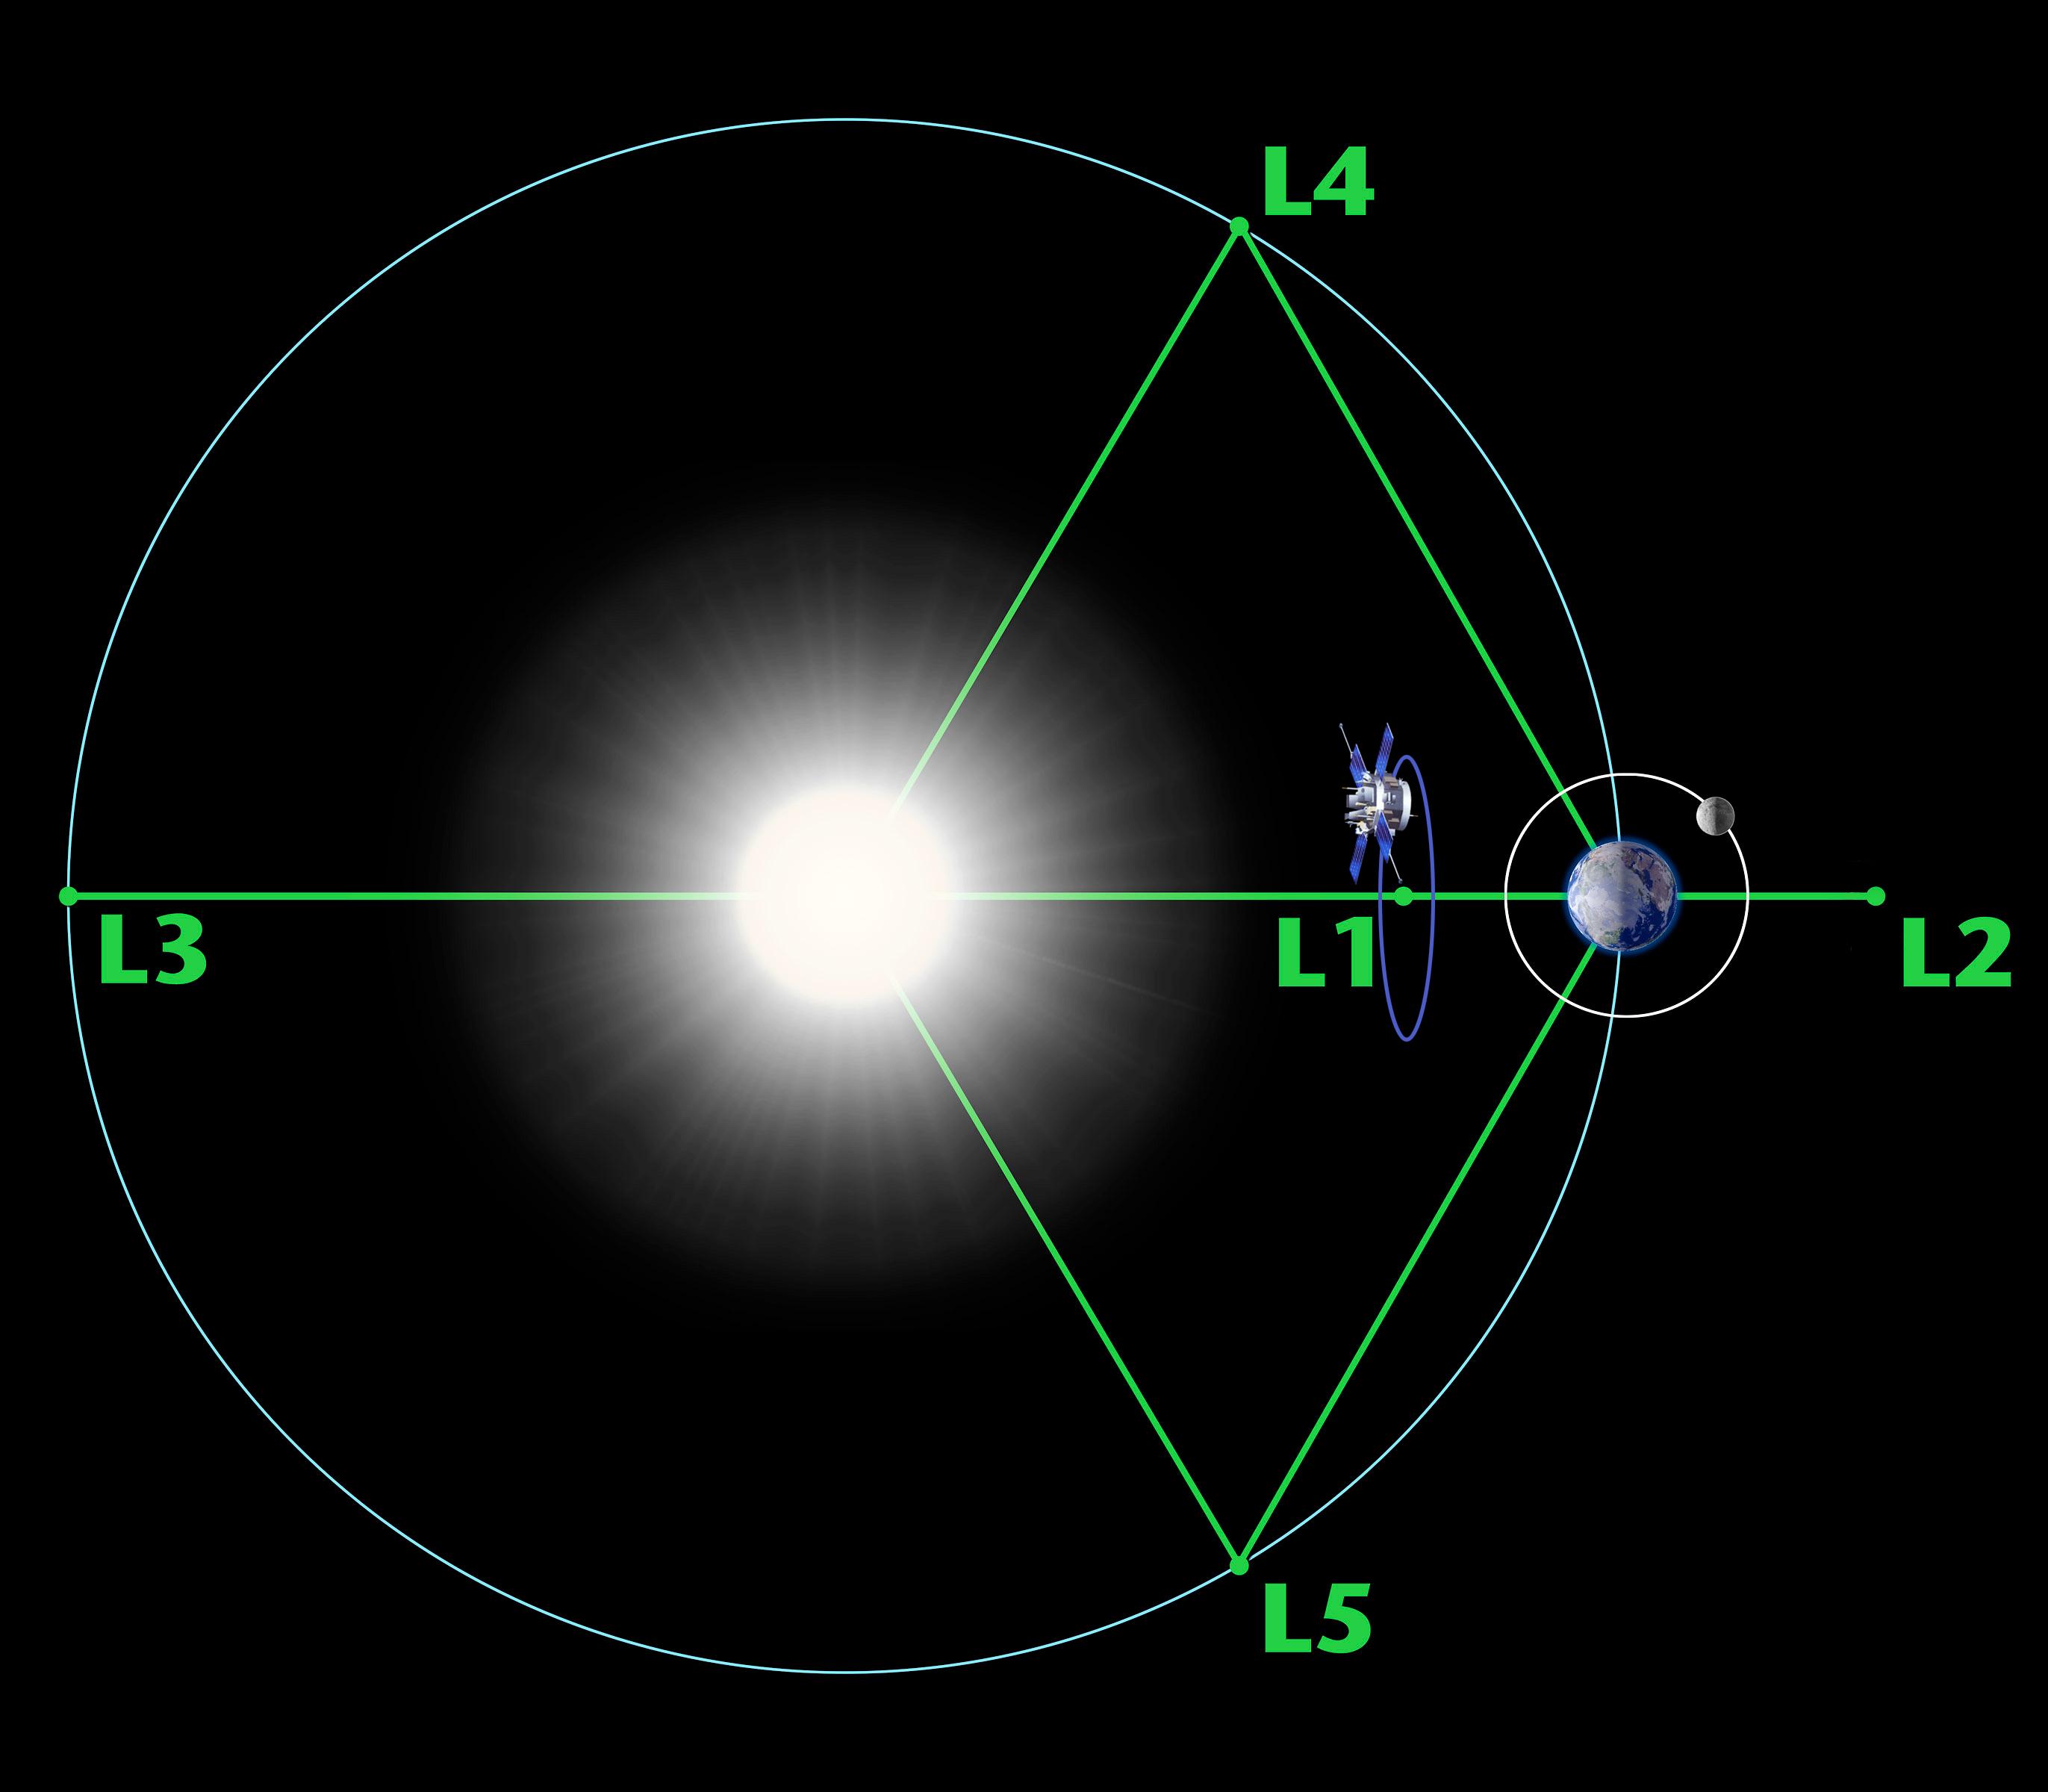
\includegraphics[scale=0.1]{images/LagrangePoints.jpg}
	\caption{The five Lagrange points (from NASA, \citeyear{Lagrange}).}
    \label{fig:LagrangePoints}
	\figSpace
\end{figure}
The uniqueness to the \textit{parameter variability} technique described previously is
that the data used as inputs into the models are not in-situ measurements from
the past, but are physically relevant artificial data that has meaning to the
space weather community. The CCMC allows for model runs to be configured using a
web interface; the run is submitted to staff who then execute the
model with the selected inputs and configuration. The input parameters are
submitted through a data file that contains values for $\mathbf{B^{IMF}}$,
$\mathbf{V}$, $\rho$, $T$. To determine the values to use as artificial inputs,
Advanced Composition Explorer (ACE) measurements were used because they
provide measurements from the solar wind taken from the L1 point ahead of Earth
in the Sun-to-Earth line over a full solar cycle, as shown in Figure
\ref{fig:LagrangePoints}. The in-situ data that was measured by instruments on
the ACE spacecraft were obtained from the OMNIWeb web site provided by the NASA
Goddard Space Flight Center (OMNIWeb, \citeyear{OMNIWeb}) between the dates of
January 1st, 2000 to January 1st, 2011.

\begin{figure}
	\centering
	\subfigure[Mean = 5.76 $cm^{-3}$, 80th and 20th Percentile = 11/2 $cm^{-3}$,
	95,128 Measurements]{
		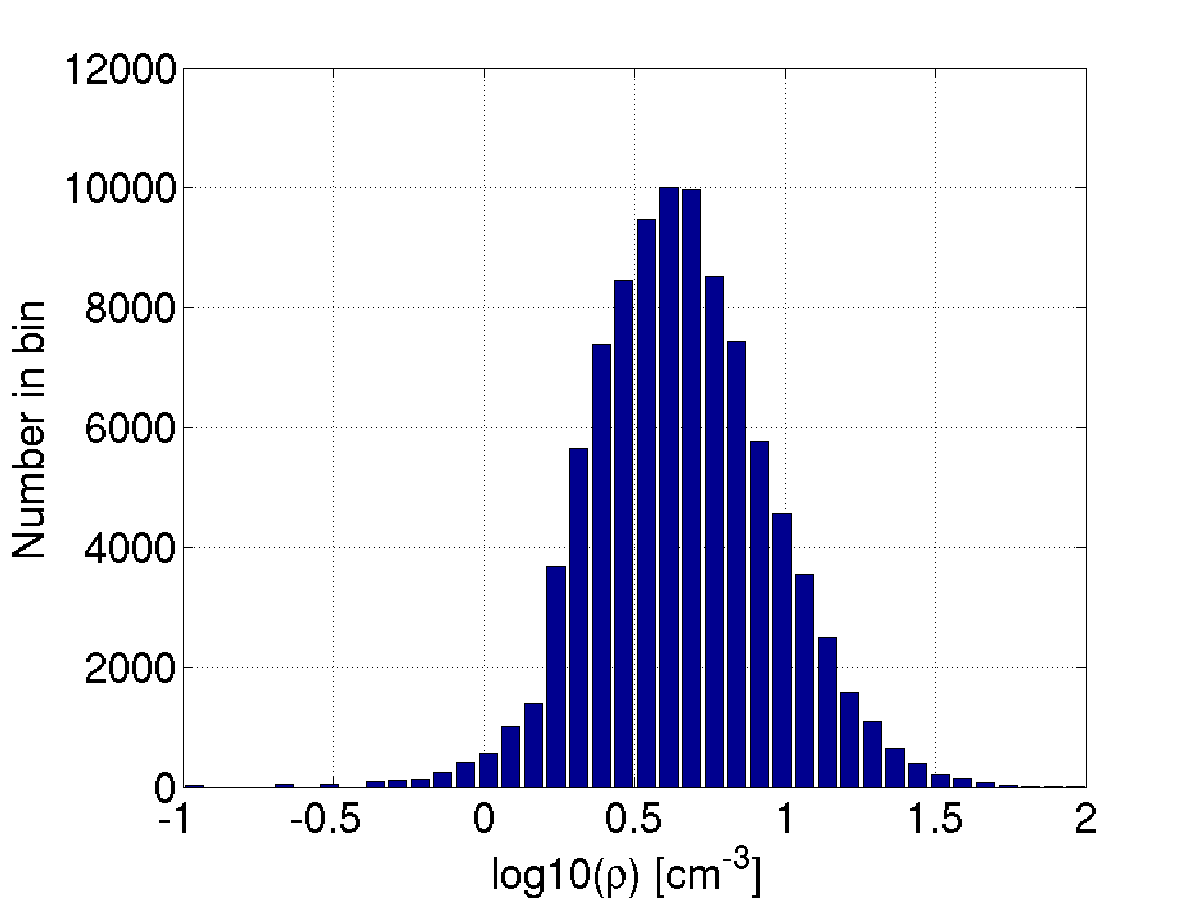
\includegraphics[scale=0.35]{images/hist_N.png}
	    \label{fig:hist_n}
	}\quad
	\subfigure[Mean = 101289 $K$, 80th and 20th Percentile = 217139/20554 $K$,
	95,255 Measurements]{
		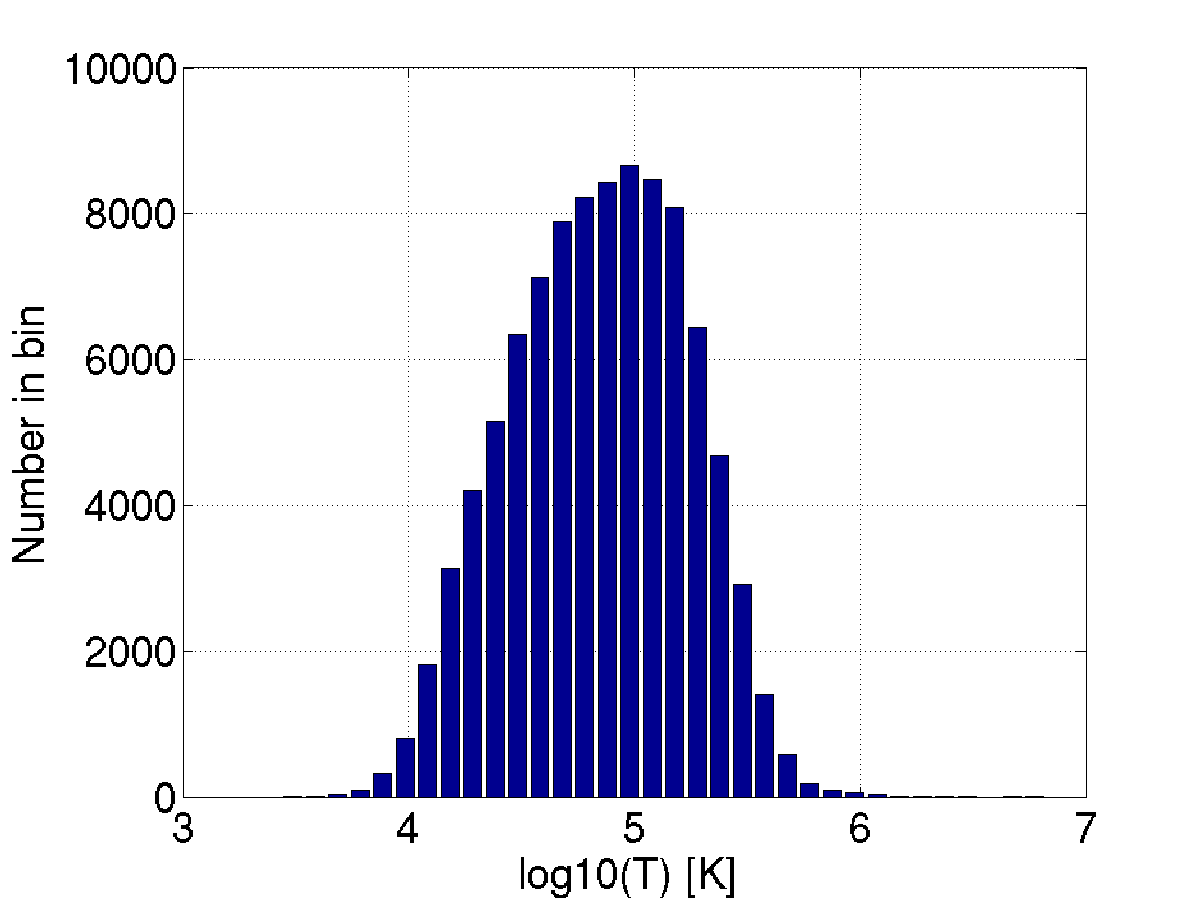
\includegraphics[scale=0.35]{images/hist_T.png}
	    \label{fig:hist_t}
	}\\
	\subfigure[Mean = 0.02 $nT$, 80th and 20th Percentile = 3.1/-3.0 $nT$, 96,417
	Measurements]{
		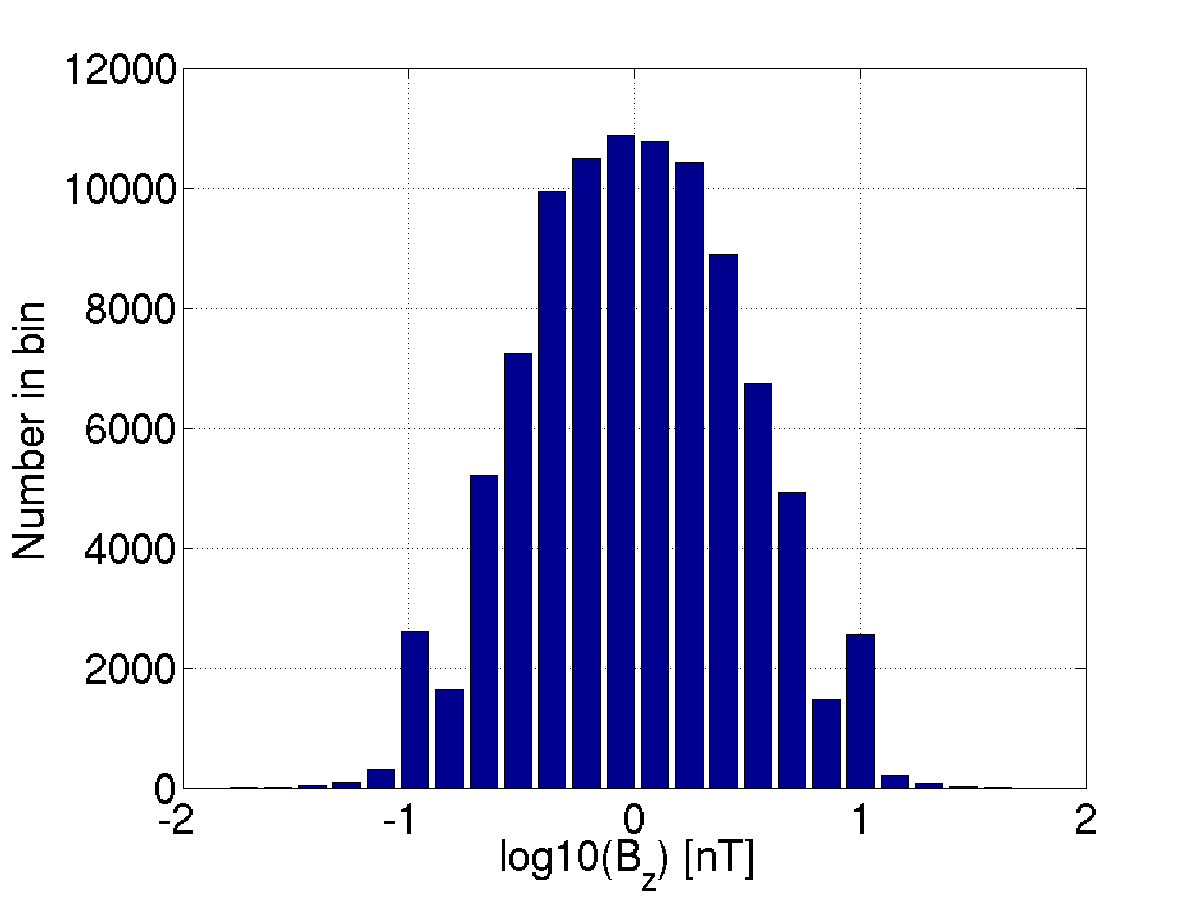
\includegraphics[scale=0.35]{images/hist_BZ.png}
	    \label{fig:hist_bz}
	}\quad
	\subfigure[Mean = 441.71 $km/s$, 80th and 20th Percentile = 604/320 $km/s$,
	96,311 Measurements]{
		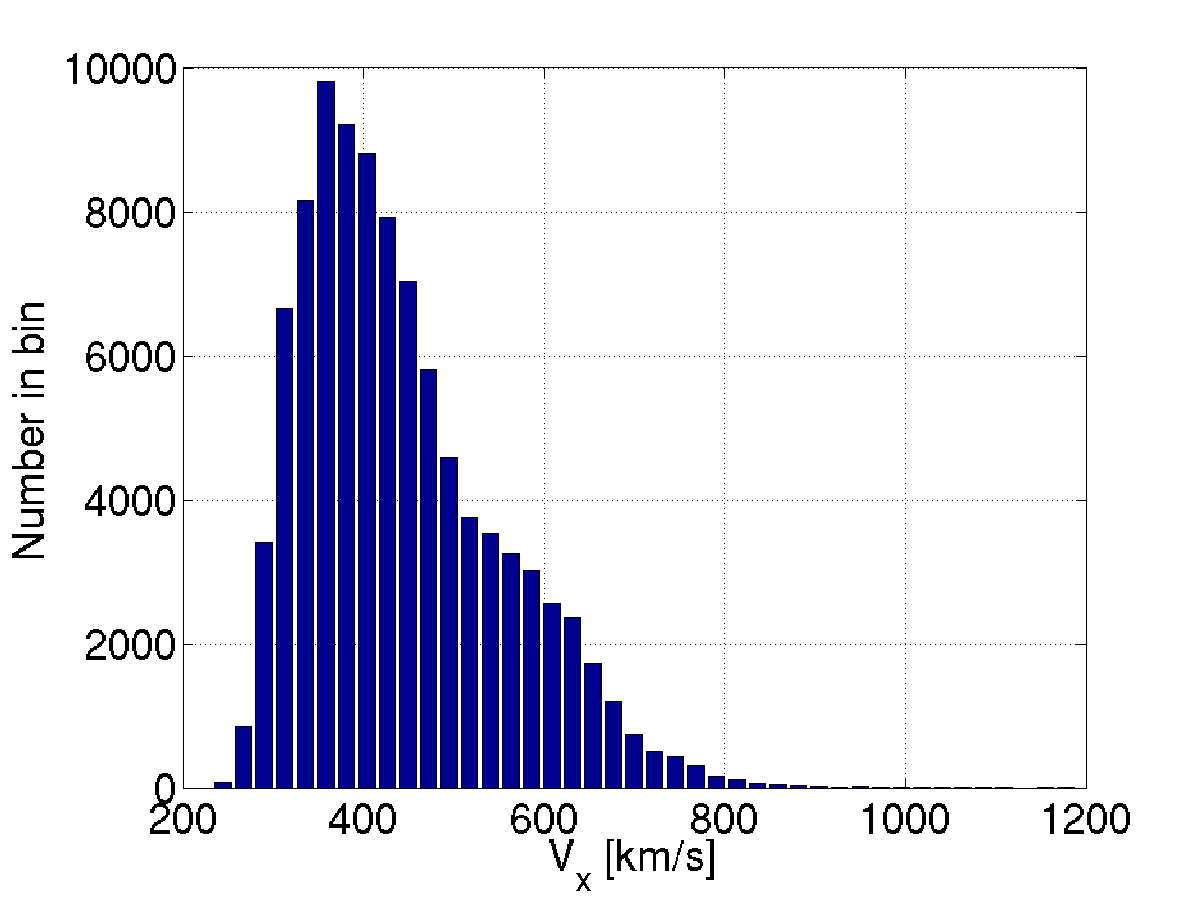
\includegraphics[scale=0.35]{images/hist_V.png}
	    \label{fig:hist_v}
    }
    \caption{Histogram of (a) $\rho$, (b) $T$, (c) $B_z^{IMF}$ and (d) $V_x$
    values measured by ACE, from January 1st, 2000 to January 1st, 2011. These
    histograms were used to determine appropriate values as artificial inputs to the models.}
	\figSpace
\end{figure}

MATLAB was used to read in the OMNIWeb data files, and histograms were created
for the solar wind variables. Figure \ref{fig:hist_n} is the histogram of solar
wind plasma density. The mean is 5.76 [$cm^{-3}$], the 80th percentile is 11
[$cm^{-3}$], and the 20th percentile is 2 [$cm^{-3}$]. Figure \ref{fig:hist_t}
is the histogram of solar wind temperature. The mean is 101289 [$K$], the 80th
percentile is 217139 [$K$] and the 20th percentile is 20554 [$K$]. Figure
\ref{fig:hist_bz} is the histogram of the solar wind interplanetary magnetic
field. The mean is 0.02 [$nT$], the 80th percentile is 3.1 [$nT$] and the 20th
percentile is -3.0 [$nT$]. Figure \ref{fig:hist_v} is the histogram of solar
wind velocity in the x direction, from Earth towards the Sun. The mean is 442 [$km/s$], the 80th percentile is 604 [$km/s$]
and the 20th percentile is 310 [$km/s$]. The 20th and 80th percentiles were used
for consistency with climatological values from in-situ data, specifically for
the experiment studying the effects of extreme solar wind conditions on the magnetosphere, higher and lower values for input
conditions are required to simulate high and low compression.
The percentile and mean values for each variable are displayed in Table
\ref{table:histtable}.

\begin{table}
\begin{center}
  \caption{ACE solar wind measurement histograms}
  \begin{tabular}{| l | c | c | c | }
    \hline
    \textbf{Variable} & \textbf{20th Percentile} & \textbf{Mean} &
    \textbf{80th Percentile} \\
    \hline $\rho$ [$cm^{-3}$] & 2 & 5.76  & 11   \\ \hline
    $T$ [$K$] & 20554 & 101289  & 217139 \\ \hline
    $V_x$ [$km/s$] & 310 & 442 & 604 \\ \hline
    $B_z$ [$nT$] & -3.0 & 0.02 & 3.1 \\ \hline
  \end{tabular}
  \label{table:histtable}
\end{center}
\end{table}

The simulations analyzed in this section used the input values shown in Table
\ref{table:run1}.

\begin{table}
\begin{center}
  \caption{Input parameters for $B_z^{IMF}$ reversal experiment}
  \begin{tabular}{| l | c | c | c | c | }
    \hline
    \textbf{$\rho$} [$cm^{-3}$] & \textbf{$T$} [$K$] &
    \textbf{$V_x$} [$km/s$] &
    \textbf{$B_z$} [$nT$]
    \\
    \hline 
    5.76 & 101289 & -442  & +3.1 to -3.0 at 00:30 \\ \hline
  \end{tabular}
  \label{table:run1}
\end{center}
\end{table}

\subsection{Results}

There are two different time periods in each run where the overall state of the
magnetosphere will significantly differ. First, the period of time before the
$B_z^{IMF}$ reversal occurs in which the magnetic field of the IMF is the same
direction as Earth's. Second, the period of time after the $B_z^{IMF}$ reversal
in which the direction of the IMF is opposite to that of Earth's. The reversal in $B_z^{IMF}$ occurs 30 minutes into each
run, the total time for each run was 6 hours. The changes expected are only due
to a reversal in $B_z^{IMF}$ direction and the differences between each model.

The grid used in the OpenGGCM model is different than that used in the BATS-R-US and SWMF models.
The stretched cartesian grid used in the OpenGGCM model has high resolutions in the
entire current sheet region and high resolutions near-Earth extending in the
Z and Y directions from the origin. The SAMR grid used in the BATS-R-US and SWMF models
has high resolution near-Earth and in the near-Earth current sheet region with
lower resolutions in the distant tail and distant northern and southern tail
lobes.

There are differences in how each model treats magnetospheric conditions
near-Earth (within 10$R_E$). The OpenGGCM and BATS-R-US models do not account
for particle drifts associated with the ring current. The SWMF model accounts
for particle drifts and the ring current.

The differences between the BATS-R-US and SWMF models are expected to be due to
the ring current. Based on Ampere's law, $\nabla \times \mathbf{B} =
\mu_0 \mathbf{J}$, the additions of a ring current should lead to an increase
of the z component of the magnetic field on the sunward side of the ring current
and decrease the z component of the magnetic field on the tailward side of
the ring current. This means the magnetic pressure is expected to be larger in
the sunward side of the ring current and smaller in the tailward side of the
ring current.

The magnetic pressure at the dayside magnetopause is effected by the reversal
from a positive $B_z^{IMF}$ direction to a negative $B_z^{IMF}$ direction. A
decrease in the magnetic pressure at that location will cause a movement of the
magnetopause towards Earth.

Figure \ref{fig:OpenGGCMatReversal} shows the OpenGGCM model output during the timeframe
where the magnetopause moves Earthward due
to a reduction in magnetic pressure, consistent with expectations. 
\begin{figure}
	\centering
	\subfigure{%
		\includegraphics[scale=0.36]{/mnt/Disk2/Brian_Curtis_042213_1/Results/images/Bz_File8.png}
		}
	\subfigure{%
		\includegraphics[scale=0.36]{/mnt/Disk2/Brian_Curtis_042213_1/Results/images/Bz_File9.png}
		}
	\subfigure{%
		\includegraphics[scale=0.36]{/mnt/Disk2/Brian_Curtis_042213_1/Results/images/Bz_File10.png}
		}
	\caption{OpenGGCM $B_z$ output shortly after the $B_z^{IMF}$ reversal.}
	\figSpace
	\label{fig:OpenGGCMatReversal}
\end{figure}

To better understand the differences in the position of the magnetopause
between the three models before and after the $B_z^{IMF}$ reversal,
model output difference images are used.

Figure \ref{fig:BdiffBeforeFlip} shows three comparisons between two models at a
time. The top image is a percent difference of $B_z$ between the OpenGGCM and
BATS-R-US models; the BATS-R-US model values are subtracted from the OpenGGCM model
values for each grid point on the interpolated grid and that result is
divided by their mean at that grid point. The middle image is a percent difference of $B_z$ between
the OpenGGCM and SWMF models. The bottom image is a percent difference of $B_z$
between the BATS-R-US and SWMF models. The top image of Figure \ref{fig:BdiffBeforeFlip}
shows large and negative percent differences near the location of the magnetopause. The negative value means that the second model in the top image, BATS-R-US, has
higher values. From this type of information, the model with the farthest and
closest magnetopause can be determined. Before the $B_z^{IMF}$ reversal the OpenGGCM model
magnetopause is closest to Earth and the SWMF model magnetopause is farthest
from Earth.
\begin{figure}
	\centering
	\subfigure{
		\includegraphics[scale=0.36]{/mnt/Disk2/Results/0_1/images/Bz_Diff_File1.png}
		}
	\subfigure{
		\includegraphics[scale=0.36]{/mnt/Disk2/Results/0_2/images/Bz_Diff_File1.png}
		}
	\subfigure{
		\includegraphics[scale=0.36]{/mnt/Disk2/Results/1_2/images/Bz_Diff_File1.png}
		}
	\caption{$B_z$ percent differences between the OpenGGCM and
	BATS-R-US models (top), the OpenGGCM and SWMF models (middle), and the BATS-R-US
	and SWMF models (bottom) 25 minutes before the $B_z^{IMF}$ reversal.}
	\figSpace
	\label{fig:BdiffBeforeFlip}
\end{figure}

The SWMF model has a slightly higher magnetic pressure near the magnetopause in
comparison to the BATS-R-US model, which can be explained by the effect that the ring
current has locally. The differences in current strength before the $B_z^{IMF}$
reversal are shown in Figure \ref{fig:JxRingCurrent}, where comparing the top
(BATS-R-US) and bottom (SWMF) images, the tail currents are lower with the SWMF
model. Earth has a ring current brought about by the motions of plasma
trapped in the near-Earth magnetosphere. This current, which lies between
4-7 $R_E$, induces its own magnetic field. The direction of its magnetic field 
in the near-Earth tail region opposes the direction of the field created by the current
sheet current, weakening it near-Earth. The direction of $B_z$ from the ring
current near the magnetopause is the same as the direction of Earth's magnetic
field and thus increases the magnetic pressure in that location. That increase
in magnetic pressure explains why the SWMF model magnetopause is farthest from
Earth, as shown in Figure \ref{fig:BdiffBeforeFlip}.

\begin{figure}
	\centering
	\subfigure{%
		\includegraphics[scale=0.36]{/mnt/Disk2/Brian_Curtis_042213_2/Results/images/Jx_File1.png}
		}
	\subfigure{%
		\includegraphics[scale=0.36]{/mnt/Disk2/Brian_Curtis_042213_3/Results/images/Jx_File1.png}
		}
	\caption{$J_x$ for BATS-R-US (top) and SWMF (bottom).}
	\figSpace
	\label{fig:JxRingCurrent}
\end{figure}

Figure \ref{fig:BdiffAfterFlip}, 60 minutes after the $B_z^{IMF}$ reversal, shows that
under negative $B_z^{IMF}$ conditions, the OpenGGCM model magnetopause is closest to
Earth and the BATS-R-US magnetopause is farthest from Earth.

\begin{figure}
	\centering
	\subfigure{
		\includegraphics[scale=0.36]{/mnt/Disk2/Results/0_1/images/Bz_Diff_File30.png}
		}
	\subfigure{
		\includegraphics[scale=0.36]{/mnt/Disk2/Results/0_2/images/Bz_Diff_File30.png}
		}
	\subfigure{
		\includegraphics[scale=0.36]{/mnt/Disk2/Results/1_2/images/Bz_Diff_File30.png}
		}
	\caption{$B_z$ Percent differences between the OpenGGCM and
	BATS-R-US models (top), the OpenGGCM and SWMF models (middle), and the
	BATS-R-US and SWMF models (bottom) 60 minutes after the $B_z^{IMF}$ reversal.}
	\figSpace
	\label{fig:BdiffAfterFlip}
\end{figure}

When plasma from the sun traveling at supersonic speeds interacts with the
magnetosphere, it eventually slows down below the speed of sound. This
transition from supersonic to subsonic causes a shock region ahead of the
magnetosphere, which is referred to as the bow shock. The velocity of the plasma
continues to decrease as it compresses and heats, leading to higher densities
between the magnetopause and the bow shock. Figure \ref{fig:rhoBeforeFlip} shows
this for all three models. There are higher densities in the current sheet that
are typically on the order of 0.1 to 1 $cm^{-3}$, but these values fit
in one color bin of the plots and are not visible.

Through various mechanisms, plasma can enter the magnetosphere cavity. Some of this plasma becomes
trapped on the closed magnetic field lines that surround Earth resulting in higher near-Earth densities.
The differences in densities seen near-Earth and in the tail region
between the models before the $B_z^{IMF}$ reversal are shown in Figure
\ref{fig:rhodiffBeforeFlip}. The larger differences seen in the magnetotail when
comparing the OpenGGCM model with the SWMF model
is due to the OpenGGCM model not accounting for the ring current. This
plot also shows that the SWMF model has highest densities in the current sheet
region.

\begin{figure}
	\centering
	\subfigure{%
		\includegraphics[scale=0.36]{/mnt/Disk2/Brian_Curtis_042213_1/Results/images/rho_File1.png}
		}
	\subfigure{%
		\includegraphics[scale=0.36]{/mnt/Disk2/Brian_Curtis_042213_2/Results/images/rho_File1.png}
		}
	\subfigure{%
		\includegraphics[scale=0.36]{/mnt/Disk2/Brian_Curtis_042213_3/Results/images/rho_File1.png}
		}
	\caption{$\rho$ for OpenGGCM (top) , BATS-R-US (middle), and SWMF (bottom) 25
	minutes before the $B_z^{IMF}$ reversal.}
	\figSpace
	\label{fig:rhoBeforeFlip}
\end{figure}

\begin{figure}
	\centering
	\subfigure{
		\includegraphics[scale=0.36]{/mnt/Disk2/Results/0_1/images/rho_Diff_File1.png}
		}
	\subfigure{
		\includegraphics[scale=0.36]{/mnt/Disk2/Results/0_2/images/rho_Diff_File1.png}
		}
	\subfigure{
		\includegraphics[scale=0.36]{/mnt/Disk2/Results/1_2/images/rho_Diff_File1.png}
		}
	\caption{$\rho$ Percent differences between the OpenGGCM and
	the BATS-R-US models (top), the OpenGGCM and SWMF models (middle), and the
	BATS-R-US and SWMF models (bottom) 25 minutes before the $B_z^{IMF}$ reversal.}
	\figSpace
	\label{fig:rhodiffBeforeFlip}
\end{figure}

After the $B_z^{IMF}$ reversal, shown in Figure \ref{fig:rhodiffAfterFlip}, the
OpenGGCM densities in the distant current sheet become higher than the
BATS-R-US. The SWMF model still has higher densities in the current sheet, which
is shown in the third image that compares the BATS-R-US and SWMF models (where
there are darker blue colors in the current sheet).

\begin{figure}
	\centering
	\subfigure{
		\includegraphics[scale=0.36]{/mnt/Disk2/Results/0_1/images/rho_Diff_File45.png}
		}
	\subfigure{
		\includegraphics[scale=0.36]{/mnt/Disk2/Results/0_2/images/rho_Diff_File45.png}
		}
	\subfigure{
		\includegraphics[scale=0.36]{/mnt/Disk2/Results/1_2/images/rho_Diff_File45.png}
		}
	\caption{$\rho$ Percent differences between the OpenGGCM and
	BATS-R-US models (top), the OpenGGCM and SWMF models (middle), and the
	BATS-R-US and SWMF models (bottom) 115 minutes after the $B_z^{IMF}$ reversal.}
	\figSpace
	\label{fig:rhodiffAfterFlip}
\end{figure}

As noted previously, and shown in Figure \ref{fig:UxBeforeFlip}, the solar wind
$U_x$ slows down from a supersonic to a subsonic speed which causes a shock.
$U_x$ is then reduced more as its distance from Earth decreases.
The current sheet is formed from two opposing magnetic field directions close to
one another, which is caused by the stretching in the
magnetotail. In this region there is a near-zero $B_z$, which allows for
reconnection. This reconnection transports particles in the current sheet region
both tailward and Earthward. The velocities seen in the current sheet region in
all models are consistent with this.
\begin{figure}
	\centering
	\subfigure{%
		\includegraphics[scale=0.36]{/mnt/Disk2/Brian_Curtis_042213_1/Results/images/Ux_File1.png}
		}
	\subfigure{%
		\includegraphics[scale=0.36]{/mnt/Disk2/Brian_Curtis_042213_2/Results/images/Ux_File1.png}
		}
	\subfigure{%
		\includegraphics[scale=0.36]{/mnt/Disk2/Brian_Curtis_042213_3/Results/images/Ux_File1.png}
		}
	\caption{$U_x$ for OpenGGCM (top), BATS-R-US (middle), and SWMF (bottom) 25
	minutes before the $B_z^{IMF}$ reversal.}
	\figSpace
	\label{fig:UxBeforeFlip}
\end{figure}

Before the $B_z^{IMF}$ reversal, Figure \ref{fig:UxdiffBeforeFlip} shows that the
OpenGGCM model has higher $U_x$ in the distant tail current sheet compared to
the BATS-R-US model and the SWMF model. The near-Earth current sheet velocities
are higher in the BATS-R-US model and the SWMF model than the OpenGGCM model. In
comparison, the BATS-R-US model and the SWMF model comparison (bottom), shows
that the SWMF model has higher $U_x$ in the near-Earth current sheet and the
BATS-R-US model has higher $U_x$ in the distant tail.
\begin{figure}
	\centering
	\subfigure{
		\includegraphics[scale=0.36]{/mnt/Disk2/Results/0_1/images/Ux_Diff_File1.png}
		}
	\subfigure{
		\includegraphics[scale=0.36]{/mnt/Disk2/Results/0_2/images/Ux_Diff_File1.png}
		}
	\subfigure{
		\includegraphics[scale=0.36]{/mnt/Disk2/Results/1_2/images/Ux_Diff_File1.png}
		}
	\caption{$U_x$ percent differences between OpenGGCM and
	BATS-R-US (top), OpenGGCM and SWMF (middle), and BATS-R-US and SWMF (bottom)
	25 minutes before the $B_z^{IMF}$ reversal.}
	\figSpace
	\label{fig:UxdiffBeforeFlip}
\end{figure}

After the $B_z^{IMF}$ reversal, Figure \ref{fig:UxdiffAfterFlip} shows the
BATS-R-US model has higher $U_x$ compared to the OpenGGCM model in the current
sheet region (top), while the OpenGGCM model compared to the SWMF model (middle)
shows higher $U_x$ in the current sheet region for the OpenGGCM model and higher
$U_x$ in the north and south tail lobes outside of the current sheet region for
the SWMF model. Comparing the BATS-R-US model and the SWMF model (bottom), the
BATS-R-US model has higher $U_x$ in the current sheet region.
\begin{figure}
	\centering
	\subfigure{
		\includegraphics[scale=0.36]{/mnt/Disk2/Results/0_1/images/Ux_Diff_File31.png}
		}
	\subfigure{
		\includegraphics[scale=0.36]{/mnt/Disk2/Results/0_2/images/Ux_Diff_File31.png}
		}
	\subfigure{
		\includegraphics[scale=0.36]{/mnt/Disk2/Results/1_2/images/Ux_Diff_File31.png}
		}
	\caption{$U_x$ percent differences between OpenGGCM and
	BATS-R-US (top), OpenGGCM and SWMF (middle), and BATS-R-US and SWMF (bottom)
	85 minutes after the $B_z^{IMF}$ reversal.}
	\figSpace
	\label{fig:UxdiffAfterFlip}
\end{figure}

\subsection{Discussion and Conclusions}

The position of the magnetopause and shape of the magnetosphere are
determined by the magnetic field of Earth and its interaction with the
solar wind. The OpenGGCM model, which did not account for a
near-Earth ring-current, has the weakest magnetic pressure and therefore the
closest magnetopause to Earth of the three models. The model-predicted position
of the magnetopause is important for forecasters because they need to be able to tell companies with
space-based technologies, especially those in geosynchronous orbit, if their
equipment may be effected by the plasma that comes from the solar
wind.

\cite{Garcia2007} discuss how the absence of the ring current in the Lyon
Fedder Mobarry (LFM) magnetospheric model compares to magnetopause location
measurements made by satellites. They found that an insufficient ring current would not push the
magnetopause far enough Sunward. The ring current effect on the magnetopause
location is evident with this experiment as well.

The models show the slowdown of $U_x$ Earthward of the
bow shock, and inside the magnetosphere. The velocities in the current sheet
region are important to forecasters as to the timing of storms impacts seen at
Earth. Reconnection is tied to the
$U_x$ such that a faster reconnection will yield faster velocities and a slower
reconnection will yield slower velocities.

Model output differences can give model developers a better view of
the differences between their model and other models for similar regions in
space. With model runs involving in-situ data, the space weather community is
already doing a lot of analysis into determining which model is better for
select events.

\subsubsection{Summary}
For a reversal in $B_z^{IMF}$, the
following occur in the models:
\begin{itemize}
  \item The OpenGGCM model magnetopause is closest to Earth as it has the weakest
  near-Earth magnetic pressure.
  \item Under positive $B_z^{IMF}$ conditions, the ring current pushes the SWMF
  model magnetopause farther sunward than that in the BATS-R-US model.
  \item Under negative $B_z^{IMF}$ conditions, the SWMF model magnetopause is
  farther Earthward than that in the BATS-R-US model.
  \item The differences in magnetopause positions between BATS-R-US and SWMF
  are due to the effects of the ring current addition to the SWMF model.
  \item Densities are highest with the SWMF model and lowest with the OpenGGCM
  model.
  \item The OpenGGCM model tail currents are significantly different from the
  BATS-R-US model and SWMF at over 100 percent differences.
\end{itemize}


\section[Preconditioning]{The influence of preconditioning on MHD magnetospheric
models} This section addresses the influence of the amount of time spent on preconditioning
on magnetospheric MHD models. There are examples of previous research dealing
with magnetospheric preconditioning as described in the following section, but
the term preconditioning used here has a slightly different meaning as
described previously in Section \ref{InitialConditions}. In order to perform a
\textit{parameter variability - sensitivity validation}, it is necessary to be able to
control input into the model, and for consistency, there is a necessity to keep
as many of the inputs constant.

\subsection{Background}
\citet{Lavraud2006} performed a study on the state of the magnetosphere for a
subset of coronal mass ejection and co-rotating interaction region events and
looked to identify if there was a preconditioning effect for sustained northward
interplanetary magnetic fields (IMF). The study aimed to test a hypothesis that
a cold dense plasma sheet prior to storm initiation, which is known to enhance the
ring current, is caused by a sustained northward IMF. The enhancement of the
ring current would lead to lower storm-time $D_{st}$ values. Measured and
modeled $D_{st}$ values were compared with that of a semi-empirical $D_{st}$
model. The modeled $D_{st}$ tended to underestimate the actual measured $D_{st}$
during events where there was a sustained northward IMF before the start of a
storm. Plasma data from Los Alamos satellites were consistent with a colder and
denser plasma sheet being present for the events in which a sustained northward
IMF was present prior to storm initiation. A follow up study by
\cite{Weigel2010} showed that there was no statistically significant
preconditioning effect as claimed.

\citet{Juusola2013} considered how the ring current plays a role in steady
magnetospheric convection (SMC). SMC occurs when there is a balance of
reconnection rates on the dayside and in the distant tail region. This study
showed that the ring current strength needed to be at a specific level, no
higher and no lower, in order for SMC to occur. Through a study of $B_z^{IMF}$ and
$V_x$ along with the SYM-H index, \citet{Juusola2013} determined that most SMC events are
preconditioned with low $V_x$ and a slightly negative $B_z^{IMF}$, which provides
energy to the ring current and prevents bursty convection from occurring, thus
allowing a continuous SMC event.

\subsection{Motivation}
The preconditioning described by \citet{Lavraud2006} involved the condition of
the magnetosphere prior to a storm that would cause lower $D_{st}$ values during the storm. The preconditioning
described by \citet{Juusola2013} uses the term preconditioning as a set of specific
conditions that must be met in order for SMC events to occur. The term
preconditioning used in these papers involves an actual state that the
magnetosphere needs to be in at or prior to an event. Magnetospheric models are
started with artificial initial conditions and then run for a certain amount of
time prior to actual or user provided data being used as boundary conditions.
The preconditioning considered in this thesis involves the amount of time
between the start of the run and the time of an event versus the state of the solar wind or
magnetospheric variables prior to an event.

According to \citet{Raeder2003} and \citet{Buchner2003}, the magnetosphere will
form within one hour from the start of preconditioning in a MHD simulation.
According to \cite{Raeder1999}, the initial conditions for the OpenGGCM model magnetic field
are started from the superposition of Earth's dipole with a mirror dipole that
is equally as strong, such that $B_x$ is zero in the $x = 16R_E$ plane.
Sunward of $x = 16R_E$, the $B$ field in this plane is replaced by the initial
solar wind field and the run is started. \citet{Buchner2003} presented a question to the
community when discussing the length of preconditioning time used in magnetospheric MHD models and noted that because the magnetosphere has a long memory from previous
conditions, it may take a few hours of preconditioning time to stabilize
the magnetosphere.  However,
there has been no published research on the appropriate amount of time or the influence of the preconditioning time on model predictions.

\subsection{Methodology}
The methodology used in this section is similar to the methodology for the $B_z^{IMF}$ reversal experiment described in section
\ref{SimilarMethodology}. 

\begin{figure}
	\begin{centering}
	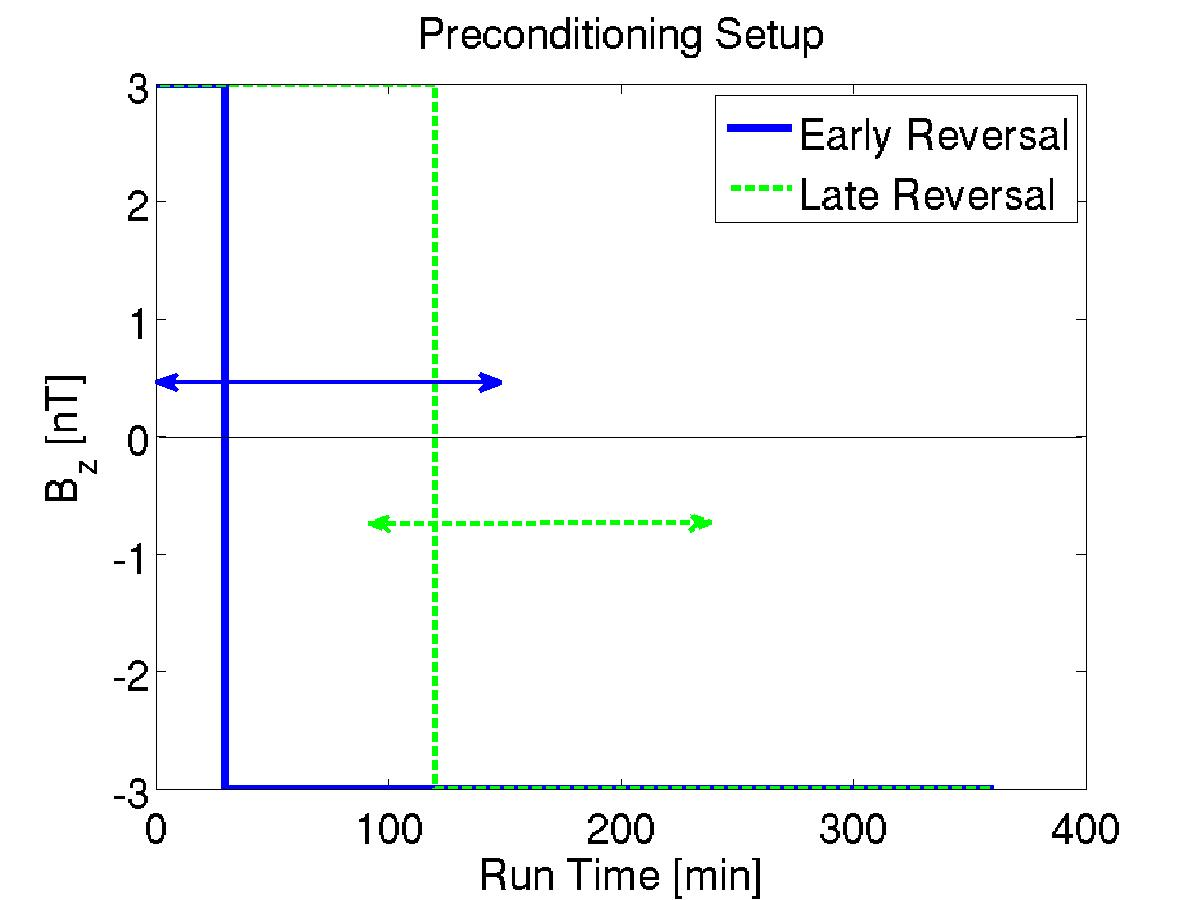
\includegraphics[scale=0.35]{images/PreconditionSetup.jpg}
	\caption{Setup for the preconditioning experiment. Two equal length time
	intervals from each run with the reversal starting at 30 minutes into the start
	of the interval.}
	\label{fig:PreconditionSetup}
	\end{centering}
	\figSpace
\end{figure}

To evaluate the differences between the two models with a time-shifted
$B_z^{IMF}$ reversal, the output data from the two models were taken between 30
minutes before the reversal to 2 hours after the reversal, as shown in Figure
\ref{fig:PreconditionSetup}, and then inserted into the code that creates the
difference output, which was then processed by a Paraview Python code that
creates images.

\begin{table}
\begin{center}
  \caption{Input parameters for preconditioning experiment}
  \begin{tabular}{| l | c | c | c | c | }
    \hline
    \textbf{Run Num.} & \textbf{$\rho$} [$cm^{-3}$] & \textbf{$T$} [$K$] &
    \textbf{$U_x$} [$km/s$] &
    \textbf{$B_z$} [$nT$]
    \\
    \hline 
    1 & 5.76 & 101289 & -442  & +3.1 to -3.0 at 00:30 \\ \hline
    2 & 5.76 & 101289 & -442  & +3.1 to -3.0 at 02:00 \\ \hline
  \end{tabular}
  \label{table:runs12}
\end{center}
\end{table}

As shown in Table \ref{table:runs12} for run 1, $T$, $U_x$, and $\rho$ were kept
constant throughout the entire run. The only difference between the two runs is
the time at which $B_z^{IMF}$ was reversed from a positive to negative value.
This is physically meaningful as a $B_z^{IMF}$ reversal is a typical cause for enhanced
magnetospheric activity.

\subsection{Results}	
% B%
In Figure \ref{fig:BdiffPCBeforeFlip}, the top comparison is between the early
and late reversal runs for the OpenGGCM model. Red indicates locations where
the early reversal has higher values, while blue indicates locations where the
late reversal has higher values. The OpenGGCM model $B_z$ output shows
differences in the positioning of the entire magnetopause with the late reversal
having a magnetopause that is farther Sunward. There are also differences in the
current sheet region with neither the early or late reversal showing
consistently higher or lower values in one specific region of the current sheet.
The BATS-R-US and SWMF models show differences in the current sheet region
between $\pm$ 20 $R_E$ in the z direction.

\begin{figure}
	\centering
	\subfigure{
		\includegraphics[scale=0.36]{/mnt/Disk2/Precondition/Results/0_3/images/Bz_Diff_File1.png}
		}
	\subfigure{
		\includegraphics[scale=0.36]{/mnt/Disk2/Precondition/Results/1_4/images/Bz_Diff_File1.png}
		}
	\subfigure{
		\includegraphics[scale=0.36]{/mnt/Disk2/Precondition/Results/2_5/images/Bz_Diff_File1.png}
		}
	\caption{$B_z$ percent differences between the OpenGGCM model early and late
	reversals (top), BATS-R-US early and late reversals (middle), and SWMF early
	and late reversals (bottom) 25 minutes before the $B_z^{IMF}$ reversal.}
	\figSpace
	\label{fig:BdiffPCBeforeFlip}
\end{figure}

After the $B_z^{IMF}$ reversal, towards the end of the run, there are still
differences in the OpenGGCM model (top) run, while there are minimal to no
differences in the BATS-R-US model (middle) and the SWMF model (bottom) run, as
shown in Figure \ref{fig:BdiffPCAfterFlip}. The differences shown for the OpenGGCM model have
decreased near the magnetopause, but are still large in the current sheet
region.

\begin{figure}
	\centering
	\subfigure{
		\includegraphics[scale=0.36]{/mnt/Disk2/Precondition/Results/0_3/images/Bz_Diff_File26.png}
		}
	\subfigure{
		\includegraphics[scale=0.36]{/mnt/Disk2/Precondition/Results/1_4/images/Bz_Diff_File26.png}
		}
	\subfigure{
		\includegraphics[scale=0.36]{/mnt/Disk2/Precondition/Results/2_5/images/Bz_Diff_File26.png}
		}
	\caption{$B_z$ percent differences between the OpenGGCM model early and late
	reversals (top), BATS-R-US early and late reversals (middle), and SWMF early
	and late reversals (bottom) 60 minutes after the $B_z^{IMF}$ reversal. }
	\figSpace
	\label{fig:BdiffPCAfterFlip}
\end{figure}

% RHO%
In Figure \ref{fig:rhodiffPCBeforeFlip}, the largest differences occur in the
current sheet regions. The OpenGGCM model differences do not extend far
tailward within $\pm$10 $R_E$ in the z direction. The differences in both the BATS-R-US and
SWMF models are highest in the current sheet region and extend into the distant
tail within $\pm$20 $R_E$ in the z direction. In the BATS-R-US model runs, the early
reversal has higher values in the near-Earth current sheet region. In the
SWMF model, the early reversal has higher values nearest Earth outside of the
current sheet region. There are lower values for the late reversal in the
distant tail region.
\begin{figure}
	\centering
	\subfigure{
		\includegraphics[scale=0.36]{/mnt/Disk2/Precondition/Results/0_3/images/rho_Diff_File1.png}
		}
	\subfigure{
		\includegraphics[scale=0.36]{/mnt/Disk2/Precondition/Results/1_4/images/rho_Diff_File1.png}
		}
	\subfigure{
		\includegraphics[scale=0.36]{/mnt/Disk2/Precondition/Results/2_5/images/rho_Diff_File1.png}
		}
	\caption{$\rho$ percent differences between the OpenGGCM model early and late
	reversals (top), BATS-R-US early and late reversals (middle), and SWMF early
	and late reversals (bottom) 25 minutes before the $B_z^{IMF}$ reversal.}
	\figSpace
	\label{fig:rhodiffPCBeforeFlip}
\end{figure}

After the $B_z^{IMF}$ reversal, as shown in Figure \ref{fig:rhodiffPCAfterFlip}, 
there are only small regions of differences in the OpenGGCM model (top). The SWMF
model (bottom), and the BATS-R-US model (middle), have near zero differences.
\begin{figure}
	\centering
	\subfigure{
		\includegraphics[scale=0.36]{/mnt/Disk2/Precondition/Results/0_3/images/rho_Diff_File26.png}
		}
	\subfigure{
		\includegraphics[scale=0.36]{/mnt/Disk2/Precondition/Results/1_4/images/rho_Diff_File26.png}
		}
	\subfigure{
		\includegraphics[scale=0.36]{/mnt/Disk2/Precondition/Results/2_5/images/rho_Diff_File26.png}
		}
	\caption{$\rho$ percent differences between the OpenGGCM model early and late
	reversals (top), BATS-R-US early and late reversals (middle), and SWMF early
	and late reversals (bottom) 60 minutes after the $B_z^{IMF}$ reversal.}
	\figSpace
	\label{fig:rhodiffPCAfterFlip}
\end{figure}

% U_x%
The $U_x$ plots in Figure \ref{fig:UxdiffPCBeforeFlip} show the highest
differences in the current sheet region for all three models.
No one run has higher differences in which the opposite run does
not. The regions in which one run has higher values over the other is not
consistent. The BATS-R-US model (middle) late reversal has highest values in the
current sheet region. The SWMF model (bottom) has highest differences with the
late reversal run in the north and south hemispheres of the magnetosphere outside of
the current sheet region and far from Earth, while the early reversal has higher values
close to Earth.
\begin{figure}
	\centering
	\subfigure{
		\includegraphics[scale=0.36]{/mnt/Disk2/Precondition/Results/0_3/images/Ux_Diff_File1.png}
		}
	\subfigure{
		\includegraphics[scale=0.36]{/mnt/Disk2/Precondition/Results/1_4/images/Ux_Diff_File1.png}
		}
	\subfigure{
		\includegraphics[scale=0.36]{/mnt/Disk2/Precondition/Results/2_5/images/Ux_Diff_File1.png}
		}
	\caption{$\rho$ percent differences between the OpenGGCM model early and late
	reversals (top), BATS-R-US early and late reversals (middle), and SWMF early
	and late reversals (bottom) 25 minutes before the $B_z^{IMF}$ reversal.}
	\figSpace
	\label{fig:UxdiffPCBeforeFlip}
\end{figure}

After the $B_z^{IMF}$ reversal, as shown in Figure \ref{fig:UxdiffPCAfterFlip}, most
of the OpenGGCM model (top) differences are in the current sheet region. The early
reversal has higher values tailward of -40$R_E$, while the late reversal has higher
values Earthward of -40$R_E$.
\begin{figure}
	\centering
	\subfigure{
		\includegraphics[scale=0.36]{/mnt/Disk2/Precondition/Results/0_3/images/Ux_Diff_File26.png}
		}
	\subfigure{
		\includegraphics[scale=0.36]{/mnt/Disk2/Precondition/Results/1_4/images/Ux_Diff_File26.png}
		}
	\subfigure{
		\includegraphics[scale=0.36]{/mnt/Disk2/Precondition/Results/2_5/images/Ux_Diff_File26.png}
		}
	\caption{$\rho$ percent differences between the OpenGGCM model early and late
	reversals (top), BATS-R-US early and late reversals (middle), and SWMF early
	and late reversals (bottom) 60 minutes after the $B_z^{IMF}$ reversal.}
	\figSpace
	\label{fig:UxdiffPCAfterFlip}
\end{figure}

\subsection{Discussion and Conclusions}
The differences in the magnetopause position, for
all three models, are of concern to forecasters. If there is any risk of
the magnetopause traveling farther towards Earth than geosynchronous orbit, then the companies
that control space based technology may need to take action to protect their
equipment from plasma in the solar wind.

The differences seen with all three models, for all three scalar plots, before
the $B_z^{IMF}$ reversal, show that under northward IMF conditions, the model output depends strongly on preconditioning time. With a different output from the same model, there
is an expectation that this would change the effects that the $B_z^{IMF}$ reversal has
on each model under non-artificial conditions. This preconditioning result is similar to results seen with each event validity
validation done where each result is different because the conditions before
$B_z^{IMF}$ reversals were different, as seen in a study by \citet{Juusola2013}.

After the $B_z^{IMF}$ reversal, all three models had smaller differences. The BATS-R-US and SWMF
models both show a decrease of difference to near zero percent. The OpenGGCM
model was the exception in the current sheet region.

In determining if these models had enough preconditioning, the evidence from
this research shows a significant sensitivity to preconditioning time before the
$B_z^{IMF}$ reversal and much smaller differences after the $B_z^{IMF}$
reversal.

\subsubsection{Summary}
\begin{itemize}
  \item Longer preconditioning time allowed the magnetosphere to relax more
  giving different positions for the magnetopause with all three models.
  \item The OpenGGCM model magnetopause position differences were larger than
  that of SWMF or BATS-R-US.
  \item There were large differences for all three models before the $B_z^{IMF}$
  reversal.
  \item The differences in the current sheet region for the OpenGGCM model were similar before and after the reversal.
  \item The BATS-R-US and SWMF model differences decreased after the $B_z^{IMF}$
  reversal to near zero.
\end{itemize}
\section[Extreme Conditions]{Extreme conditions in the magnetosphere}

\subsection{Background and Motivation}
In order to improve predictability of the magnetopause location under extreme
events, \citet{Shue1998} took magnetopause crossing satellite measurements and
compared them to two models. The first model (\textit{Petrinic and Russell},
1996) was compared to the \textit{Shue et. al.} (1997) model. Both models
compared well with the magnetopause crossings at the day-side magnetopause,
while the \textit{Shue et. al.} (1997) model had a poorer fit for magnetopause
crossings at the flanks.
The explanation for the discrepancies was that they were ``due to the inappropriate linear extrapolation from the parameter range for average solar wind conditions to that
for extreme conditions''. Upon correction, the \textit{Shue et. al.}
(1997) model was able to better predict magnetopause flank crossings.

Companies and government agencies with space-based assests are interested in the
duration of extreme storms. \citet{Cid2013} studied the effectiveness of a
hyperbolic function for estimating the decay time after minimum $D_{st}$ values
for extreme storms.
A hyperbolic function was used because previously used linear functions did not
accurately predict the the decay time of extreme storms. The extremity of the
storm was determined by the $D_{st}$ index where data was available, and a
``Local Disturbance Index'' taken from the $H$ component of geomagnetic field
measured at each observatory where $D_{st}$ data was not available.

Extreme space weather events are an active area of research.  For
example, statistical analysis on the long range correlations was by
\citet{Sharma2011} used a database of over 5 million events. The basis
for the research was that dynamical and statistical features in
extreme events are complicated due to the turbulent nature of the
solar wind.  An auto-correlation function and a detrended fluctuation
analysis were performed to find the long-range correlations.  In this
work, the extreme events were compiled from a
database. Although the used data was not model--based and the approach involved examining statistical properties, it did not involve a comparison to other models.
By comparing multiple models given the same generic input, as done in this experiment, along
with the extremes of input variables, forecasters may gain a better
understanding of which model is best to use for a variety of extreme
space weather conditions.

%\subsection{Motivation}
%Two of the validation techniques described by \citet{Sargent2004},
%\textit{comparison to other models}, and \textit{parameter variability} were us%ed in this section to better understand model behavior under extreme conditions.
%\citet{Cid2013} compared both a hyperbolic and linear fit to recovery times of
%strong geomagnetic storms to determine which provided the best comparison. The
%study determined that the hyperbolic fit was the best match for strong storms,
%and as the storm intensity decreased a linear approach became the better choice%.
%This study uses a \textit{historical data} validation.

\subsection{Methodology}
The similarities of the methodologies in all three experiments are described in
the methodology section for the $B_z^{IMF}$ reversal experiment in section
\ref{SimilarMethodology} of this dissertation. 

\begin{table}
\begin{center}
  \caption{Input parameters for extreme conditions experiment}
  \begin{tabular}{| l | c | c | c | c | }
    \hline
    \textbf{Run Num.} & \textbf{$\rho$} & \textbf{$T$} & \textbf{$Vx$} &
    \textbf{$B_z$}
    \\
    \hline 
    3 & 11 & 101289 & -604  & -3.0 \\ \hline
    4 & 2 & 101289 & -320  & 3.1 \\ \hline
  \end{tabular}
  \label{table:runs34}
\end{center}
\end{table}
As shown in Table \ref{table:runs34}, in order to compress the magnetosphere,
input variables were chosen corresponding to a high solar wind velocity, a negative
solar wind magnetic field, and a high solar wind density. Under high
compression, magnetospheric features may be difficult to resolve due to limitations in resolution.  For the low compression run, input variables were chosen that lead to a small
compression of the magnetosphere: a low solar wind velocity, a positive $B_z$,
and a low density.

\subsection{Results}
\subsubsection{High Magnetospheric Compression}
% B%
As shown in Figure \ref{fig:BHighCompressionBeginning}, all three models have
similar $B_z$ contours. The OpenGGCM model magnetopause is closest to Earth.
In Figure \ref{fig:BDiffHighBeginning}, the BATS-R-US model magnetopause is
shown to be farther Sunward than that for the SWMF model. Figure
\ref{fig:BDiffHighBeginning} also shows higher $B_z$ values
to occur in the tail region for the BATS-R-US and SWMF models.

\begin{figure}
	\centering
	\subfigure{%
		\includegraphics[scale=0.36]{/mnt/Disk2/Brian_Curtis_042413_1/Results/images/Bz_File9.png}
		}
	\subfigure{%
		\includegraphics[scale=0.36]{/mnt/Disk2/Brian_Curtis_042413_2/Results/images/Bz_File9.png}
		}
	\subfigure{%
		\includegraphics[scale=0.36]{/mnt/Disk2/Brian_Curtis_042413_3/Results/images/Bz_File9.png}
		}
	\caption{$B_z$ for OpenGGCM (top), BATS-R-US (middle), and SWMF (bottom).}
	\figSpace
	\label{fig:BHighCompressionBeginning}
\end{figure}

\begin{figure}
	\centering
	\subfigure{
		\includegraphics[scale=0.36]{/mnt/Disk2/Results/8_9/images/Bz_Diff_File9.png}
	}
	\subfigure{
		\includegraphics[scale=0.36]{/mnt/Disk2/Results/8_10/images/Bz_Diff_File9.png}
    }
    \subfigure{
		\includegraphics[scale=0.36]{/mnt/Disk2/Results/9_10/images/Bz_Diff_File9.png}
	}
    \caption{$B_z$ percent differences between OpenGGCM and BATS-R-US (top),
    OpenGGCM and SWMF (middle), and BATS-R-US and SWMF (bottom).
    }
    \label{fig:BDiffHighBeginning}
	\figSpace
\end{figure}

The shape of the BATS-R-US and SWMF magnetosphere at the end of the model runs have
not significantly changed from the beginning, as shown in Figure
\ref{fig:BHighCompressionEnd}. The OpenGGCM model has higher $B_z$ values in the
near-Earth current sheet region. The values of $B_z$, $\rho$ and $U_x$ stabilize to a near constant value approximately one hour into the BATS-R-US run. The BATS-R-US and SWMF models, 
compared in Figure \ref{fig:BDiffHighEnd}, show large regions of higher $B_z$ from the BATS-R-US
model that are next to regions with higher $B_z$ from the SWMF model. The SWMF model,
viewed from $U_x$ plots, shows the largest oscillations.
\begin{figure}
	\centering
	\subfigure{%
		\includegraphics[scale=0.36]{/mnt/Disk2/Brian_Curtis_042413_1/Results/images/Bz_File72.png}
		}
	\subfigure{%
		\includegraphics[scale=0.36]{/mnt/Disk2/Brian_Curtis_042413_2/Results/images/Bz_File72.png}
		}
	\subfigure{%
		\includegraphics[scale=0.36]{/mnt/Disk2/Brian_Curtis_042413_3/Results/images/Bz_File72.png}
		}
	\caption{$B_z$ for OpenGGCM (top), BATS-R-US (middle), and SWMF (bottom).}
	\figSpace
	\label{fig:BHighCompressionEnd}
\end{figure}

\begin{figure}
	\centering
	\subfigure{
		\includegraphics[scale=0.36]{/mnt/Disk2/Results/8_9/images/Bz_Diff_File72.png}
		}
	\subfigure{
		\includegraphics[scale=0.36]{/mnt/Disk2/Results/8_10/images/Bz_Diff_File72.png}
		}
    \subfigure{
		\includegraphics[scale=0.36]{/mnt/Disk2/Results/9_10/images/Bz_Diff_File72.png}
		}
    \caption{$B_z$ percent differences between OpenGGCM and BATS-R-US (top),
    OpenGGCM and SWMF (middle), and BATS-R-US and SWMF (bottom).
    }
    \label{fig:BDiffHighEnd}
	\figSpace
\end{figure}


% RHO%
With a dense and fast solar wind, a large region of high density at the
magnetopause is expected, consistent with Figure
\ref{fig:rhoHighCompressionBeginning}. Also, as described in the first
experiment, the OpenGGCM model does not include a model of the inner magnetosphere while
the SWMF model does, and the observations are consistent with this.
In Figure \ref{fig:rhoHighCompressionBeginning}, the top two plots show the BATS-R-US and
SWMF models to have higher densities in the current sheet region compared to the
OpenGGCM, while the bottom plot shows that the densities in the current sheet are similar
between the BATS-R-US and SWMF models. 
The scalar $\rho$ plots do not show many differences from the beginning to the end of the run.

% Reads as if a plot be effected by a response.  Not sure what you are trying to say.   

%The difference plots towards the end of
%the run are effected by the three different responses by the three models for
%high compression. 
\begin{figure}
	\centering
	\subfigure{%
		\includegraphics[scale=0.36]{/mnt/Disk2/Brian_Curtis_042413_1/Results/images/rho_File1.png}
		}
	\subfigure{%
		\includegraphics[scale=0.36]{/mnt/Disk2/Brian_Curtis_042413_2/Results/images/rho_File1.png}
		}
	\subfigure{%
		\includegraphics[scale=0.36]{/mnt/Disk2/Brian_Curtis_042413_3/Results/images/rho_File1.png}
		}
	\caption{$\rho$ for OpenGGCM (top), BATS-R-US (middle), and SWMF (bottom).}
	\figSpace
	\label{fig:rhoHighCompressionBeginning}
\end{figure}

\begin{figure}
	\centering
	\subfigure{
		\includegraphics[scale=0.36]{/mnt/Disk2/Results/8_9/images/rho_Diff_File1.png}
		}
	\subfigure{
		\includegraphics[scale=0.36]{/mnt/Disk2/Results/8_10/images/rho_Diff_File1.png}
		}
    \subfigure{
		\includegraphics[scale=0.36]{/mnt/Disk2/Results/9_10/images/rho_Diff_File1.png}
		}
    \caption{$\rho$ percent differences between OpenGGCM and BATS-R-US (top),
    OpenGGCM and SWMF (middle), and BATS-R-US and SWMF (bottom).
    }
    \label{fig:rhoDiffHighBeginning}
	\figSpace
\end{figure}


%U_X%
As shown in Figure \ref{fig:UxHighCompressionBeginning},
all three models begin with high tailward $U_x$ in the current sheet
region. The maximum $U_x$ observed in each model is different. The OpenGGCM
model (top) maximum $U_x$ is 1,410~$km/s$, the BATS-R-US model (middle) maximum $U_x$ is
1,560~$km/s$, while the SWMF model (bottom) maximum $U_x$ is 841~$km/s$. The SWMF
model maximum $U_x$ is just over half of the other two models.
\begin{figure}
	\centering
	\subfigure{%
		\includegraphics[scale=0.36]{/mnt/Disk2/Brian_Curtis_042413_1/Results/images/Ux_File1.png}
		}
	\subfigure{%
		\includegraphics[scale=0.36]{/mnt/Disk2/Brian_Curtis_042413_2/Results/images/Ux_File1.png}
		}
	\subfigure{%
		\includegraphics[scale=0.36]{/mnt/Disk2/Brian_Curtis_042413_3/Results/images/Ux_File1.png}
		}
	\caption{$U_x$ for OpenGGCM (top), BATS-R-US (middle), and SWMF (bottom).}
	\figSpace
	\label{fig:UxHighCompressionBeginning}
\end{figure}
At the end of the runs, as shown in Figure \ref{fig:UxHighCompressionEnd}, the
same movements occur in the BATS-R-US model (middle) and SWMF (bottom), and the same
region that was observed in the OpenGGCM model (top) is observed in $U_x$ plots as a
large region of Earthward velocity.
\begin{figure}
	\centering
	\subfigure{%
		\includegraphics[scale=0.36]{/mnt/Disk2/Brian_Curtis_042413_1/Results/images/Ux_File72.png}
		}
	\subfigure{%
		\includegraphics[scale=0.36]{/mnt/Disk2/Brian_Curtis_042413_2/Results/images/Ux_File72.png}
		}
	\subfigure{%
		\includegraphics[scale=0.36]{/mnt/Disk2/Brian_Curtis_042413_3/Results/images/Ux_File72.png}
		}
	\caption{$U_x$ for OpenGGCM (top), BATS-R-US (middle), and SWMF (bottom).}
	\figSpace
	\label{fig:UxHighCompressionEnd}
\end{figure}

As shown in Figure \ref{fig:UxDiffHighBeginning}, the largest differences are in
the current sheet region for all three comparisons. Between the OpenGGCM and
BATS-R-US models (top) the BATS-R-US model has largest differences in $U_x$,
with the OpenGGCM model having larger differences in the tail lobes. Between the OpenGGCM and
SWMF models (middle), the SWMF model has larger differences. Between the
BATS-R-US and SWMF models (bottom) the BATS-R-US model has the largest differences in $U_x$ in the
current sheet region with the SWMF model having larger differences in the tail
lobes of the distant tail.
\begin{figure}
	\centering
	\subfigure{
		\includegraphics[scale=0.36]{/mnt/Disk2/Results/8_9/images/Ux_Diff_File1.png}
		}
	\subfigure{
		\includegraphics[scale=0.36]{/mnt/Disk2/Results/8_10/images/Ux_Diff_File1.png}
		}
    \subfigure{
		\includegraphics[scale=0.36]{/mnt/Disk2/Results/9_10/images/Ux_Diff_File1.png}
		}
    \caption{$U_x$ percent differences between OpenGGCM and BATS-R-US (top),
    OpenGGCM and SWMF (middle), and BATS-R-US and SWMF (bottom).
    }
    \label{fig:UxDiffHighBeginning}
	\figSpace
\end{figure}
As time progresses, all three comparisons have differences similar to that observed
in the beginning of the run.  The differences between the BATS-R-US and SWMF
models have increased in the current sheet region giving the BATS-R-US model higher
values, as shown in Figure \ref{fig:UxDiffHighEnd}.
\begin{figure}
	\centering
	\subfigure{
		\includegraphics[scale=0.36]{/mnt/Disk2/Results/8_9/images/Ux_Diff_File56.png}
		}
	\subfigure{
		\includegraphics[scale=0.36]{/mnt/Disk2/Results/8_10/images/Ux_Diff_File56.png}
		}
    \subfigure{
		\includegraphics[scale=0.36]{/mnt/Disk2/Results/9_10/images/Ux_Diff_File56.png}
		}
    \caption{$U_x$ percent differences between OpenGGCM and BATS-R-US (top),
    OpenGGCM and SWMF (middle), and BATS-R-US and SWMF (bottom).
    }
    \label{fig:UxDiffHighEnd}
	\figSpace
\end{figure}

\subsubsection{Low Magnetospheric Compression}
This section contains a discussion of the differences between the three models for
conditions that lead to a low magnetospheric compression.
%B%
As shown in Figure \ref{fig:BLowCompressionBeginning}, $B_z$ in
the OpenGGCM model (top) shows the most stretching in the magnetotail, while the
BATS-R-US (middle) and SWMF (bottom) appear similar to each other and do not stretch as far.
\begin{figure}
	\centering
	\subfigure{%
		\includegraphics[scale=0.36]{/mnt/Disk2/Brian_Curtis_042413_5/Results/images/Bz_File1.png}
		}
	\subfigure{%
		\includegraphics[scale=0.36]{/mnt/Disk2/Brian_Curtis_042413_6/Results/images/Bz_File1.png}
		}
	\subfigure{%
		\includegraphics[scale=0.36]{/mnt/Disk2/Brian_Curtis_042413_7/Results/images/Bz_File1.png}
		}
	\caption{$B_z$ for OpenGGCM (top), BATS-R-US (middle), and SWMF (bottom).}
	\figSpace
	\label{fig:BLowCompressionBeginning}
\end{figure}
As time progresses, the OpenGGCM model shows the most fluctuations,
while the BATS-R-US and OpenGGCM models have minimal fluctuations. For all three
models, there is minimal change from the beginning of the run to the end of the
run.

As shown in Figure \ref{fig:BDiffLowBeginning}, the OpenGGCM and BATS-R-US
models (top) and the OpenGGCM and SWMF models (middle) differences are similar. The differences between the BATS-R-US and SWMF models are near
zero for all regions in the magnetosphere. There is only a small region of differences in the magnetopause
tailward of the cusps. As time progresses in the run, there are minimal changes
between all three models, although the OpenGGCM and BATS-R-US models have a difference
reduction in the current sheet region. The same is true for the OpenGGCM and
SWMF model differences.
\begin{figure}
	\centering
	\subfigure{
		\includegraphics[scale=0.36]{/mnt/Disk2/Results/12_13/images/Bz_Diff_File1.png}
		}
	\subfigure{
		\includegraphics[scale=0.36]{/mnt/Disk2/Results/12_14/images/Bz_Diff_File1.png}
		}
    \subfigure{
		\includegraphics[scale=0.36]{/mnt/Disk2/Results/13_14/images/Bz_Diff_File1.png}
		}
    \caption{$B_z$ percent differences between OpenGGCM and BATS-R-US (top),
    OpenGGCM and SWMF (middle), and BATS-R-US and SWMF (bottom).
    }
    \label{fig:BDiffLowBeginning}
	\figSpace
\end{figure}

%RHO%
The maximum density for the OpenGGCM, BATS-R-US and SWMF model runs are
11~$cm^{-3}$, 29~$cm^{-3}$ and 29~$cm^{-3}$ respectively. As shown in Figure
\ref{fig:rhoLowCompressionBeginning}, the near-Earth $\rho$ is high for the
BATS-R-US and SWMF models with the OpenGGCM model having low $\rho$. There is
minimal change between the three models for the length of the run.
\begin{figure}
	\centering
	\subfigure{%
		\includegraphics[scale=0.36]{/mnt/Disk2/Brian_Curtis_042413_5/Results/images/rho_File1.png}
		}
	\subfigure{%
		\includegraphics[scale=0.36]{/mnt/Disk2/Brian_Curtis_042413_6/Results/images/rho_File1.png}
		}
	\subfigure{%
		\includegraphics[scale=0.36]{/mnt/Disk2/Brian_Curtis_042413_7/Results/images/rho_File1.png}
		}
	\caption{$\rho$ for OpenGGCM (top), BATS-R-US (middle), and SWMF (bottom).}
	\figSpace
	\label{fig:rhoLowCompressionBeginning}
\end{figure}

As shown in Figure \ref{fig:rhoDiffLowBeginning}, the OpenGGCM vs. BATS-R-US
models (top) and the OpenGGCM vs. SWMF models (middle) show large differences
near Earth extending tailward in the current sheet region. The only differences between the BATS-R-US
and SWMF models (bottom) are near Earth where the BATS-R-US model has the larger
differences with the SWMF model having higher values in the distant tail lobes.
As time progresses, there are no major changes in the plots.
\begin{figure}
	\centering
	\subfigure{
		\includegraphics[scale=0.36]{/mnt/Disk2/Results/12_13/images/rho_Diff_File1.png}
		}
	\subfigure{
		\includegraphics[scale=0.36]{/mnt/Disk2/Results/12_14/images/rho_Diff_File1.png}
		}
    \subfigure{
		\includegraphics[scale=0.36]{/mnt/Disk2/Results/13_14/images/rho_Diff_File1.png}
		}
    \caption{$\rho$ percent differences between OpenGGCM and BATS-R-US (top),
    OpenGGCM and SWMF (middle), and BATS-R-US and SWMF (bottom).
    }
    \label{fig:rhoDiffLowBeginning}
	\figSpace
\end{figure}

% Ux%
The maximum $U_x$ for the OpenGGCM, BATS-R-US, and SWMF models are 809~$km/s$,
347~$km/s$ and 349~$km/s$, respectively. Shown in Figure
\ref{fig:UxLowCompressionBeginning}, the current sheet $U_x$ is high for the
OpenGGCM but not for the BATS-R-US and SWMF models. There is minimal change
between the three models for the length of the time series. The OpenGGCM model
has fluctuations in the tail region for $U_x$, while the other two models do not.
\begin{figure}
	\centering
	\subfigure{%
		\includegraphics[scale=0.36]{/mnt/Disk2/Brian_Curtis_042413_5/Results/images/Ux_File1.png}
		}
	\subfigure{%
		\includegraphics[scale=0.36]{/mnt/Disk2/Brian_Curtis_042413_6/Results/images/Ux_File1.png}
		}
	\subfigure{%
		\includegraphics[scale=0.36]{/mnt/Disk2/Brian_Curtis_042413_7/Results/images/Ux_File1.png}
		}
	\caption{$U_x$ for OpenGGCM (top), BATS-R-US (middle), and SWMF (bottom).}
	\figSpace
	\label{fig:UxLowCompressionBeginning}
\end{figure}

As shown in Figure
\ref{fig:UxDiffLowBeginning}, the OpenGGCM vs. BATS-R-US models (top) have higher
$U_x$ in the current sheet and near-Earth regions for the OpenGGCM model. The
OpenGGCM vs. SWMF models (middle) differences in $U_x$ are higher in the current
sheet and near-Earth regions for the OpenGGCM model. The BATS-R-US vs. SWMF
model differences show high values for the BATS-R-US model in the near-Earth tail
lobes of the magnetosphere.
\begin{figure}
	\centering
	\subfigure{
		\includegraphics[scale=0.36]{/mnt/Disk2/Results/12_13/images/Ux_Diff_File1.png}
		}
	\subfigure{
		\includegraphics[scale=0.36]{/mnt/Disk2/Results/12_14/images/Ux_Diff_File1.png}
		}
    \subfigure{
		\includegraphics[scale=0.36]{/mnt/Disk2/Results/13_14/images/Ux_Diff_File1.png}
		}
    \caption{$U_x$ percent differences between OpenGGCM and BATS-R-US (top),
    OpenGGCM and SWMF (middle), and BATS-R-US and SWMF (bottom).
    }
    \label{fig:UxDiffLowBeginning}
	\figSpace
\end{figure}

\subsection{Discussion and Conclusions}
\subsubsection{High Compression}

A strong southern component of the solar wind IMF will weaken the magnetic
field at Earth's magnetopause due to their different orientations. Combined with a
fast solar wind velocity and high solar wind densities, the magnetosphere will
compress because the kinetic pressure from the solar wind
becomes larger than the magnetic pressure of Earth's magnetic field.

The $B_z$ plots show magnetopause locations. The OpenGGCM model
is closest to Earth due to the weaker magnetic pressure that is a result of the model
not accounting for a ring current. The BATS-R-US magnetopause, because it does
not account for the ring current, is expected to be similar to the OpenGGCM. This is not
observed in the results, and is likely due to differences in how each model
couples to the inner boundary. The SWMF magnetopause location
is expected to be farther from Earth than that of the OpenGGCM model.

The three models produce three different predictions of how the
magnetosphere reacts to solar wind conditions that will cause high compression. The OpenGGCM model has a region of higher $B_z$ in the near-Earth
current sheet region at the end of the run. There are high Earthward velocities
in the same region at the end of the run.  The velocities in the tail
region come from reconnection in the current sheet. The BATS-R-US model appears to stop movement entirely before the midway point
of the run. The reasoning for this result is currently unknown and requires
further research.  The SWMF model, as time progresses, appears to oscillate with increasing
movement not stopping by the end of the run. One hypothesis is that there is a
destabilization caused by the RCM in which the global magnetosphere starts to
oscillate. Towards the end of the run there is little increase in the
oscillations, and along with the OpenGGCM model results, it would be important to
study the model results with a longer time frame than 6 hours.

\subsubsection{Low Compression}
Opposite to the conditions for a high compression of the magnetosphere, low
compression occurs with a slow solar wind $U_x$, a
positive $B_z$ and a low $\rho$. $B_z^{IMF}$ and Earth's $B_z$ are both the
same direction, which increases the magnetic field strength at the magnetopause
causing a strong magnetic pressure that pushes the magnetopause Sunward. The
effect of the ring current is minimal, which keeps the magnetopause locations
fairly close to one another for all three models.

The OpenGGCM model current sheet velocities are larger in a low compression
environment than that in the BATS-R-US and SWMF models, where the differences were very
close to zero over the entire domain. The speeds of plasma in the current
sheet can play a large role in the effects of the plasma as observed at Earth.
The resistive MHD used in the OpenGGCM model may allow for faster reconnection in the current sheet region and explain the faster
velocities observed in the current sheet region.

\subsubsection{Summary}
For extreme conditions in the solar wind, the
following occurs in the considered MHD models of the magnetosphere:
\begin{itemize}
  \item The OpenGGCM model has a large region of Earthward $U_x$ in the current
  sheet region that grows as time progresses in a compressed environment.
  \item The BATS-R-US model is either completely stable or stops in a compressed
  environment.
  \item In a compressed environment, the SWMF model will eventually oscillate.
  \item The OpenGGCM model has the highest tailward velocities under strong compression conditions.
  \item The RCM inner magnetosphere model may explain the smaller maximum velocities observed in the SWMF model.
  \item The OpenGGCM model has the highest $B_z$ under strong compression.
  \item All three models have similar magnetopause positions under low compression.
  \item The OpenGGCM model current sheet velocities are largest under low compression.
\end{itemize}

\chapter{Summary and Conclusions}

The objective of this work was to perform three experiments in order to further
our understanding of the behavior of and differences between magnetospheric MHD
models. Three experiments were performed.  The first experiment was used to
determine the differences between model predictions when $B_z^{IMF}$ changed
from positive to negative while all other inputs were constant.  The second
experiment determined the sensitivity of the models to the length of time that
they were preconditioned prior to a change in $B_z^{IMF}$ from positive to
negative.  The third experiment used extreme solar wind conditions,
corresponding to weak and strong magnetospheric compression.

The type of analysis performed for this thesis is expected to be
useful to model developers. A next step for this research will be to
expand the experiments to include more magnetospheric models. We found
that the model output depended on preconditioning time; therefore a
next step is to determine the shortest preconditioning time for which
the output is nearly the same.  Another analysis will be to
expand the number of artificial input conditions used for the comparisons made in the first experiment. 

Finally, an important goal for model developers is to allow forecasters to have
and understanding of the uncertainties and differences between the predictions of their models. To
accomplish this, the tendencies determined from this thesis should be
used when interpreting forecasts.
We conclude that more validation of the type performed for this thesis is
needed because of the significant differences found between models (and within a given model for different preconditioning times) and the fact that output of these models are regularly used for interpretation of observations.


%%\chapter[Research]{Research}

\section{Previous Research}
\subsection{Preconditioning}
A study done on the state of the magnetosphere for a subset of coronal mass
ejection and co-rotating interaction region events looked to identify if there
were a preconditioning under sustained northward interplanetary magnetic fields
(IMF). This paper aimed to verify a theory that a cold dense
plasma sheet prior to storm initiation, which is known to enhance the ring
current, is being caused by a sustained northward IMF. The enhancement of the
ring current would lead to lower Dst values. Measured and modeled Dst values were compared as
a validation for a semiempirical Dst model. The modeled Dst tended to
underestimate the actual measured Dst during events where there was a sustained
northward IMF before storm start. When viewing geosynchronous data from Los
Alamos, it was verified that a colder and denser plasma sheet was present for
the specified events where a sustained northward IMF was
present prior to storm initiation \cite{Lavraud2006}.

Most recently a study was done on how the ring current plays a role in steady
magnetospheric convection (SMC). SMC is a balance of reconnection rates on the
dayside and in the distant tail region. This paper believes that the ring
current strength has to be at a certain level in order for SMC to occur. Through
a study of IMF Bz and Vx along with the SYM-H index and multiple events to
examine, the research determined that most SMC events are preconditioned with
low Vx and a slightly negative Bz which would provide energy to the ring
current and prevent bursty convection from occurring allowing a continuous SMC
event \cite{Juusola2013}.
\subsection{Extreme events}
In order to better the predictability of magnetopause locations under extreme
events, \cite{Shue1998} Shue took satellite measurements where there were
magnetopause crossings and compared them to two models. The first model
(Petrinic and Russell 1996) was compared to his model (Shue et. al. 1997). Both
models did quite well with magnetopause crossings at the dayside magnetopause,
while the Shue model had a tougher time with magnetopause crossings at the
flanks. The determination for the disrepencies were ``due to the
inappropriate linear extrapolation from the parameter range for average
solar wind conditions to that for extreme conditions''. Upon fixing the errors
the Shue model was able to better predict the magnetopause flank crossings.

Companies that operate in space are very interested in the longevity of extreme
storms. A paper by Cid et. al. \cite{Cid2013} researches the effectiveness of
using a hyperbolic function to estimate the decay time after an extreme storms
peak Dst values. They use the work of previous research in where a linear function was
used to estimate the decay time for non-extreme events. The reason they use a
hyperbolic function was because a linear function did not work well for the
decay time of extreme storms. The extremity of the storm was determined by the
Dst index where data was available, and a ``Local Disturbance Index'' taken from
the H component of geomagnetic field measured at each local observatory where
Dst data was not available.

Not all extreme events in the magnetosphere are looked at by a physics model.
A statistical analysis on the long range correlations was done in a paper by
Sharma and Veeramani \cite{Sharma2011} that uses a database of over 5 million
events. The basis for the research was that dynamical and statistical features
in extreme events are complicated due to the turbulent nature of the solar wind.
An auto-correlation function and a detrended fluctuation analysis were done to
find the long range correlations.
\subsection{Model output difference imaging}

\section{Why do a Verification and Validation study?}
V\&V is an ongoing process. What the space weather community has accepted today
as acceptable V\&V practices may slowly go out of date as science and human
capabilities proceed forward. Bringing new ideas and methods of V\&V forward and
using them to bring a different viewpoint to the scientific community is beneficial
whether it is a major success or not. New V\&V tools are vital to improving
space weather models, in turn providing space weather forecasters with better
knowledge of models and which to use for the best guidance. In this
research, a new idea will be described and then used to answer a few space
weather problems. This will provide a different view on the performance of
models to specific types of input parameters. Two of the validation
techniques described by Sargent \cite{Sargent2004}, comparison to other models,
and parameter variability will be used to answer the space weather questions
that follow.
\subsection{Preconditioning}
The preconditioning described in the paper by Lavraud \cite{Lavraud2006} uses
the term preconditioning to describe the condition of the magnetosphere thought
to cause lower Dst values in certain storms.
The preconditioning described in the paper by Juusola \cite{Juusola2013} uses
the term preconditioning as a set of specific conditions that must be met in
order to SMC events to occur.
The term preconditioning used in these papers is used to mean an actual state
that the magnetosphere needs to be in for a certain output to happen. The
preconditioning that this research is looking into is that in which takes place
in models before specific event conditions start. Magnetospheric models are
started with initial conditions and then run for a certain amount of time from
those initial conditions to the parameters set to start the run so that the
magnetosphere can remain stable. What lacks any research is the time that is
typically taken to get a stable magnetosphere, which is what this specific
section looks into more.
\subsection{Extreme events}
In the paper by Shue \cite{Shue1998}, the extreme events were past events that
had taken place and the results were specific to the events looked at.
Forecasters gain only small ground in this case into understanding the best
model to use for a certain future event.
In the paper by Cid \cite{Cid2013}, the extreme events were also past events
that had taken place where the research was looking into a better way to predict
a broader range of extreme events. There were a limited number of events looked
at, and the model used (a hyperbolic fit) was only one.
In the paper by Sharma \cite{Sharma2011}, the extreme events studied were ones
compiled from a database. Even though the use of the data was not model
based and focused on the statistics, it was still lacking comparison to other approaches.
By looking into multiple models given the same generic input, along with the
extremes of input variables, we're allowing forecasters to have a better idea of
which model is best to use for a variety of futuristic space weather events.
\subsection{Model output difference imaging}

\section{Methodology}
Two new space weather validation tools will be used to solve a few space
weather questions. The first tool is a form of the validation technique
described by Sargent called comparison to other models which will be called model
output difference imaging. This tool can be used on three dimensional data sets to
visualize the differences between two models in one plot. The second tool is a
form of the validation technique described by Sargent called parameter
variability \cite{Sargent2004}. This parameter variability technique is used by
inserting physically significant data into magnetospheric MHD models that are
not in-situ based in order to inspect the model outputs. All of the data input
into the chosen models will be done using this technique.
This new technique is applicable to any space weather model. The focus of this
research is on magnetospheric models. There are many types of magnetospheric
models, and the time required to make a comparison between them all would be
enormous. It is this reason that MHD magnetospheric models were chosen.
The computational and time requirements required to implement magnetospheric MHD
models individually as a part of this research would be costly. To satisfy the
limits of implementing the model locally, the choice to use the community
coordinated modeling center (CCMC) was made. The CCMC offers public availability
to create personalized space weather model runs as well as the availability to
obtain the results. The CCMC provides numerous space weather models, and a
subset of those models are focused on the magnetosphere \cite{CCMCModels}. The
model choice is limited further by the limits of open source software available
from the CCMC used to interpolate data, which will be described later.

\subsection{Acquiring Data}
The uniqueness to the parameter variability tool described previously is that
the data will not be input into the models as in-situ measurements from the
past, but as constant yet physically significant data taken from in-situ
measurements that have no relation to a specific previous event, but still has
meaning to the space weather community.
The CCMC allows for model runs to be created through an online web form that is
submitted to staff who will then process the submitted model runs. The input
parameters are submitted through a data file that contains data for B(x,y,z),
V(x,y,z), rho, T, or a specific event time can be specified and data will be
downloaded and used in the submitted model run.  All of this data is available
to the space weather community and was measured from the Advanced Composition
Explorer (ACE) spacecraft which sits at the L1 point ahead of the Earth in the
Sun to Earth line. The importance of this point is that the orbit and distance
from the Sun and the Earth allows for the satellite to sit in front of Earth's
orbit at all times. The ACE data was gathered from the OMNIWeb web site provided
by the NASA Goddard Space Flight Center \cite{OMNIWeb} between the dates of
January 1st, 2000 to January 1st, 2011. This contains the number of years in
the average solar cycle of 11. The data set had missing data points that needed to
be accounted for. Table \ref{table:MissingData} shows what the missing data was
represented as in the ACE data files.

\begin{table}
\begin{center}
  \caption{How missing values are represented in ACE data output}
  \begin{tabular}{| c | c | }
    \hline
    \textbf{Variable} & \textbf{Missing Data Label} \\ \hline
    n & 999.9  \\ \hline
    T & 9999999  \\ \hline
    B(x,y,z) & 999.9 \\ \hline
    V(x,y,z) & 9999 \\ \hline
  \end{tabular}
  \label{table:MissingData}
\end{center}
\end{table}

\begin{figure}
	\centering
	\includegraphics[scale=0.5]{images/hist_N.png}
	\caption{Histogram of solar wind density values from January 1st, 2000 to
	January 1st, 2011}
    \label{fig:hist_n}
	\figSpace
\end{figure}
\begin{figure}
	\centering
	\includegraphics[scale=0.5]{images/hist_T.png}
	\caption{Histogram of solar wind temperature values from January 1st, 2000 to
	January 1st, 2011}
    \label{fig:hist_t}
	\figSpace
\end{figure}
\begin{figure}
	\centering
	\includegraphics[scale=0.5]{images/hist_BZ.png}
	\caption{Histogram of solar wind interplanetary magnetic field strength
	(z-component) values from January 1st, 2000 to January 1st, 2011}
    \label{fig:hist_bz}
	\figSpace
\end{figure}
\begin{figure}
	\centering
	\includegraphics[scale=0.5]{images/hist_V.png}
	\caption{Histogram of solar wind velocity values from January 1st, 2000 to
	January 1st, 2011}
    \label{fig:hist_v}
	\figSpace
\end{figure}

Once the data was acquired and understood, we then used MATLAB software to read
in the data, which was in common data format (.cdf), and plotted histograms for
the variables required for input into the CCMC forms. Image \ref{fig:hist_n} is
the histogram of solar wind plasma density in number per cubic centimeter
[$cm^{-3}$]. The mean is 5.76 [$cm^{-3}$], the 90th percentile is 11 [$cm^{-3}$]
and the 10th percentile is 2 [$cm^{-3}$]. Image \ref{fig:hist_t} is the
histogram of solar wind temperature in Kelvin [$K$]. The mean is 101288.59
[$K$], the 90th percentile is 217139 [$K$] and the 10th percentile is 20554
[$K$].
Image \ref{fig:hist_bz} is the histogram of the solar wind interplanetary magnetic
field in nanotesla [$nT$]. The mean is 0.02 [$nT$], the 90th percentile is 3.1
[$nT$] and the 10th percentile is -3.0 [$nT$]. Image \ref{fig:hist_v} is the
histogram of solar wind velocity in the x direction in kilometers per second
[$Km/s$]. The mean is 441.710 [$Km/s$], the 90th percentile is 604 [$Km/s$] and
the 10th percentile is 310 [$Km/s$]. The reasons for the choices of the 10th and
90th percentile will be described later. The values for each variable are
displayed in Table \ref{table:histtable}.

\begin{table}
\begin{center}
  \caption{ACE solar wind data histograms mean, 10th and 90th percentiles}
  \begin{tabular}{| l | c | c | c | }
    \hline
    \textbf{Variable} & \textbf{10th Percentile} & \textbf{Mean} &
    \textbf{90th Percentile} \\
    \hline n & 2 & 5.76  & 11   \\ \hline
    T & 20554 & 101288.59  & 217139 \\ \hline
    Bz & -3.0 & 0.02 & 3.1 \\ \hline
    Vx & 310 & 441.710 & 604 \\ \hline
  \end{tabular}
  \label{table:histtable}
\end{center}
\end{table}

To demonstrate the use of the tools previously mentioned, a few space weather
questions are presented and answered. First, to demonstrate the usability of a
code to difference the results from two model outputs as well as a parameter
variability validation, a question was posed on the preconditioning of
magnetospheric MHD models.
\subsection{Preconditioning}
According to Raeder \cite{Raeder2003} and Buchner \cite{Buchner2003}, the
magnetosphere will form within one hour from start of preconditioning. The setup
to start the preconditioning in magnetospheric models are first to set a dipole
at the position of the Earth and one sunward in order to create a region in the
magnetosphere where B=0 sunward of the Earth. The sunward dipole is then removed
and the preconditioning is started. Buchner presents a question to the community
when discussing the length of preconditioning time used in magnetospheric MHD
models. He mentions that since the magnetosphere has a long memory from previous
conditions that it may take a few hours of preconditioning time to stabilize the
magnetosphere before the initial conditions are inserted, but to this point
there has been no time put towards an answer to that question.
The key to parameter variability is that only slight changes are made to the
input conditions in order to keep as much variables constant as possible.
Deciding to use the CCMC models for this research, only changing the input
parameters into the models allows for all else to stay as close to
constant as possible.

\begin{figure}
	\centering
	\subfloat[Run 1\label{fig:run1}]{%
      \includegraphics[width=0.45\textwidth]{images/Run1.png}
    }
    \subfloat[Run 2\label{fig:run2}]{%
      \includegraphics[width=0.45\textwidth]{images/Run2.png}
    }
	\caption{CCMC run submissions to answer preconditioning question.}
	\label{fig:preconditioning}
	\figSpace
\end{figure}

The difficulty in using the CCMC to experiment with the preconditioning time is
that the ability to change the amount of time set to precondition each MHD model
run from the web form was not available. In order to simulate the extension of
preconditioning time, it was decided to move the time for a flip in Bz to a
later time in the run and compare the models output before, during, and after the
flip, which is shown in Figure \ref{fig:preconditioning}. In order to get the
best comparison, the usage of the three dimensional differencing tool will be used.

\begin{table}
\begin{center}
  \caption{Chosen values for CCMC runs}
  \begin{tabular}{| l | c | c | c | c | }
    \hline
    \textbf{Run Num.} & \textbf{$\rho$} & \textbf{$T$} & \textbf{$Vx$} &
    \textbf{$Bz$}
    \\
    \hline 
    1 & 5.76 & 101289 & -441.71  & +3.1 to -3.0 at 00:30 \\ \hline
    2 & 5.76 & 101289 & -441.71  & +3.1 to -3.0 at 02:00 \\ \hline
    3 & 11 & 101289 & -604 & -3 \\ \hline
    4 & 2 & 101289 & -320 & 3.1 \\ \hline
  \end{tabular}
  \label{table:runs}
\end{center}
\end{table}

As shown in Table \ref{table:runs} and in Figure \ref{fig:preconditioning} for
run one, to simulate the extension of model preconditioning, we kept T, Vx, and
$\rho$ at mean values and constant throughout the entire run. The only
difference between the two runs was the time that Bz was flipped, or changed
from a positive to negative value. This is physically meaningful as a Bz flip is
a typical cause for stormy conditions in the magnetosphere.

\subsection{Extreme events}

\begin{figure}
	\centering
	\includegraphics[scale=0.5]{images/Run3.png}
	\caption{Run for high compression event.}
    \label{fig:highcompression}
	\figSpace
\end{figure}

As shown in Table \ref{table:runs} and in Figure \ref{fig:highcompression}, in
order to compress the magnetosphere we have chosen a high solar wind velocity a
negative solar wind magnetic field and a high solar wind density. With a high
compression, magnetospheric features may be hard to resolve based on the models
resolution not being fine enough. This is physically meaningful because with
high compression there's a potential risk that the magnetopause will cross
inside geosynchronous orbit which may pose major problems for space operations.

\begin{figure}
	\centering
	\includegraphics[scale=0.5]{images/Run4.png}
	\caption{Run for low compression event.}
    \label{fig:lowcompression}
	\figSpace
\end{figure}

For a low compression, shown in Table \ref{table:runs} and in Figure
\ref{fig:lowcompression}, we have chosen input variables that will minimize the
compression of the magnetosphere in a low solar wind velocity, a positive Bz and
a low density. With a low compression, magnetospheric features may be easier to
resolve as the resolution of the models would be finer than needed.

\subsection{Model output difference imaging}
As previously mentioned, one of the tools that will be used is a three
dimensional model output difference image. When comparing two models through
visual inspection of each output separately there is a large difficulty involved
in determining what the major differences between the two are. The support for
developing a three dimensional model output differencing code was to make that
type of comparison much easier and quicker to do. What first needed to be done
was to find a way in which to encompass all the different domains in each of the
MHD magnetospheric models into one and to have the ability to interpolate all
the different scalars in all the different MHD magnetospheric models onto the
newly created magnetospheric domain. There is one open source tool created by
the CCMC that will allow both of these to be done in the same code base. This
tool is called Kameleon \cite{Kameleon}. Kameleon is a C++ based code that
supports a few of the available CCMC MHD magnetospheric models in interpolation
of scalar outputs. It is this final limitation that determines out model output
choice for each of the experiments listed above. The Kameleon software supports
the OpenGGCM, BATS-R-US, and SWMF, and these three MHD magnetospheric models are
used to solve the questions posed in this research. Finally a tool was needed
that would be able to load such a large data set, be able to plot all of the
data, and also have the ability to take planar cuts of the data for easy
visualization. Another open source tool available to the public is called
Paraview \cite{Paraview} and is maintained by Kitware. Paraview is software that
was specifically made to visualize scientific data that can handle very large data
sets and offer an availability to parallelize operations so that plotting may go
faster. There are many plotting tools available which includes the ability to
visualize a slice of a larger data set. Paraview also offers python code support
that allows for plots to be made automatically instead of using their
sophisticated graphical user interface.

%%\chapter[Results]{Results}
- For each run there is a subset of models
- For each model there is a subset of scalar values
- For each scalar value there is a subset of plots
- For each subset of plots there are observations of those plots

- For each question there is a subset of models being compared
- For each model being compared there is a subset of scalar values being
differenced
- For each scalar value being differenced there is a plot of the differences
- For each plot of the differences there are observations of those plots

\section[The Reconnecting Magnetosphere]{The Kennel view of the reconnecting
magnetosphere} The following section describes a long supported view of the magnetosphere. The
book ``Convection and Substorms'' by Kennel \cite{Kennel} has a chapter devoted
to a view of the reconnecting magnetosphere. Important to this style of
validation is to have a view of the magnetosphere before viewing the results of
a models output of how it calculates the magnetosphere. A similar structure
should be seen by the models as is portrayed by Kennel. This section will also
contain images from published papers that give a general structure of the B
field, number density and velocities as they change in specific parts of the
magnetosphere.
\begin{figure}
	\centering
	\includegraphics[scale=0.5]{images/MPandShock_VBN.png}
	\caption{Satellite measurements of velocity, magnetic field strength and
	number density taken from Cluster 1 and Cluster 4 instruments as they
	cross through the Earths bow shock and magnetopause.}
    \label{fig:MPandShock_VBN}
	\figSpace
\end{figure}

\begin{figure}
	\centering
	\includegraphics[scale=0.75]{images/Cur_sheet_B.png}
	\caption{Cluster 4 measurements of magnetic field strength as it crosses the
	current sheet in the magnetotail with time on the x axis.}
    \label{fig:Cur_sheet_B}
	\figSpace
\end{figure}

\begin{figure}
	\centering
	\includegraphics[scale=0.75]{images/Cur_sheet_N.png}
	\caption{Profiles of the current density (a), proton number density,
normalized by the value N0 =Np (Bl =0) (b), and proton tempera-
ture (c) normalized by T0 =Tp (Bl =0), and the sum of magnetic and
ion pressures (P ti ) (d), normalized by their maximum value, versus
normalized main magnetic field Bl /BL for class I current sheets.
}
    \label{fig:Cur_sheet_N}
	\figSpace
\end{figure}
At the bow shock(heading towards the Earth) based on a paper from Tatrallyay
\cite{Tatrallyay2012} and seen in Figure \ref{fig:MPandShock_VBN}, There is a
velocity decrease at the bow shock and a decrease at the magnetopause, a total B increase at both the bow shock and magnetopause, density
increase at the bow shock and density decrease at the magnetopause.
At the magnetotail crossing, based on papers by Runov \cite{Runov2006}, and
Hwang \cite{Hwang2013} there is a velocity increase as the distance to the
current sheet decreases. The magnetic field decreases and reverses direction as the current
sheet is crossed as seen in Figure \ref{fig:Cur_sheet_B}. The number density
increases as the distance to the current sheet decreases as seen in Figure
\ref{fig:Cur_sheet_N}.
The following relates the satellite observations with the general understanding
of the reconnecting magnetosphere as described by Kennel (1995).
\begin{itemize}
	\item Total B
	\begin{itemize}
		\item Due to the direction of the Earth's magnetic dipole at the magnetopause
		being similar to the IMF there is a buildup of magnetic field. This buildup is
		between the magnetopause and the bow shock.
		\item Due to the enhancement of Bz sunward, the magnetopause will
		move sunward.
		\item With a negative Bz, the IMF and Earths dipole would oppose each
		other and degrade the magnetic field at the magnetopause causing the dipole
		field lines to reconnect with the IMF and travel tailward giving the
		magnetotail the appearance of enlarging. Since the magnetic field is more
		mobile around the magnetosphere with the reconnection, the buildup of magnetic
		field at the tip of the magnetopause will decay.
		\item Due to the degrade of Bz at the magnetopause, the magnetopause will
		move Earthward.
		\item There will be a high total B around Earth as the Earths dipole is
		much stronger than the IMF at the Earth.
		\item Because of the stretching of the magnetic field in the magnetotail the
		strength of the magnetic field in the current sheet region goes to zero as
		the stretching causes oppositely directed magnetic fields to draw closer and
		cancel one another out.
	\end{itemize}
	
	\item rho
	\begin{itemize}
		\item The plasma that travels along with the IMF has many variables associated
		with is and one of the measured variables is density. As stated in the Total B
		case, for positive Bz cases where there is a build up of magnetic field at
		the magnetopause, there will also be a build up of density. This will also be
		between the bow shock and the magnetopause.
		\item Based on Petschek's steady reconnection model, due to the
		stretching of magnetic field in the magnetotail there are regions where
		oppositely directed magnetic field lines can get close enough to one
		another and reconnect. This plane is called the plasma sheet and it separates
		the two opposing magnetic field directions. When reconnection occurs there, a
		flow of plasma needs to replace the plasma loss and creates a build up of
		plasma leading to a gradual increase of density in the current sheet.
		\item The are three motions of the plasma particles as they travel in the
		magnetosphere. There is a particle rotation around magnetic field lines, a
		bounce motion from pole to pole and a magnetic field rotational aspect around
		the Earth. The pole to pole bounce motion will cause a build up of plasma
		density closer to the Earth dependant on the energies of the
		particles in the plasma. 
	\end{itemize}
	
	\item Ux
	\begin{itemize}
		\item The velocity of the plasma from the solar wind is supersonic. Inside the
		magnetosphere there is very little in the way of solar wind velocity. As the
		solar wind is slowed down by the magnetosphere there is a point in which the
		solar wind velocity switches from supersonic to subsonic. This region is known
		as the bow shock.
		\item Because the magnetic field of the Earth is much stronger than the IMF,
		the velocities in the magnetosphere are almost zero. Due to this, there would
		be a second drop off of solar wind velocity at the magnetopause.
		\item With the reconnection in the magnetotail occurring in the plasma sheet,
		there is a push of plasma both towards and away from the Earth on each side of
		where the reconnection occurred. This movement is the reason that increases in
		velocities are seen as your distance from the plasma sheet neutral line
		decreases.
	\end{itemize}
\end{itemize}

Keeping to generic observational differences and getting more specific will be
the method used in the following sections. Starting with generic observation,
when viewing the output from models a first comparison should be made between
the view portrayed by Kennel and the view portrayed by the image created from
the models output data. To get more specific, the view portrayed by the
difference output plots will be used.
\section{Pre-Conditioning}
For the first two runs, there are two different time periods in which the
generic view of the magnetosphere will change. First the period of time before
the Bz flip occurs where the magnetic field of the IMF is the same direction as
the Earths and secondly the period of time after the Bz flip where the direction
of the IMF is opposite to that of the earths and the shape of the magnetosphere
will change.
\begin{figure}
	\centering
	\includegraphics[scale=0.45]{images/R1M1B6crop_alpha.png}
	\caption{OpenGGCM Total B scalar field output viewed on the X-Z plane with the
	X and Z in Earth radii. }
    \label{fig:R1M1B6crop}
	\figSpace
\end{figure}
Looking at the OpenGGCM output before the Bz flip, The first scalar field
plotted is the Total B field. All features of the B field match the view portrayed in the
literature. Looking at figure \ref{fig:R1M1B6crop}, the magnetopause has an
increase of B ahead of it as the IMF B is piling up then a secondary increase inside of
the magnetopause. Looking in the current sheet region the B field also goes to
zero as the middle of the current sheet is reached.
\begin{figure}
	\centering
	\includegraphics[scale=0.45]{images/R1M1rho6crop.png}
	\caption{OpenGGCM scalar rho field output viewed on the X-Z plane with the
	X and Z in Earth radii. }
    \label{fig:R1M1rho6crop}
	\figSpace
\end{figure}
The next plot is of the scalar field rho which is a number density which can
be seen in figure \ref{fig:R1M1rho6crop}. The density in the current
sheet cannot be seen because it's too low for the plot range to pick up on. It
can been made easier to see with more colors, but important features would blend
together and become more difficult to identify. Also, there should be a higher density 
around Earth but this is not seen. The high density seen sunward of the
magnetopause agrees with the image portrayed by Kennel.
\begin{figure}
	\centering
	\includegraphics[scale=0.45]{images/R1M1Ux6crop.png}
	\caption{OpenGGCM scalar velocity field output viewed on the X-Z plane with the
	X and Z in Earth radii. }
    \label{fig:R1M1Ux6crop}
	\figSpace
\end{figure}
In the velocity images, the magnetopause and bow shock region agree with
satellite measurements in that there are two significant flow decreases as
you traverse towards the Earth from the Sun. There are two interesting features
First there appears to be a cascading reconnection in flow as it travels
tail ward starting around the tail region x-line. Second there is an Earthward
flow in the tail region between 50-80Re that appears to be there for the entire
run, the change is in it's intensity.
\begin{figure}
	\centering
	\includegraphics[scale=0.45]{images/R1M1B13crop.png}
	\caption{OpenGGCM scalar total B field output viewed on the X-Z plane with the
	X and Z in Earth radii. }
    \label{fig:R1M1B13crop}
	\figSpace
\end{figure}
After the Bz flip as seen in figure \ref{fig:R1M1B13crop}, the region ahead of
the magnetopause where there was a buildup of B is much smaller. As the magnetic
field at the magnetopause gets reconnected to the IMF and travels tailward, the
buildup of B ahead of the magnetopause will travel with the reconnected field in
the IMF tailward helping to give it a compressed look. The movement of B from
the magnetopause into the outer tail region gives the tail a higher B further
from the current sheet region.

\begin{figure}
	\centering
	\includegraphics[scale=0.45]{images/R1M2rho1crop.png}
	\caption{BATS-R-US scalar density output viewed on the X-Z plane with the
	X and Z in Earth radii. }
    \label{fig:R1M2rho1crop}
	\figSpace
\end{figure}
Next, looking at the BATS-R-US model, the features that are portrayed in the
literature match to what was seen in the scalar B field and the scalar
velocity. The scalar density has new features that were not seen in the OpenGGCM
model that match better to what the literature portrays. First there is a hint
that there are higher densities in the current sheet region as seen in figure
\ref{fig:R1M2rho1crop}, as well as the region around the Earth has a higher
density.
There is a noticeable difference in the velocities in the current sheet region
between the BATS-R-US and the OpenGGCM in that the OpenGGCM appears to have a
bursty convection throughout the entire run in the current sheet while the
BATS-R-US has a tailward velocity that stabilizes as time progresses forward, as
seen in figure \ref{fig:R1M2Ux31crop}.
\begin{figure}
	\centering
	\includegraphics[scale=0.45]{images/R1M2Ux31crop.png}
	\caption{BATS-R-US scalar velocity output viewed on the X-Z plane with the
	X and Z in Earth radii. }
    \label{fig:R1M2Ux31crop}
	\figSpace
\end{figure}

Nothing in the SWMF run had any substantial differences from what is portrayed
by Kennel. All three scalars agree with what Kennel portrays.

The second run, which moves the Bz flip to later in the time series does not
show anything substantial from what is portrayed by Kennel or what is shown from
the first set of runs where the Bz flip was earlier in the time series.

\section{Extreme events}
\subsection{High Magnetospheric Compression}
In the next two sections the goal is to test the models ability to handle two
extreme conditions. The idea behind a \texit{parameter variability} validation is that
the event type does not necessarily have to have the fluctuations in input that
is seen from satellite measurements, but something that can potentially happen.
For the first model run with extreme conditions, a high compression of the
magnetosphere is looked at.
\begin{figure}
	\centering
	\includegraphics[scale=0.45]{images/R3M1B3crop.png}
	\caption{OpenGGCM scalar total magnetic field output viewed on the X-Z plane
	with the X and Z in Earth radii. }
    \label{fig:R3M1B3crop}
	\figSpace
\end{figure}
In the OpenGGCM model, it appears that all scalar outputs looks normal at the
beginning of the run. As time progresses the model appears to lose stability in
the current sheet region. First, looking at the B field at the beginning of the
run as seen in figure \ref{fig:R3M1B3crop} everything is as it showed in the
previous two models runs where there was some bursty convection in the current sheet region.
The difference is towards the end of the run where there is a different B
structure close to the Earth in the current sheet region as seen in figure
\ref{fig:R3M1B72crop}.
\begin{figure}
	\centering
	\includegraphics[scale=0.45]{images/R3M1B72crop.png}
	\caption{OpenGGCM scalar total magnetic field output viewed on the X-Z plane
	with the X and Z in Earth radii. }
    \label{fig:R3M1B72crop}
	\figSpace
\end{figure}
\begin{figure}
	\centering
	\includegraphics[scale=0.45]{images/R3M1Ux3crop.png}
	\caption{OpenGGCM scalar velocity output viewed on the X-Z plane
	with the X and Z in Earth radii. }
    \label{fig:R3M1Ux3crop}
	\figSpace
\end{figure}
There is nothing that disagrees with Kennel in the scalar density plots, and the
scalar velocity plots show a similar region of interest as the scalar total B
field. The scalar velocity show similarities with how the first model run with
OpenGGCM appeared where there was a bursty tailward flow in the current sheet
region as seen in figure \ref{fig:R3M1Ux3crop}, and what is similar to the
scalar total B field is the region where things change significantly. Looking at
figure \ref{fig:R3M1Ux72crop} in the current sheet region closest to Earth there
is a build up of Earthward velocities that matches the location of the B
buildup seen.
\begin{figure}
	\centering
	\includegraphics[scale=0.45]{images/R3M1Ux72crop.png}
	\caption{OpenGGCM scalar velocity output viewed on the X-Z plane
	with the X and Z in Earth radii. }
    \label{fig:R3M1Ux72crop}
	\figSpace
\end{figure}

\begin{figure}
	\centering
	\includegraphics[scale=0.45]{images/R3M2B6crop.png}
	\caption{BATS-R-US magnetic field output viewed on the X-Z plane
	with the X and Z in Earth radii. }
    \label{fig:R3M2B6crop}
	\figSpace
\end{figure}
The BATS-R-US model has some intriguing features in this case. The first thing
that was identified is a large area of zero B in the distant current sheet
region as seen in figure \ref{fig:R3M2B6crop}. This large area of zero B has the
appearance of moving tailward until approximately timestep number 19 to which
any movement in the model is gone. All scalar fields have the same stop in
movement around the 19th timestep.

\begin{figure}
	\centering
	\includegraphics[scale=0.45]{images/R3M3B6crop.png}
	\caption{SWMF magnetic field output viewed on the X-Z plane
	with the X and Z in Earth radii. }
    \label{fig:R3M3B6crop}
	\figSpace
\end{figure}
The SWMF, in which for the magnetosphere the BATS-R-US is used with the RCM
added, does not appear to stop like the BATS-R-US. There is no large region of
zero B in the distant tail region that moves tailward. A smaller region of zero
B is present as seen in figure \ref{fig:R3M3B6crop}. The B field then appears to
widen and eventually will appear to fluctuate as waves all the way through the
end of the run. All scalar fields have the appearance of fluctuating as waves
all the way through the end of the run.

\subsection{Low Magnetospheric Compression}

Run 4 Model 1
The approximate zero B in the distant tail current sheet region expands through
the run. Everything else seems okay.
Nothing substantial for density
Nothing substantially different from previous runs for velocity.

Run 4 Model 2
Nothing substantial, almost no movement in the model for B.
Same as B, no movement, nothing substantial for density.
Same as B and Rho, no movement nothing substantial for velocity.

Run 4 Model 3
Same as previous Model. maybe a little more movement, but nothing substantial.
Same as B, very little movement, nothing substantial for density
Same as B and density, very little movement and nothing substantial for velocity.




\section{Difference Visualization}
\subsection{Preconditioning}
\subsection{Bz Flip}
\subsection{High Magnetospheric Compression}
\subsection{Low Magnetospheric Compression}

%%\chapter[Conclusions and Discussions]{Conclusions and Discussions}
\section{Pre-Conditioning}
\section{Extreme events}
\section{Difference Visualization}

\section{Future Work}


%% Note: appendix is now put before bibliography.
%% include the following directives if there are any appendices
\appendix
\appendixeqnumbering

%% A sample appendix
%%
%%**********************************************************************
%% Legal Notice:
%% This code is offered as-is without any warranty either
%% expressed or implied; without even the implied warranty of
%% MERCHANTABILITY or FITNESS FOR A PARTICULAR PURPOSE!
%% User assumes all risk.
%% In no event shall any contributor to this code be liable for any damages
%% or losses, including, but not limited to, incidental, consequential, or
%% any other damages, resulting from the use or misuse of any information
%% contained here.
%%**********************************************************************
%%
%% $Id: Appendix.tex,v 1.5 2006/08/24 21:12:47 Owner Exp $
%%

% N.B.: an appendix chapter starts with "appchapter" instead of "chapter"
%
% The first argument in [ ] is the title as displayed in the table of contents
% The second argument is the title as displayed here.  Use \\ as appropriate in
%   this title to get desired line breaks
\appchapter[Run Image Outputs]{Run Image Outputs}

All images created from model outputs can be found at\\
http://briandcurtis.com/BDCDissertationImages.html\\
with the following organizational structure:
\begin{itemize}
  \item Experiment 1 - $B_z$ reversal (early)
  \begin{itemize}
    \item Brian\_Curtis\_042213\_1 = OpenGGCM
    \item Brian\_Curtis\_042213\_2 = BATS-R-US
    \item Brian\_Curtis\_042213\_3 = SWMF
    \item Results/0\_1 = OpenGGCM - BATS-R-US
    \item Results/0\_2 = OpenGGCM - SWMF
    \item Results/1\_2 = BATS-R-US - OpenGGCM
  \end{itemize}
  \item Experiment 2 - Preconditioning
  \begin{itemize}
    \item Brian\_Curtis\_042213\_5 = OpenGGCM (late reversal)
    \item Brian\_Curtis\_042213\_6 = BATS-R-US (late reversal)
    \item Brian\_Curtis\_042213\_7 = SWMF (late reversal)
    \item Precondition/Results/0\_3 = OpenGGCM (early) - OpenGGCM (late)
    \item Precondition/Results/1\_4 = BATS-R-US (early) - BATS-R-US (late)
    \item Precondition/Results/2\_5 = SWMF (early) - SWMF (late)
  \end{itemize}
  \item Experiment 3 - Extreme Conditions
  \begin{itemize}
    \item High Compression
    \begin{itemize}
      \item Brian\_Curtis\_042413\_1 = OpenGGCM
      \item Brian\_Curtis\_042413\_2 = BATS-R-US
      \item Brian\_Curtis\_042413\_3 = SWMF
      \item Results/8\_9 = OpenGGCM - BATS-R-US
      \item Results/8\_10 = OpenGGCM - SWMF
      \item Results/9\_10 = BATS-R-US - SWMF
    \end{itemize}
    \item Low Compression
    \begin{itemize}
      \item Brian\_Curtis\_042413\_5 = OpenGGCM
      \item Brian\_Curtis\_042413\_6 = BATS-R-US
      \item Brian\_Curtis\_042413\_7 = SWMF
      \item Results/12\_13 = OpenGGCM - BATS-R-US
      \item Results/12\_14 = OpenGGCM - SWMF
      \item Results/13\_14 = BATS-R-US - SWMF
    \end{itemize}
  \end{itemize}
\end{itemize}


%%
%%  bibliography
%%

%% list all of the BibTeX files here for the WinEdt project (if applicable)
%GATHER{bibfile.bib}

%% any bibliography style can be used, but IEEEtran.bst is ideally suited to
%% electrical engineering references

\bibliographystyle{agufull}
%%\bibliographystyle{IEEEtran}
%%\bibliography{IEEEfull,bibfile}
\bibliography{bibfile}

%%
%% curriculum vitae
%%
\cvpage

\noindent Brian Curtis was born in 1985 in Rochester, New York. He
graduated from the State University of New York at Oswego with a Bachelor's
degree in Meteorology in 2007. He also received a master's degree in
Computational Sciences from George Mason University in Fairfax, Virginia in
2010. He was employed for 7 years as a research assistant under the instruction
of Dr. Robert Weigel. His research involves the validation of
magnetospheric magnetohydrodynamic space weather models. During his time at
George Mason University, he worked on scientific outreach through an annual space
weather forecasting contest, was a summer research assistant at the space
weather prediction center in Boulder, Colorado in 2009, and in the summer of 2013
was a science collaborator at the National Aeronautics and Space Administration Goddard Space
Flight Center in Greenbelt, Maryland.

In addition Brian has attended the:\\
- Geospace Environment Modeling summer conference in Snowmass, CO in 2009.\\
- Center for Integrated Space weather Modeling summer school in 2008.\\
- American Meteorological Society annual conference from 2004 to 2007.
\end{document}
